\documentclass[toc, titlepaged]{../cs-classes/cs-classes}

\title{Deep Learning}
\author{Marc Lelarge\and Jill-Jênn Vie\and and Kevin Scaman}

\begin{document}
\begin{abstract}
    This document is Antoine Groudiev's class notes while following the class \emph{Deep Learning} at the Computer Science Department of ENS Ulm. It is freely inspired by the lectures of Marc Lelarge, Jill-Jênn Vie, and Kevin Scaman.
\end{abstract}

\section{Introduction and general overview}
\subsection{What is Deep Learning?}
\subsubsection{Neural networks}
\subsubsection{Timeline of Deep Learning}
\subsubsection{Recent applications and breakthroughs}
\subsubsection{Usual setup}
\subsubsection{Required skills}
\subsubsection{Building blocks of deep learning}
\subsubsection{Why deep learning now?}

\subsection{Machine Learning pipeline}
\subsubsection{Cats vs. dogs}
\subsubsection{Typical Machine Learning setup}
\subsubsection{Training objective}

\subsection{Multi-Layer Perceptron}
\subsubsection{Definition}
\subsubsection{PyTorch implementation}

\section{Automatic Differentiation}
In the following, we will consider a \say{set} of data points
\begin{equation*}
    X\in\R^{N\times d}
\end{equation*}
made of $N$ inputs of size $d$, and targets
\begin{equation*}
    Y\in\Y^n
\end{equation*}
where $\Y$ is an arbitrary set. It can be for instance $\Y=\R$ is the case of regression, a finite set such as $\iset{1}{C}$ in the case of classification, or $\Y=\R^{d'}$ in a more general setup.

\subsection{Introduction}
As stated previously, neural networks is a very expressive class of functions. However, the associated optimization problem is in general non-convex, giving very few theoretical guarantees and no closed-form expression. In practice, this is not an issue, since such optimization problem can be solved using \emph{gradient descent}.
\subsubsection{Loss function}

Gradient descent is done by minimizing the average of a differentiable loss function $\L:\Y\times\Y\to\R$. For instance, for regression, we might choose the squared error:
\begin{equation*}
    \L(\hat{y}, y) = (\hat{y}-y)^2
\end{equation*}
For classification, we might choose the logistic loss. Its expression for a two-classes model (that is $y\in\{0, 1\}$) is:
\begin{equation*}
    \L(\hat{y}, y) = y\log\hat{y} + (1-y)\log(1-\hat{y})
\end{equation*}
More generally, for a $C$-classes model (that is $y\in\iset{1}{C}$), the cross-entropy loss is:
\begin{equation*}
    \L(\hat{y}, y) =  \sum_{c=1}^C y_c \log \hat{y}_c
\end{equation*}
The average of the loss function is then given by:
\begin{equation*}
    J(f) = \frac{1}{N}\sum_{n=1}^N \L\left(f(X_n), Y_n\right)
\end{equation*}
which we will try to minimize.

\subsubsection{Gradient descent}
The idea behind gradient descent is therefore to be able to compute the gradient of $\L$ with respect to the paramters $\theta$ for each point of the dataset:
\begin{figure}[H]
    \centering 
    \begin{minipage}{0.4\textwidth}
    \begin{minted}[escapeinside=||, mathescape=true]{python}
for epoch in range(EPOCHS):
    for x, y in zip(X, Y):
        compute |$\nabla_\theta\L$|
        |$\theta = \theta - \gamma\nabla_\theta\L$|
    \end{minted}
    \end{minipage}
    \caption{Pseudo-code of gradient descent}
\end{figure}
The only remaining challenge is the computation of $\nabla_\theta\L$, preferably automatically; this is the problem which we will address in this chapter.

\subsection{Computing gradients}
\subsubsection{By hand}
The most straightforward approach to computing $\nabla_\theta\L$ would be to derive it on paper. Nevertheless, this is complicated, as it involves very long computations using matrix calculus.

Furthermore, this approach is not modular, as changing the loss function or adding a layer requires to re-derive the gradient from scratch. Such a method does not scale: if the computations can be done in a reasonable amount of time for small models using linear and activation layers, complex models introduced in the next chapters have enormous gradient expressions, making the computation way too long and tidious to be done by hand.

\subsubsection{Numerical differentiation}
A first automatic approach to compute the gradient automatically would be to use \emph{numerical differentiation}, a method to estimate the derivative of the function using finite differences. Recall that since the derivative of a real-valued function is the limit of its growth rate:
\begin{equation*}
    f'(x) = \lim_{h\to0} \frac{f(x+h)-f(x)}{h}
\end{equation*}
one can approximate the derivative using the slope between two points close to $x$:
\begin{equation*}
    f'(x) \simeq \frac{f(x+h)-f(x)}{h}
\end{equation*}
for some small number $h$. However, this approach does not work well in practice because of round-off errors which can have a strong impact on the result and cause gradient descent to diverge.

\subsubsection{Symbolic differentiation}
To avoid round-off errors, another approach could be to use symbolic differentiation: the idea is to formally compute the expression of the derivative and then to evaluate it numerically. The issue with symbolic differentiation is its scalability: without optimization of the computation, it can produce exponentially large expressions that take a long time to symbolically compute and numerically evaluate. To maintain reasonable expression sizes, one needs to apply simplification operations between each step, resulting in a heavy computational cost.

Hopefully, we do not need all the expressivity that symbolic differentiation has: we are only interested in the numerical evaluation of the derivative; we do not need to keep the formal expression, only the numerical evaluation. 

This is the idea of \emph{automatic differentiation} with accumulation: we will keep the idea of symbolic differentiation by computing the derivative as an operation level, but reduce the size of intermediate computations by only keeping the numerical values.

\subsection{Automatic differentiation}
\subsubsection{Computational Graphs}
Automatic differentiation uses a data structure called \emph{Computational Graphs} to represent the computation that is happening inside the model.
\begin{figure}[H]
    \centering
    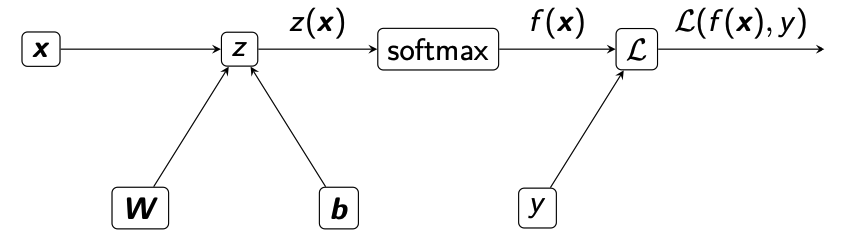
\includegraphics[width=.7\textwidth]{autodiff/computational-graph.png}
    \caption{Computational graph for $\L(\softmax(Wx+b), y)$}
    \label{fig:computational-graph}
\end{figure}
In Figure \ref{fig:computational-graph}, reading from left to right, we can see that the weights $W$, the biases $b$ and the input $x$ are combined to create a function $z(x)$; to the result of this operation is applied $\softmax$, creating $f(x)$. Finally, $f(x)$ is combined with $y$ using the loss function $\L$, giving the final result of the computation, $\L(f(x), y)$.

Computational graphs can then be used to apply the main algorithm to compute the gradient, called \emph{backpropagation}. We will illustrate its behavior by considering the function $f(x, y, z) = (x+y)\times z$, to which is associated the following computational graph:
\begin{figure}[H]
    \centering
    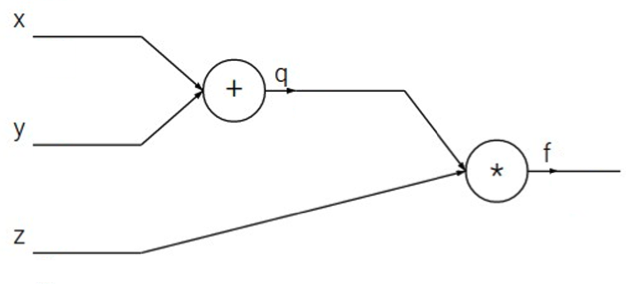
\includegraphics[width=.5\textwidth]{autodiff/simple-graph.png}
    \caption{Computational graph for $f(x, y, z) = (x+y)\times z$}
\end{figure}

\subsubsection{Forward pass}
The first step of backpropagation is to compute the outputs during a \emph{forward pass}. This is simply done by replacing each input by its numerical value, and applying the operations described by the nodes of the graph. Using $x=-2$, $y=5$, $z=-4$ in the previous example yields:
\begin{figure}[H]
    \centering
    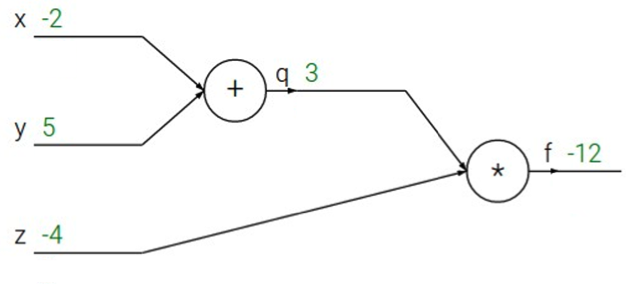
\includegraphics[width=.5\textwidth]{autodiff/forward-graph.png}
    \caption{Forward pass}
\end{figure}

\subsubsection{Backward pass}
The backward pass allows us to compute the derivatives, in our case $\partfrac{f}{x}$, $\partfrac{f}{y}$ and $\partfrac{f}{z}$. Instead of computing the value at each node from left to right (forward pass), we will compute the values of the derivatives from right to left, starting from the output (backward pass).

\begin{itemize}
    \item Starting from the output node, we have that $\partfrac{f}{f}=1$.
    \item Going backward to the $z$ input node, we have that $\partfrac{f}{z}=q$, since $f=qz$. We can then use the results of the forward pass to find the value of $q$, and deduce $\partfrac{f}{z}=3$.
    \item Similarly, $\partfrac{f}{q}=z=-4$.
    \item Going further back into the graph, we aim at computing $\partfrac{f}{y}$. Using chain rule, we know that:
    \begin{equation*}
        \partfrac{f}{y}=\partfrac{q}{y}\partfrac{f}{q}
    \end{equation*}
    This equation can be interpreted in terms of \say{gradient stream}: we want to compute the \emph{downstream gradient} $\partfrac{f}{y}$, that is the gradient \say{after the node}. This gradient can therefore be expressed using the chain rule as the product of the \emph{local gradient} $\partfrac{q}{y}$ and the \emph{upstream gradient} $\partfrac{f}{q}$, that is the gradient computed at the previous node.
    \begin{equation*}
        \underbrace{\partfrac{f}{y}}_{\textnormal{Downstream}}=\underbrace{\partfrac{q}{y}}_{\textnormal{Local}} \underbrace{\partfrac{f}{q}}_{\textnormal{Upstream}}
    \end{equation*}
    Like in previous cases, we can compute the local gradient $\partfrac{q}{y}=1$ since $q=x+y$. The upstream gradient is also known at this point of the pass, due to the backward direction, hence $\partfrac{f}{y}=1\times-4=-4$
    \item The same approach using the chain rule can be used for $\partfrac{f}{x}=\partfrac{q}{x}\partfrac{f}{q}=1\times -4=-4$.
\end{itemize}

\subsubsection{Modularity}
A benefit of backpropagation is its modularity: the gradient computation can be broke down into the computation of the downstream gradient knowing the upstream gradient and the local gradient of the node. 

Consider for instance a function $f$ taking $x$ and $y$ as inputs, and producing an output $z$. This function is a node somewhere in a possibly very complex computational graph, but we do not need the whole information about the rest of the computation: to compute the downstream gradient, we only need local information, that is upstream and local gradients. 

We are given the upstream gradient of the loss that we want to compute with respect to our output, $\partfrac{\L}{z}$. Our goal is now simply to propagate the gradient computation by providing the downstream derivatives, that is $\partfrac{\L}{x}$ and $\partfrac{\L}{y}$. Since we know the expression of $f$, we are able to compute the local derivatives $\partfrac{z}{x}$ and $\partfrac{z}{y}$; using chain rule, we can therefore provide the downstream gradient.
\begin{figure}[H]
    \centering
    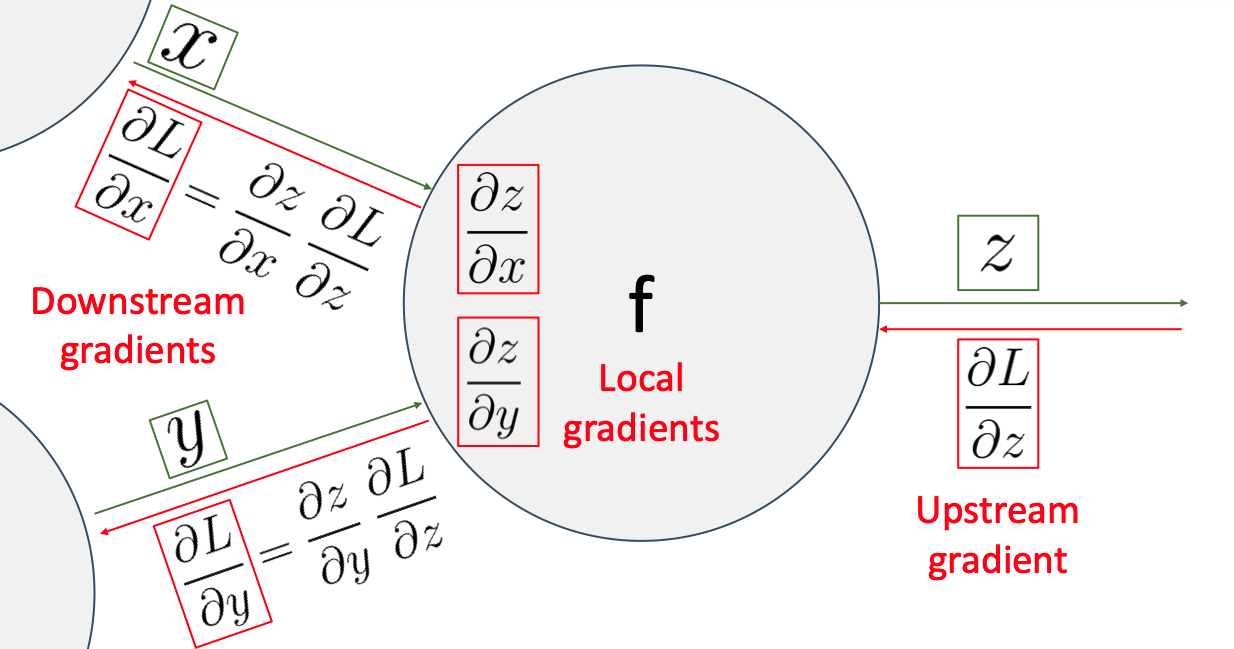
\includegraphics[width=.6\textwidth]{autodiff/modularity.png}
    \caption{Local process of computing the downstream gradient}
\end{figure}

\subsubsection{A complete example}
\begin{figure}[H]
    \centering
    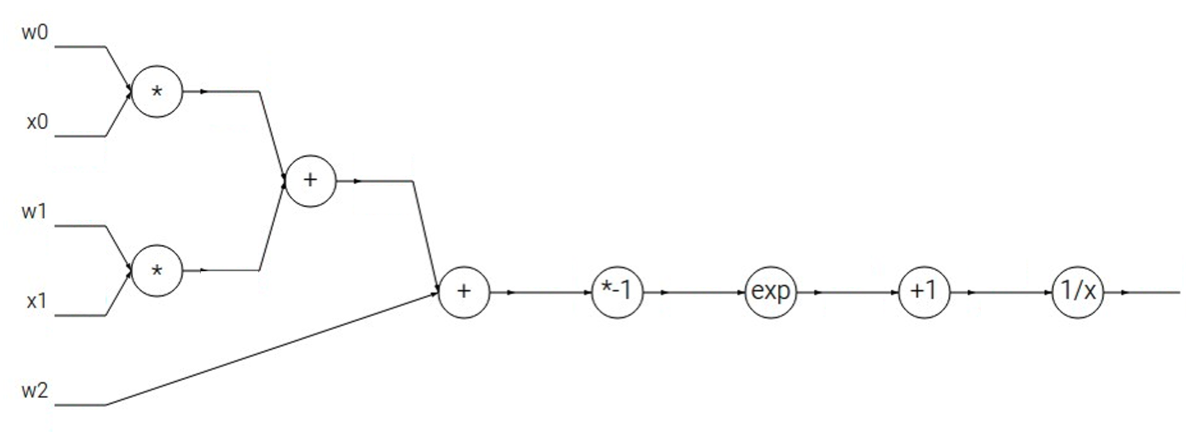
\includegraphics[width=.6\textwidth]{autodiff/complete-example.png}
    \caption{Computational graph for the function $f(x, w) = \frac{1}{1+e^{-(w_0x_0+w_1x_1+w_2)}}$}
\end{figure}
We do not have to break down the gradient computation only into elementary operations such as additions or multiplications: we can define blocks, such as \say{Sigmoid}, and hard-code their gradients to avoid using automatic differentiation on it.

\subsection{Extension to multivariate calculus}
So far, we only considered backpropagation in the case of scalars. The same principle can nevertheless be extended to multivariate calculus using vectors and matrices.

\subsubsection{Reminder on vector derivatives}
For a real-valued function $f:\R\longrightarrow\R$, the regular derivative is a scalar:
\begin{equation*}
    \frac{\dd f}{\dd x} = \partfrac{f}{x} \in \R
\end{equation*}

For a function taking a vector and returning a scalar, that is $f:\R^n\longrightarrow\R$, its derivative is its \emph{gradient}, that is:
\begin{equation*}
    \nabla f\in\R^n \where \left(\nabla f\right)_i = \partfrac{f}{x_i}
\end{equation*}
The $i$-coordinate of the gradient is the partial derivative of $f$ with respect to the $i$-th variable of the input vector.

Finally, for a differentiable function taking a vector and returning another vector, that is $f:\R^n\longrightarrow\R^m$, its derivative is its \emph{Jacobian}, that is:
\begin{equation*}
    J_f 
    = \begin{bmatrix} \partfrac{f}{x_1} & \dots & \partfrac{f}{x_n}\end{bmatrix} 
    = \begin{bmatrix} 
        \nabla^\tp f_1\\ 
        \vdots\\ 
        \nabla^\tp f_m
    \end{bmatrix}
    = \begin{bmatrix}
        \partfrac{f_1}{x_1} & \dots & \partfrac{f_1}{x_n}\\
        \vdots & \ddots & \vdots\\
        \partfrac{f_m}{x_1} & \dots & \partfrac{f_m}{x_n}
    \end{bmatrix}
    \in\mathscr{M}_{m, n}(\R)
\end{equation*}

\subsubsection{Example: linear layer gradient}
Consider a linear layer of the form $f(x)=Wx$ where $W$ is an $m\times n$ matrix. The $i$-th coordinate of the output of is
\begin{equation*}
    f_i = W_ix=\sum_j W_{i,j}x_j
\end{equation*}
where $W_i$ is the $i$-th row of $W$. Therefore, its Jacobian is:
\begin{equation*}
    (J_f)_{i, j} = \partfrac{f_i}{x_j} = W_{i, j}
\end{equation*}
hence $J_f=W$.

\subsubsection{Generalized multivariate chain rule}
Consider two differentiable functions $f:\R^m\longrightarrow\R^k$ and $g:\R^n\longrightarrow\R^m$, and $a\in\R^n$. The chain rule is expressed as:
\begin{equation}
    D_a(f\circ g) = D_{g(a)}f\circ D_ag
\end{equation}
where $D_af$ for instance is the derivative of $f$ evaluated in $a$. Furthermore, the Jacobians verify:
\begin{equation}
    J_{f\circ g}(a)=J_f(g(a)) J_g(a)
\end{equation}

% \section{Introduction to Reinforcement Learning}
\subsection{What is Reinforcement Learning?}
Machine learning problems can be distinguished in three major paradigms. Given a set of inputs and corresponding outputs, \emph{supervised learning} tries to learn the function mapping inputs to outputs. \emph{Unsupervised learning} studies the structure of data, without being given labels. The third paradigm is called \emph{reinforcement learning}: such problems aim at optimizing the actions of an agent in an environment to maximize its reward.

Formally, we control an agent that can observe at each time step $t$ the \emph{state} of the environment, $S_t$. It can use this state to choose an action $A_t$, to which the environment will reply with a reward $R_t$, and a new state $S_{t+1}$.
\begin{equation*}
    S_t\longrightarrow A_t\longrightarrow R_t \Longrightarrow S_{t+1}\longrightarrow A_{t+1} \longrightarrow \dots
\end{equation*}
This is called one \emph{episode} of learning.

\subsection{Markov Decision Process}
\subsubsection{Formalisation}
The \emph{Markov Decision Process} (MDP) is a mathematical formulation of the Reinforcement Learning process. It makes the assumption of the \emph{Markov property}: the current state completely caracterizes the state of the world.

\begin{definition}[Markov Decision Process]
    A Markov Decision Process is a 5-tuple $(\S, \A, \Rc, \P, \gamma)$ where:
    \begin{itemize}
        \item $\S$ is the set of all states
        \item $\A$ is the set of possible actions
        \item $\Rc:\S\times\A\to\R$ is a function mapping a (state, action) pair to an immediate reward
        \item $\P$ is a probability distribution; for $s,s'\in\S$, $a\in\A$, $\P(S_{t+1}=s'|S_t=s,A_t=a)$ is the probability to transition from state $s$ to state $s'$ after choosing the action $a$.
        \item $\gamma\in[0,1]$ is a \emph{discount factor}, quantifying how much we value rewards coming soon conversely to rewards coming later. $\gamma=1$ values equally all future rewards, while $\gamma=0$ means that we only care about the next reward.
    \end{itemize}

    Initially (at time step $t=0$), an initial state $S_0$ is sampled. Then for any $t\in\iset{0}{T}$\footnote{We might have $T=+\infty$} the following process is iterated:
    \begin{itemize}
        \item The agent chooses an action $A_t$
        \item The environment computes the associated reward $R_t=\Rc(S_t,A_t)$
        \item The environment samples the next step $S_{t+1}\sim\P(\cdot|S_t,A_t)$
        \item The agent receives the reward $R_t$ and the next step $S_{t+1}$
        \item \dots
    \end{itemize}
\end{definition}

\begin{definition}[Policy]
    A \emph{policy} $\pi:\S\to\A$ is a function that specifies which action to take in each state.
\end{definition}

We want to optimize the \emph{discounted return} (also known as \emph{cumulative discounted reward}), that is:
\begin{equation*}
    G_t=R_{t+1}+\gamma R_{t+2}+\dots+\gamma^{T-t-1}R_T = \sum_{k=t+1}^T\gamma^{k-t-a}R_k
\end{equation*}
Note that the discounted return $G_t$ is a random variable, since the rewards $(R_k)_k$ depend on the sampled states $(S_k)_k$. 
Therefore, we introduce the following two deterministic functions.
% Therefore, we introduce the following deterministic function.

\begin{definition}[Value function]
    Given a policy $\pi$, the \emph{value function} $v_\pi$ is defined by:
    \begin{equation*}
        v_\pi(s) = \E\left[G_t|S_t=s\right]
    \end{equation*}
    where the expectation is taken over the sampled states $(s_k)_{k>t}$ and in which the successive actions $A_k$ are picked using the policy: $A_k=\pi(S_k)$.
\end{definition}

\begin{definition}[Action-value function]
    Given a policy $\pi$, the \emph{action-value function} $q_\pi$ is defined by:
    \begin{equation*}
        q_\pi(s, a) = \E\left[G_t|S_t=s, A_t=a\right]
    \end{equation*}
    where the expectation is taken over the sampled states $(s_k)_{k>t}$. The difference with the value function is that we assume that the action $a$ is taken, making it in a sense \say{one episode after}.
\end{definition}
Note that:
\begin{equation*}
    v_\pi(s)=q_\pi(s,\pi(s))
\end{equation*}

These functions can be used in two ways. The first is policy evaluation: given a policy $\pi$, compute its value function, acting as a metric to measure how good a policy is. 
% Note that:
% \begin{equation*}
%     v_\pi(s)=\E_a[q_\pi(s,a)] = \sum_{a\in\A}\pi(a|s)\cdot q_\pi(s,a)
% \end{equation*}
Another goal can be \emph{policy improvement}: given $v_\pi$, improve $\pi$ by picking the best possible action $a^*$:
\begin{equation*}
    a^* = \argmax_a q_\pi(s,a)
\end{equation*}
Note that we therefore have:
\begin{equation*}
    q_\pi(s,a^*) = \E_{s'}\left[r+\gamma v_\pi(s')\right] = \sum_{s'}\P(s'|s,a)\cdot[r+\gamma\cdot v_\pi(s')]
\end{equation*}

\subsubsection{Example: Gridworld}
Let's analyze a simple example of Reinforcement Learning problem. Gridworld is a task in which the states are the positions in the grid, and the actions are the movements in all 4 directions. The goal is two reach one of the terminal states, in the least number of actions.

Formally, we can define a Markov decision process by setting:
\begin{equation*}
    \S=\set{(i,j)}{1\leq i,j\leq5} \qquad \A=\{\leftarrow,\rightarrow,\uparrow,\downarrow\} \qquad \Rc=s\longmapsto-1
\end{equation*}

% TODO: TikZ figure for the grid and optimal policy

\subsubsection{Optimal policy}
The optimization problem associated with the Markov Decision Process is to select the best policy, that is the policy which maximizes the expected discounted return:
\begin{equation}
    \pi^*=\argmax_\pi \E[G_t]
\end{equation}
where the expectation is taken over the sampled states $(S_k)_{k>t}$ and in which the successive actions $A_k$ are picked using the policy: $A_k=\pi(S_k)$.

\begin{definition}[Optimal action-value function]
    The optimal action-value function $q^*$ is the maximum expected cumulative reward achievable from a given (state, action) pair:
    \begin{equation*}
        q^*(s,a) = \max_\pi\E\left[G_t|S_t=s,A_t=a\right]
    \end{equation*}
\end{definition}

\begin{theorem}[Bellman's principle of optimality -- 1952]
    An optimal policy has the property that whatever the initial state and initial decision are, the remaining decisions must constitute an optimal policy with regard to the state resulting from the first decision.
\end{theorem}

\begin{property}[Bellman's equation]
    Intuitively, if the optimal state-action values for the next time-step $q^*(s',a)$ are known, then the optimal strategy is to take the action that maximizes the expected value of $r+ \gamma\cdot q^*(s, a)$. Formally, this gives us:
    \begin{equation}
        q^*(s,a) = \E_{s'}\left[r+\gamma\cdot\max_{a'}q^*(s',a')|s,a\right]
    \end{equation}
    Therefore, the optimal policy takes in each state the action maximizing $q^*(s,a)$.
\end{property}

\subsubsection{Value iteration algorithm}
We can derive an iterative update from Bellman's equation:
\begin{equation*}
    q_{i+1}(s,a) = \E\left[r+\gamma\cdot\max_{a'}q_i(s',a')|s,a\right]
\end{equation*}
At each step, we refine our approximation of $q^*$ by following Bellman's equation. Under mathematical conditions, we will then have:
\begin{equation*}
    \lim_{i\to+\infty}q_i = q^*
\end{equation*}

Unfortunately, this idea is not scalable: it requires the computation of $q(s,a)$ for every (state, action) pair, even though the state space can be huge. For instance, if we try to apply this reinforcement learning approach to a video game, we need to compute the result for any combination of pixels on the screen.

Therefore, we use in practice an approximator of $q$ instead of computing the exact value of $q$: this is called Q-learning. 
\newpage
\section{Optimization and loss functions}
\subsection{Tensors in \texttt{PyTorch}}
A tensor is a $d$-dimensional array in \texttt{PyTorch}. Tensors are used in deep learning to represent all kind of data, from images to weight matrices.

\paragraph*{Tensor creation}
A tensor can be created from a list: \mintinline{python}{x = torch.Tensor([[1,0,2],[3,2,2]])}. By default, tensors are not deepcopied, but can be cloned: \mintinline{python}{x.clone()}. Each tensor has a data type, which can be specified at its creation: \mintinline{python}{x = torch.Tensor(..., dtype=torch.int64)}. In the case of data (for instance, training examples), the first dimension of a tensor is usually the samples: \mintinline{python}{x.shape[0]} is the batch size.

\paragraph*{Operations}
Most operations on tensors (\mintinline{python}{+}, \mintinline{python}{*}, \dots) are performed coordinate-wise and need matching sizes. Mathematical functions from the \mintinline{python}{torch} library, such as \mintinline{python}{torch.exp} or \mintinline{python}{x**2}, are vectorized and therefore performed coordinate-wise. Notably, matrix multiplication can be perfomed using the \mintinline{python}{x @ y} syntax.

\paragraph*{Shapes}
A tensor shape can be obtained by calling \mintinline{python}{x.shape}. Reshaping can be performed using \mintinline{python}{x.view(1,3,-1)}, where \mintinline{python}{-1} acts as a wildcard for \texttt{PyTorch} to fill in automatically the appropriate dimension. For instance, \mintinline{python}{x.view(-1)} flattens the tensor into a one-dimensional vector. The operation \mintinline{python}{x.unsqueeze(0)} adds a dimension of size 1 to the tensor.

\paragraph*{Gradients}
Tensors can have an associated gradient, stored in \mintinline{python}{x.grad}. We can remove (and clone) this tensor from the computation of the gradient by using \mintinline{python}{y = x.detach()}.

\paragraph*{Other operations}
See the \href{https://pytorch.org/docs/stable/tensors.html}{\texttt{PyTorch} documentation} for numerous operations defined on tensors. Most convenient ones include \mintinline{python}{torch.sum(x)}, \mintinline{python}{torch.mean(x)}. A tensor can also be converted to a \texttt{NumPy} array using \mintinline{python}{x.numpy()} or \mintinline{python}{x.detach().numpy()}.

Manipulating tensors and tensor sizes is complex and leads to many bugs in deep learning projects. Many errors can go unnoticed due to wrong tensor sizes and Python's dynamic typing. As a general advice, always verify your intermediate computations using for instance \mintinline{python}{print(x[:5])}, and your tensor shapes with \mintinline{python}{print(x.shape)}!

\subsection{Loss functions}
\subsubsection{Mean Square Error}
\begin{definition}[Mean Square Error]
    The \emph{mean square error} is the loss function defined by:
    \begin{equation*}
        \begin{aligned}
            \ell : \R^d\times\R^d&\longrightarrow\R\\
            x, y&\longmapsto \norm{x-y}_2^2 = (x-y)^\tp(x-y)
        \end{aligned}
    \end{equation*}
\end{definition}

MSE has a probabilistic interpretation, fitting the following probabilistic model: we are trying to learn a certain function $g_\theta$, parametered by $\theta\in\R^p$. To do so, we are given tuples of data of the form $(X_i, Y_i)$, where $Y_i$ is the label corresponding to $X_i$. We assume that the probabilistic relationship between $X_i$ and $Y_i$ is the following:
\begin{equation*}
    Y_i=g_\theta(X_i)+\epsilon_i
\end{equation*}
where $\epsilon_i\sim\mathcal{N}(0,\sigma^2I_d)$ are i.i.d.~centered Gaussian random variables (that is of mean 0 and variance $\sigma^2$). We also assume that the $X_i$ are i.i.d.~and independent of $\theta$.

Let's apply the Maximum Likelihood principle to this probabilistic model. The likelihood for the data to be drawn from a given $\theta$ is:
\begin{equation*}
    \begin{aligned}
        \P_\theta((X_i,Y_i)_i)&=\prod_i \P(X_i) \cdot \P_\theta\left(\epsilon_i=Y_i-g_\theta(X_i)\right)\\
        &=\prod_i \P(X_i) \cdot \frac{1}{\sqrt{(2\pi)^d|\sigma^2I_d|}}\cdot\exp\left(-\frac{1}{2}(Y_i-g_\theta(X_i)-0)^\tp(\sigma^2I_d)^{-1}(Y_i-g_\theta(X_i)-0)\right) \\
        &=\prod_i \frac{\P(X_i)}{\sqrt{(2\pi\sigma^2)^d}}\cdot\exp\left(-\frac{1}{2\sigma^2}\norm{Y_i-g_\theta(X_i)}_2^2\right) \\
        &\propto\exp\left(-\frac{\sum_i\norm{Y_i-g_\theta(X_i)}_2^2}{2\sigma^2}\right)\\
        &= \exp\left(-\frac{\ell(Y_i,g_\theta(X_i))}{2\sigma^2}\right)
    \end{aligned}
\end{equation*}
Therefore, maximizing the $\log$-likelihood is equivalent to minimizing the MSE.

In \texttt{PyTorch}, means square error can be used with the line \mintinline{python}{criterion = nn.MSELoss()}. It supports several parameters, such as \mintinline{python}{reduction='sum'}, \mintinline{python}{reduction='mean'}, which are described in \href{https://pytorch.org/docs/stable/generated/torch.nn.MSELoss.html}{the documentation}. Once set, \mintinline{python}{criterion} takes as input two tensors of shapes $[N,d]$, where $N$ is the batch size and $d$ is the dimension of the output vectors. Note that when $d=1$, the output should be of size $[N,1]$ and not $[N]$; in that case, \mintinline{python}{x.unsqueeze(-1)} can come in handy.

\subsubsection{Cross Entropy}
\begin{definition}[Cross Entropy]
    The \emph{cross entropy} is the loss function defined by:
    \begin{equation*}
        \begin{aligned}
            \ell : \R^C\times\iset{1}{C}&\longrightarrow\R\\
            x, y&\longmapsto -\log\left(\frac{\exp(x_y)}{\sum_i\exp(x_i)}\right)
        \end{aligned}
    \end{equation*}
\end{definition}

Similarly to MSE, minimizing the cross entropy corresponds to maximizing the $\log$-likelihood for a certain probabilistic model. Assume that there is a parameter $\theta\in\R^p$ such that, for all classes $k\in\iset{1}{C}$,
\begin{equation*}
    \log\P(Y_i=k|X_i) \propto g_\theta(X_i)_k
\end{equation*}
where $X_i$ are i.i.d.~and independent of $\theta$. Then, the likelihood for the data to be drawn for a given $\theta$ is:
\begin{equation*}
    \begin{aligned}
        \P_\theta((X_i,Y_i)_i) &= \prod_i\P(X_i)\cdot\P_\theta(Y_i|X_i)\\
        &\propto\prod_i\frac{\exp(g_\theta(X_i)_{Y_i})}{\sum_k\exp(g_\theta(X_i)_k)}
    \end{aligned}
\end{equation*}

In \texttt{PyTorch}, cross entropy can be used with the line \mintinline{python}{criterion = nn.CrossEntropyLoss()}. It supports several parameters, such as \mintinline{python}{reduction='sum'}, \mintinline{python}{reduction='mean'}, which are described in \href{https://pytorch.org/docs/stable/generated/torch.nn.MSELoss.html}{the documentation}. Once set, \mintinline{python}{criterion} takes as input two tensors: the \emph{scores} (a tensor of shape $[N,C]$), and either a class index per sample, or class probabilities for each sample. Note that \mintinline{python}{nn.CrossEntropyLoss} is the composition of \mintinline{python}{nn.LogSoftmax} and \mintinline{python}{nn.NLLLoss}.

Finally, be aware that gradient can explode when going through a softmax, due to numerical errors. This is however taken care of by the \texttt{PyTorch} implementation of \mintinline{python}{nn.CrossEntropyLoss} and \mintinline{python}{nn.LogSoftmax}.

\subsection{First-order optimization}
\subsubsection{Introduction}
Given an objective function $\L:\R^d\longrightarrow\R$, the goal of optimization is to find a minimized $\theta^*\in\R^d$ of $\L$, that is:
\begin{equation*}
    \theta^*\in\argmin_{\theta\in\R^d}\L(\theta)
\end{equation*}
A standard approach to doing so is to use an iterative algorithm relying on the gradient $\nabla\L(\theta_t)$ at each iteration $t\geq0$.
\begin{figure}[H]
    \centering
    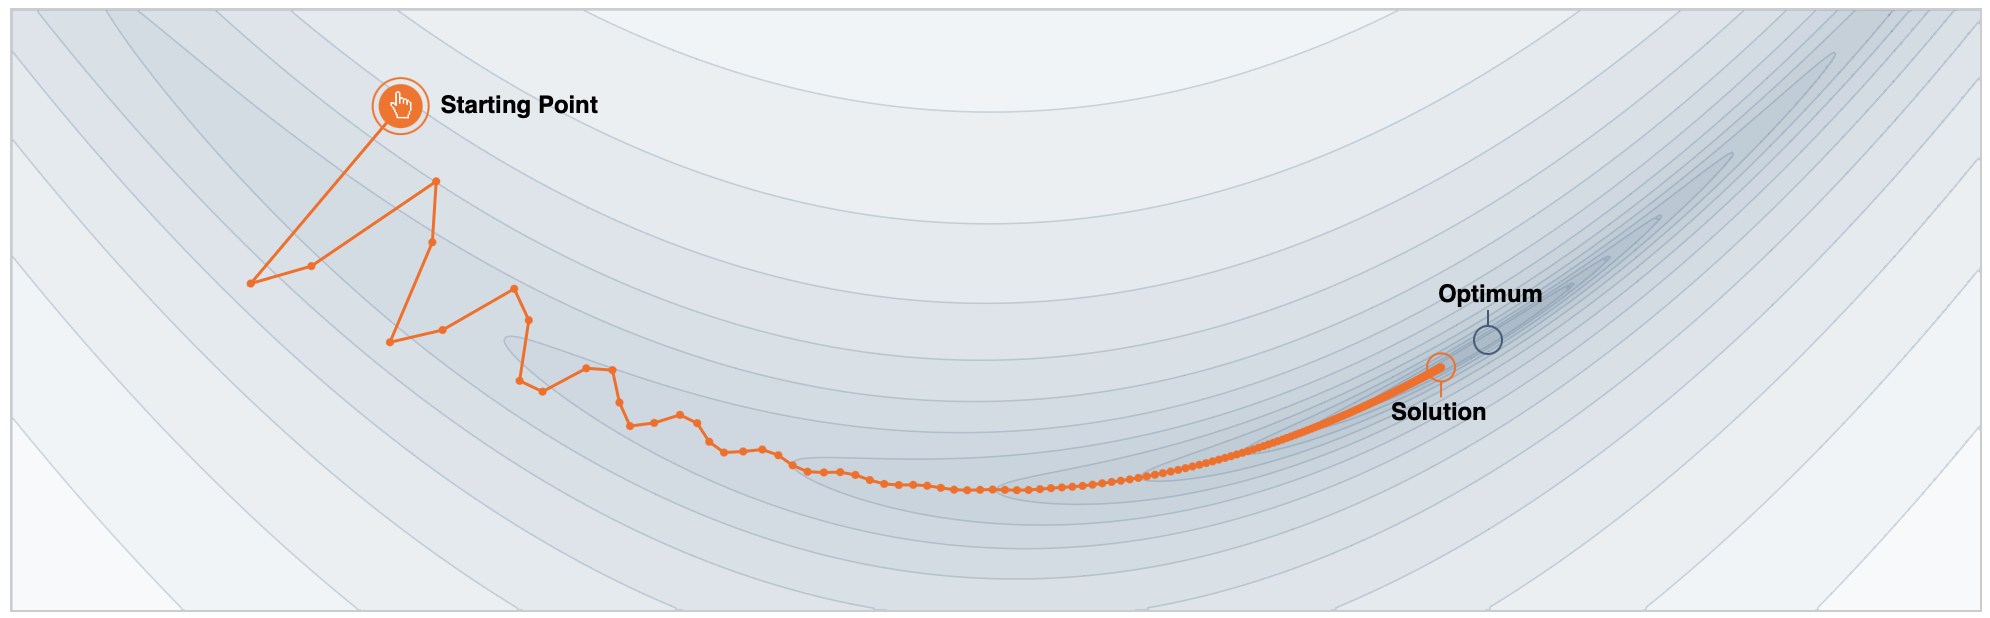
\includegraphics[width=.9\textwidth]{optimization-loss/distill-momentum.png}
    \caption{Simulation of gradient descent from \href{https://distill.pub/2017/momentum/}{\nolinkurl{https://distill.pub/2017/momentum/}}.}
\end{figure}

\subsubsection{Gradient descent structure}
Iterative optimization algorithms all follow the same structure:
\begin{description}
    \item[Initialization] We start with a random parameter $\theta_0\in\R^p$. The choice of the initial value is very important in practice, as a good initialization will help our model to converge and reduce overfitting.
    \item[Iteration] The current value of the parameter is updated using a rule of the form
    \begin{equation*}
        \theta_{t+1}=\phi_t(\theta_t,\nabla\L(\theta_t),s_t)
    \end{equation*}
    where $s_t$ is a hidden variable that is also updated at each iteration. The update function, $\phi_t$, might depend on the step $t$ (for instance when using various step sizes). The most basic version of gradient descent is $\theta_{t+1}=\theta_t-\eta\cdot\nabla\L(\theta_t)$, where $\eta$ is the learning rate (or step size).
    \item[Stopping time] The algorithm stops after a certain number $T$ of iterations. This is important in practice and $T$ should be picked carefully to avoid overfitting.
\end{description}

\subsubsection{Difficulties in neural network training}
In practice, training deep neural network can become challenging because of numerous difficulties.
\begin{description}
    \item[Non-convexity] If $\L$ is convex, that is:
    \begin{equation*}
        \forall\theta,\theta'\in\R^p, \quad \L\left(\frac{\theta+\theta'}{2}\right) \leq \frac{\L(\theta)+\L(\theta')}{2}
    \end{equation*}
    the optimization problem is fairly simple. Most theoretical results use this assumption in order to prove the convergence of the algorithm. In practice, this is often not the case, making the optimization problem very hard.
    \item[High dimensionality] The number of parameters $d$ can be huge: for instance, the VGG-16 network, a convolutional neural network trained on the ImageNet dataset, has $p=138\,357\,544$ parameters.
    \item[Access to the gradient] The gradient of $\L$ is often too expensive to compute on the entire dataset. In practice, $\nabla\L(\theta_t)$ is replaced by a stochastic or mini-batch approximation $\tilde{\nabla}_t$.
\end{description}

\subsubsection{Gradient approximations}
In the following, we will consider that the objective function $\L$ is a loss function between a prediction and a label for one specific example, that is:
\begin{equation*}
    \forall i\in\iset{1}{n}, \quad \L_i(\theta) = \ell(g_\theta(x_i),y_i)
\end{equation*}
Our objective function $\L$ will be the training error:
\begin{equation*}
    \L(\theta) = \frac{1}{n}\sum_{i=1}^n \L_i(\theta) =  \frac{1}{n}\sum_{i=1}^n \ell(g_\theta(x_i),y_i)
\end{equation*}
In the following, $\eta>0$ denotes a \emph{learning rate} (or \emph{step-size}). The following variants of gradient descent are often used:
\begin{description}
    \item[Batch gradient descent] It uses the true gradient:
    \begin{equation*}
        \theta_{t+1} = \theta_t-\eta\cdot\frac{1}{n}\sum_{i=1}^n\nabla\L_i(\theta)
    \end{equation*}
    This approach gives the best possible gradient, but is very expensive if the dataset is large (when $n$ is big).
    \item[Stochastic gradient descent] The gradient is approximated with one random sample
    \begin{equation*}
        \theta_{t+1} = \theta_t-\eta\cdot\L_{i_t}(\theta)
    \end{equation*}
    This approach is very efficient but often instable, since one element might contain noise, making the convergence difficult.
    \item[Mini-batch gradient descent] The gradient is approximated with multiple random samples:
    \begin{equation*}
        \theta_{t+1} = \theta_t-\eta\cdot\frac{1}{b}\sum_{i=1}^b\nabla\L_{i_{b,t}}(\theta)
    \end{equation*}
    where $b>0$ is the \emph{batch size}. This method is a good tradeoff between speed and convergence, with a parameter $b$ that can be adjusted to obtain the best results.
\end{description}

Keep in mind that the final goal is to reduce the population risk, that is $\E[\ell(g_\theta(X), Y)]$. We need to pay attention to overfitting in addition to using the optimization algorithm to reduce the training error. In this class, we focus specifically on the performance of the optimization algorithm in minimizing the objective function, rather than the model's generalization error. In the next chapters, we will see techniques to avoid overfitting.

\subsection{Convergence analysis}
We aim at providing theoreticla guarantees over the convergence rates of our algorithms. Optimizing non-convex functions is hard in general, but we will make the following assumptions:
\begin{itemize}
    \item The objective function is non-convex but differentiable and $\beta$-smooth, that is:
    \begin{equation*}
        \forall\theta,\theta'\in\R^p, \quad \norm{\nabla\L(\theta)-\nabla\L(\theta')}_2 \leq \beta\cdot\norm{\theta-\theta'}_2
    \end{equation*}
    \item We access unbiased noisy gradients $\tilde{\nabla}_t$, where:
    \begin{equation*}
        \E[\tilde{\nabla}_t] = \nabla\L(\theta_t) \quad \textnormal{and} \quad \V[\tilde{\nabla}_t] \leq\sigma^2
    \end{equation*}
\end{itemize}

\begin{property}[Worst-case convergence to global optimum]
    For any first-order algorithm, there exists a smooth function $\L$ such that its approximation error is at least:
    \begin{equation*}
        \L(\theta_t)-\L(\theta^*) = \Omega(t^{-\frac{1}{d}})
    \end{equation*}
\end{property}
This is prohibitive for large dimensional spaces, since this makes the convergence extremly slow. Therefore, we often choose to restrict ourselves to guarantees for local optima.

\begin{theorem}[Convergence of non-convex SGD to a stationary point]
    Let $\L:\R^p\to\R$ be a smooth function and $\Delta=\L(\theta_0)-\L(\theta^*)$. Then, SGD with step-size:
    \begin{equation*}
        \eta=\min\left(\frac{1}{\beta}, \sqrt{\frac{2\Delta}{T\beta\sigma^2}}\right)
    \end{equation*}
    achieves the error:
    \begin{equation*}
        \E\left[\min_{t\leq T}\norm{\nabla\L(\theta_t)}^2\right] \leq \frac{4\beta\Delta}{T} + \sqrt{\frac{8\beta\Delta\sigma^2}{T}}
    \end{equation*}
    Furthermore,
    \begin{itemize}
        \item without noise, $\eta=\frac{1}{\beta}$ is optimal, and require $O\left(\frac{\beta\Delta}{\epsilon^2}\right)$ iterations for $\norm{\nabla\L(\theta_t)}\leq\epsilon$
        \item with noise, $\eta=O\left(T^{-\frac{1}{2}}\right)$ is optimal, and requires $O\left(\frac{\beta\Delta\sigma^2}{\epsilon^4}\right)$ iterations for $\norm{\nabla\L(\theta_t)}\leq\epsilon$
        \item if $\eta$ is fixed and $\sigma>0$, there is a lower limit in $O\left(\sqrt{\eta\beta}\sigma\right)$ for $\norm{\nabla\L(\theta_t)}$
    \end{itemize}
\end{theorem}

These guarantees prove that GD and SGD converge to a stationary point. Nevertheless, we have no guarantee that this stationary point is actually a local minimum. A local minimum can be defined using second order derivatives: it is both a \textbf{stationary} point, that is $\nabla\L(\theta)=0$, and a \textbf{convexity} point, where the Hessian $H_\L(x)$ is semi-definite positive. The problem is that stationary points can block our algorithm by cancelling the gradient: we are then stuck in saddle points.

An idea to converge towards a local minimum is to add a small noise, allowing the parameter to escape saddle points. When slightly pushed away from the equilibrium by the noise, the parameter will come back to it only is the equilibrium is stable, that is for local minima.

We make the additional assumption that the Hessian $H_\L$ is $\rho$-Lipschitz with respect to the spectral norm. Therefore, with probability at least $1-\delta$, the number of iterations to reach a gradient norm $\norm{\nabla\L(\theta_t)}\leq\epsilon$ and near-convexity $\lambda_1(H_\L(\theta_t))\geq-\sqrt{\rho\epsilon}$ is bounded by:
\begin{equation*}
    O\left(\frac{\beta\Delta}{\epsilon^2}\cdot\log\left(\frac{p\beta\Delta}{\epsilon\delta}\right)^4\right)
\end{equation*}

To conclude:
\begin{itemize}
    \item The loss landscape of deep learning training is non-convex and potentially difficult to optimize
    \item SGD converges to a stationary point in $O(\epsilon^{-4})$ iterations
    \item GD converges to a stationary point in $O(\epsilon^{-2})$ iterations
    \item Adding small noise to GD make it converge to a local minimum in $O(\epsilon^{-2}\log(\epsilon^{-1})^4)$ iterations.
    \item Convergence to a global minimum is prohibitive in high-dimensional spaces. We need at least $\Omega(\epsilon^{-d})$ iterations for smooth functions; we need additional assumptions to ensure fast rates, such as the Polyak-Losasiewicz condition.
\end{itemize}

\subsection{Gradient descent variants}
Mini-batch gradient descent is the algorithm of choice when training a neural network. The term SGD is usually employed even when mini-batches are used! But despite working very well on fundamental examples (such as MLPs), some important questions remain. For instance, choosing learning rates can be difficult: how can we adapt the learning rate during training? Do we apply the same learning rate to all parameter updates? How to espace saddle points when the gradient is close to zero in all dimensions? We will introduce modifications to SGD to address these issues.\footnote{For more information, you can read \href{https://www.ruder.io/optimizing-gradient-descent/}{this nice survey} by Sebastian Ruder of different gradient descent optimization algorithms.}

\subsubsection{Momentum}
The core idea of \emph{momentum} is to accelerate SGD by dampening oscillations, that is averaging the last values of the latest gradients. We maintain a hidden state $v_t$ which is updated at each step, and used to update the parameter:
\begin{equation*}
    \begin{aligned}
        v_{t+1} &= \gamma\cdot v_t+\eta\cdot\nabla\L(\theta_t)\\
        \theta_{t+1} &= \theta_t - v_{t+1}
    \end{aligned}
\end{equation*}
where $\gamma$ is a decay factor, with a typical value of $\gamma=0.9$. Intuitively, $v_t$ will store a sort of average of the previous gradients; note that:
\begin{equation*}
    \forall k\geq 0, \quad v_{t+1} = \gamma^k\cdot v_{t-k} + \eta\sum_{i=0}^k \gamma^i \nabla\L(\theta_{t-i})
\end{equation*}
If we choose $v_0=0$, then we have:
\begin{equation*}
    \quad v_{t+1} = \eta\sum_{i=0}^t \gamma^{t-i} \nabla\L(\theta_i)
\end{equation*}
which corresponds to a weighted sum of the previous gradients, each with a factor decreasing as the number of iterations increases.

\subsubsection{Nesterov accelerated gradient}
With momentum, we first compute the gradient and then make a step following our momentum and add the gradient. Nesterov proposed to first make the step following the momentum, and then adjusting by computing the gradient locally. Formally, this gives us:
\begin{equation*}
    \begin{aligned}
        v_{t+1} &= \gamma\cdot v_t + \eta\cdot\nabla\L(\theta_t-\gamma\cdot v_t)\\
        \theta_{t+1} &= \theta_t - v_{t+1}
    \end{aligned}
\end{equation*}
\begin{figure}[H]
    \centering
    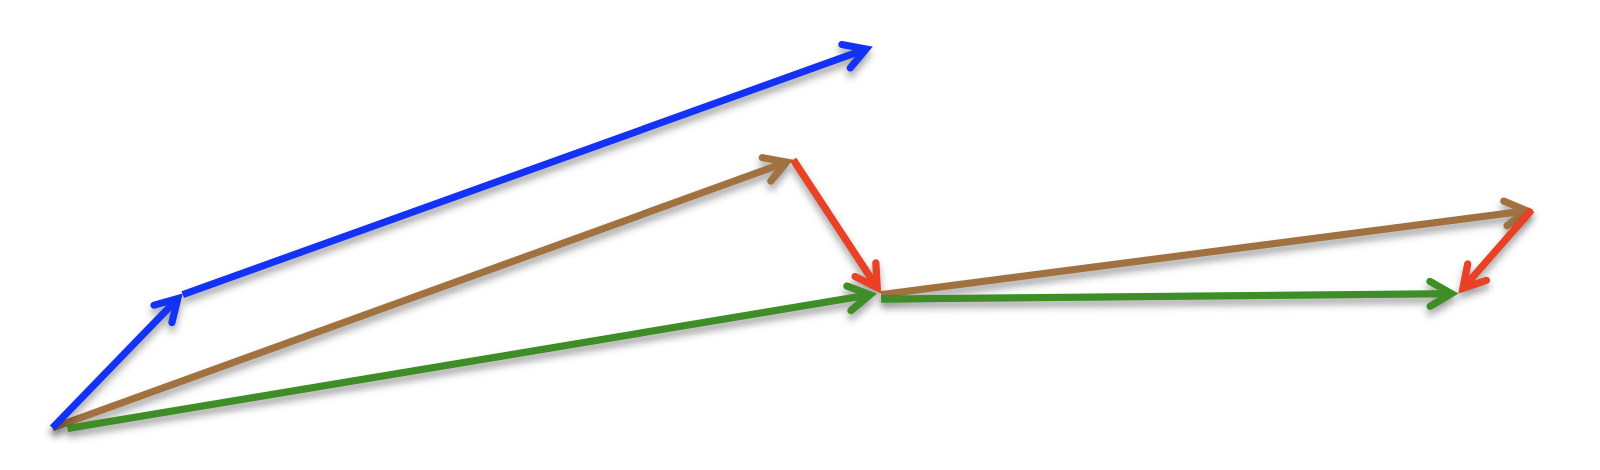
\includegraphics[width=.7\textwidth]{optimization-loss/nesterov.png}
    \caption{Nesterov method. Brown corresponds to the accumulated gradient jump $\gamma\cdot v_t$, red to the gradient correction $\eta\cdot\nabla\L(\theta_t-\gamma\cdot v_t)$, and blue to the standard momentum.}
\end{figure}

\subsubsection{AdaGrad}
We would like to adapt our updates to each individual parameter, i.e.~have a different decreasing learning rate for each parameter. This is what AdaGrad (standing for Adaptative Gradient) does:
\begin{equation*}
    \begin{aligned}
        s_{t+1,i} &= s_{t,i} + \nabla\L(\theta_t)_i^2\\
        \theta_{t+1,i} &= \theta_{t,i} - \frac{\eta}{\sqrt{s_{t+1,i}+\epsilon}}\cdot\nabla\L(\theta_t)_i
    \end{aligned}
\end{equation*}
This provides a decreasing learning rate, allowing to go fast at the beginning and slower when approaching the minimum. This requires no manual tuning of the learning rate. Typical default values are $\eta=0.01$ and $\epsilon=10^{-8}$.

\subsubsection{RMSProp}
The problem with AdaGrad is that the learning rate goes to zero, and never forgets about the past. An idea to avoid this is to use an exponential average instead:
\begin{equation*}
    \begin{aligned}
        s_{t+1,i} &= \gamma\cdot s_{t,i} + (1-\gamma)\cdot\nabla\L(\theta_t)_i^2\\
        \theta_{t+1,i} &= \theta_{t,i} - \frac{\eta}{\sqrt{s_{t+1,i}+\epsilon}}\cdot\nabla\L(\theta_t)_i
    \end{aligned}
\end{equation*}
where $\gamma$ is a decay factor (similarly to the idea of momentum), with default values $\gamma=0.9$ and $\eta=0.001$.

\subsubsection{Adam}
From the algorithm variations presented previously emerge two big ideas: using momentum to store the gradient, and having individual learning rates. Combining RMSProp and momentum gives us a widely used algorithm, Adam (for Adaptative Moment Estimation). It uses the following equations:
\begin{equation*}
    \begin{aligned}
        m_{t+1} &= \beta_1\cdot m_t + (1-\beta_1)\cdot\nabla\L(\theta_t)\\
        v_{t+1} &= \beta_2\cdot v_t + (1-\beta_2)\cdot\nabla\L(\theta_t)^2\\
        \hat{m}_{t+1} &= \frac{m_{t+1}}{1-\beta_1^{t+1}}\\
        \hat{v}_{t+1} &= \frac{v_{t+1}}{1-\beta_2^{t+1}}\\
        \theta_{t+1} &= \theta_t - \frac{\eta}{\sqrt{\hat{v}_{t+1}}+\epsilon}\cdot\hat{m}_{t+1}
    \end{aligned}
\end{equation*}
While they seem complex, these are just the extension and combinaison of the algorithms detailled before. $m_t$ and $v_t$ are estimates for the first and second moments of the gradients, just like we used in momentum and RMSProp. Because $m_0=v_0=0$, these estimates are biased towards $0$, thus the factors $(1-\beta^{t+1})^{-1}$ are here to counteract these biases. Typical values are $\beta_1=0.9$, $\beta_2=0.999$ and $\epsilon=10^{-8}$.

\subsubsection{AMSGrad}
Sometimes, Adam forgets too fast. To fix it, we replace the moving average by a $\max$ operator:
\begin{equation*}
    \begin{aligned}
        m_{t+1} &= \beta_1\cdot m_t + (1-\beta_1)\cdot\nabla\L(\theta_t)\\
        v_{t+1} &= \beta_2\cdot v_t + (1-\beta_2)\cdot\nabla\L(\theta_t)^2\\
        \hat{v}_{t+1} &= \max(\hat{v}_t, v_{t+1})\\
        \theta_{t+1} &= \theta_t - \frac{\eta}{\sqrt{\hat{v}_{t+1}}+\epsilon}\cdot m_{t+1}
    \end{aligned}
\end{equation*}

\subsection{\texttt{PyTorch} optimizers}
All these optimizers are built-in in \texttt{PyTorch}. They share the similar constructor:
\begin{center}
    \mintinline{python}{torch.optim.*(params, lr=..., momentum=...)}
\end{center}
Default values are different for all optimizers. In this construction, \mintinline{python}{params} should be an iterable (like a list) containing the parameters to optimize over. It can be obtained from any model with \mintinline{python}{module.parameters()}. The \mintinline{python}{setp} method updates the internal state of the optimizer acoording to the \mintinline{python}{grad} attributes of the \mintinline{python}{params}, and updates the latter according to the internal state.

A simple training loop is of the form:
\begin{figure}[H]
    \centering
    \begin{minipage}[t]{.7\textwidth}
        \begin{minted}{python}
criterion = nn.NLLLoss()
optimizer = torch.optim.SGD(model.parameters(),lr = 0.001)
model.train()
for epoch in range(num_epochs):
    for inputs, targets in dataloader:
        inputs, targets = inputs.to(device), targets.to(device)
        optimizer.zero_grad()
        outputs = model(inputs)
        loss = criterion(outputs, targets)
        loss.backward()
        optimizer.step()
        \end{minted}
        \caption{A simple \texttt{PyTorch} training loop.}
    \end{minipage}
\end{figure}
\section{Convolutional Neural Networks}
\subsection{Introduction}
\emph{Convolutional Neural Networks} (CNNs) is a class of models widely used in computer vision. While Fully Connected Neural Networks are very powerful machine learning models, they do not respect the 2D spatial structure of the input images. For instance, training a Multilayer Perceptron on a dataset of $32\times 32$ images required the model to start with a \texttt{Flatten} layer, that reshaped matrix images of size \texttt{(32, 32)} to flattened vectors of size \texttt{(1024, 1)}. Similarly, different color channels were handled separately, reshaping tensor images of dimensions \texttt{(32, 32, 3)} to \texttt{(3072, 1)}.

\begin{figure}[H]
    \centering
    \begin{tikzpicture}
        \newcommand{\randint}{
            \pgfmathsetmacro{\temp}{random(0, 1)}
            \temp
        }
        \fill[orange!60] (-1.9, -1.9) rectangle (1.9, 1.9);
        \matrix [
            matrix of math nodes,
            nodes={
                minimum size=1em, 
                outer sep=0pt,
                inner sep=0,line
                width=0.5pt,
                append after command={
                    \pgfextra{\draw[thick] 
                    ($(\tikzlastnode.north west)+(-0.4em,+0.4em)$)
                    rectangle ($(\tikzlastnode.south east)+(0.4em,-0.4em)$);}
                }
            },
            nodes in empty cells,
            column sep=-0.5pt,
            row sep=-0.5pt
        ]
        {
            \randint & \randint & \randint & \randint & \randint \\
            \randint & \randint & \randint & \randint & \randint \\
            \randint & \randint & \randint & \randint & \randint \\
            \randint & \randint & \randint & \randint & \randint \\
            \randint & \randint & \randint & \randint & \randint \\
        };

        \draw[<->, thick] (-1.9, -2.1) -- (1.9, -2.1) node[below, pos=0.5] {$32$};
        \draw[<->, thick] (-2.1, -1.9) -- (-2.1, 1.9) node[left, pos=0.5] {$32$};

        \draw[-, thick] (2.1, 0) -- (5, 0) node[above, pos=0.5] {Flatten};
        \draw[-, thick] (5, 2) -- (5, -2);

        \draw[->, thick] (5, 2) -- (5.2, 2);
        \draw[->, thick] (5, -2) -- (5.2, -2);

        \foreach \y in {-2, -1.5, ..., 2}
        {
           \node[circle,draw,thick,fill=orange!60] at (5.5, \y) {};
        }

        \draw[<->, thick] (6, 2.1) -- (6, -2.1) node[right, pos=0.5] {$1024$};
    \end{tikzpicture}
    \caption{Flatten layer breaking the spatial strucutre of input data}
\end{figure}

CNNs introduce new operators taking advantage of the spatial structure of the input data, while remaining compatible with automatic differentiation. While MLPs build the basic blocks of Deep Neural Networks using Fully-Connected Layers and Activation Layers, this chapter will introduce three new types of layers: \emph{Convolution Layers}, \emph{Pooling Layers}, and \emph{Normalization}.

\subsection{Convolution Layers}
Similarly to Fully-Connected Layers, \emph{Convolution Layers} have learnable weights, but also have the particularity to respect the spatial information.

\subsubsection{Input shape}
A Fully-Connected layer (also known as Linear layer) receives some flattened vector and outputs another vector:
\begin{figure}[H]
    \centering
    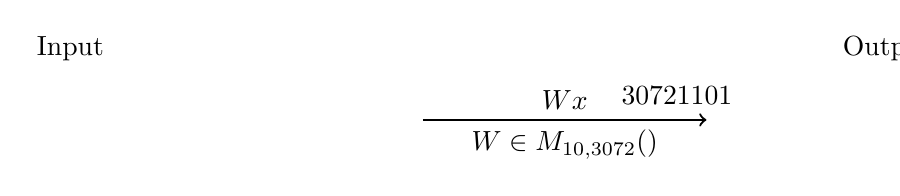
\begin{tikzpicture}
        \node at (-7, 0.7) {Input};
        \parallelepiped{(-4, 0, 0)}{6}{.5}{.5}{$3072$}{$1$}{}{blue!20}

        \draw[->, thick] (-3.4, -.2) -- (0.2, -.2) node[above, pos=.5] {$Wx$} node[below, pos=.5] {$W\in\mathscr{M}_{10,3072}(\R)$};

        \node at (2.5, .7) {Output};
        \parallelepiped{(4, 0, 0)}{3}{.5}{.5}{$10$}{$1$}{}{red!30}
    \end{tikzpicture}
    \caption{Fully-Connected Layer}
\end{figure}

Instead, a CNN takes as an input a 3D volume: for instance, an image can be represented as a tensor of shape $3\times32\times32$, the first dimension being the number of channels (red, green, blue), and the other two being the width and height of the image.

\subsubsection{Kernels}
The convolutional layer itself consists of small kernels (also called filters) used to \emph{convolve} with the image, that is sliding over it spatially, and computing the dot products at each possible location.
\begin{definition}[Kernel]
    A \emph{kernel} (or \emph{filter}) is a tensor of dimensions $D\times K\times K$, where $D$ is the number of channels (or \say{depth}) of the input, and $K$ is a parameter called \emph{kernel size}.
\end{definition}

\begin{definition}[Convolution of two matrices]
    Given two matrices $A=(a_{i, j})_{i, j}$ and $B=(b_{i, j})_{i, j}$ in $\mathscr{M}_{m, n}(\R)$, the \emph{convolution of $A$ and $B$}, noted $A*B\in\R$, is the following:
    \begin{equation}
        A*B = \sum_{i=1}^m \sum_{j=1}^n a_{(m-i+1), (n-j+1)} \cdot b_{i, j}
    \end{equation}
    This corresponds to the dot product in the space $\mathscr{M}_{m, n}(\R)$.
\end{definition}

\begin{definition}[Kernel convolution]
    An input of shape $C\times H\times W$ can be processed by a kernel of shape $C\times K\times K$ by computing at each possible spatial position the convolution between the kernel and the submatrix of the input. 
    \begin{figure}[H]
        \centering
        \begin{tikzpicture}[scale=.5]
            \tdplotsetmaincoords{70}{140}
            \begin{scope}[tdplot_main_coords,canvas is yz plane at x=0]
                \draw[fill=red!50, thick] (19, 8) rectangle (20, 9);
                \draw (18,4) grid (24, 10);

                \draw[thick,dotted] (9,4) -- (19,8);
                \draw[thick,dotted] (9,7) -- (19,9);
                \draw[thick,dotted] (12,4) -- (20,8);
                \draw[thick,dotted] (12,7) -- (20,9);

                \draw[fill=blue!70, fill opacity=.6, thick] (9, 4) rectangle (12, 7);
                \draw (8,0) grid (16, 8);

                \draw[thick,dotted] (0, 0) -- (9, 4);
                \draw[thick,dotted] (0, 3) -- (9, 7);
                \draw[thick,dotted] (3, 0) -- (12, 4);
                \draw[thick,dotted] (3, 3) -- (12, 7);

                \draw[fill=orange, fill opacity=.5, thick] (0,0) rectangle (3, 3);
                \draw (0,0) grid (3, 3);

                \node at (1.5, -1.5) {Kernel};
                \node at (11.5, -1.5) {Input};
                \node at (22, 2.5) {Activation map};
            \end{scope}
        \end{tikzpicture}
        \caption{Kernel convolution}
    \end{figure}
    
    The output of this operation in an \emph{activation map} of dimension $1\times (H - K + 1) \times (W - K + 1)$ representing for each pixel the convolution between the kernel and the corresponding chunk of the image.
    \begin{figure}[H]
        \centering
        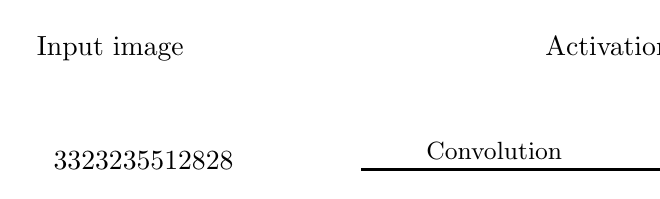
\begin{tikzpicture}[scale=.9]
            \node at (.8, 1.7) {Input image};
            \parallelepiped{(0, 0, 0)}{.5}{4}{3}{$3$}{$32$}{$32$}{blue!20}
            \parallelepiped{(1.3, .3, .3)}{.5}{1.2}{.9}{$3$}{$5$}{$5$}{orange!50}

            \node at (6.7, 1.7) {Activation map};
            \parallelepiped{(6, 0, 0)}{.2}{3.8}{2.8}{$1$}{$28$}{$28$}{red!30}
            \draw[->, thick] (1.8, 0) -- (6.5, 0) node[above, pos=.4] {\small Convolution};

            \parallelepiped{(7.45, .85, 2)}{.15}{.25}{.2}{}{}{}{orange!50}
        \end{tikzpicture}
        \caption{Input and output of the convolution operation}
        \label{fig:one-kernel-layer}
    \end{figure}
\end{definition}

Intuitively, the result of the kernel convolution tells us for each pixel \emph{how much the neighbourhood of the input pixel corresponds to the kernel}.

\begin{example}[Gaussian blur]
    Let $G\in\mathscr{M}_{3}(\R)$ be the following kernel:
    \begin{equation*}
        G := \frac{1}{16}\begin{bmatrix}
            1 & 2 & 1\\
            2 & 4 & 2\\
            1 & 2 & 1
        \end{bmatrix}
    \end{equation*}
    Each coefficient of this matrix is an approximation of the Gaussian distribution. Applying this kernel to an image produces a smoothed version of the input.
\end{example}
% TODO: add gaussian blur image

\begin{example}[Sobel operator]
    Let $S_x$ and $S_y\in\mathscr{M}_{3}(\R)$ be the following kernels:
    \begin{equation*}
        S_x := \begin{bmatrix}
            +1 & 0 & -1\\
            +2 & 0 & -2\\
            +1 & 0 & -1
        \end{bmatrix}
        \qquad\textnormal{and}\qquad
        S_y := S_x^\tp = \begin{bmatrix}
            +1 & +2 & +1\\
            \phantom{+}0 & \phantom{+}0 & \phantom{+}0\\
            -1 & -2 & -1
        \end{bmatrix}
    \end{equation*}
    The convolution between these operators and an image produces horizontal and vertical derivatives approximations of the image pixels.

    \begin{figure}[H]
        \centering
    
        \begin{minipage}{0.4\textwidth}
            \centering
            \caption*{Input image}
            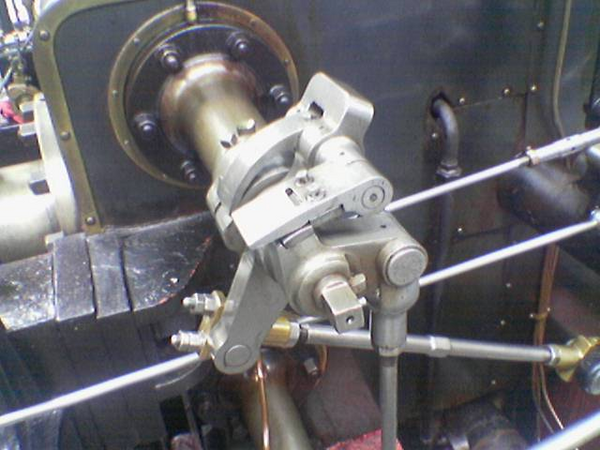
\includegraphics[width=.9\textwidth]{cnn/pre-sobel.png}
        \end{minipage}
        \begin{minipage}{0.4\textwidth}
            \centering
            \caption*{Sobel operator applied to the image}
            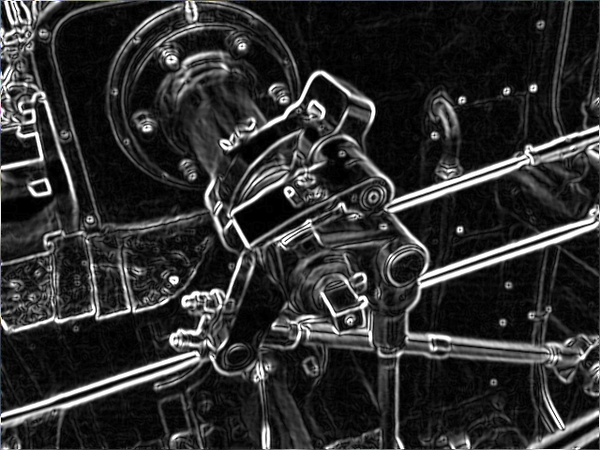
\includegraphics[width=.9\textwidth]{cnn/post-sobel.png}
        \end{minipage}
        
        \caption{Effect of the Sobel operator on an image}
    \end{figure}
\end{example}

These two examples show that kernels used in convolutional layers express meaningful transformations of the input, justifying their use in CNNs. For instance, one could hardcode different kernels (gaussian blur, Sobel operator, vertical/horizontal lines extraction) to extract interesting features from an image, and plug these features into an MLP to obtain an improved classifier compared to a basic, flattening MLP. We will see that instead, CNNs have learnable kernel weights, allowing the model to choose the kernels that it considers bests.

\subsubsection{Multiple kernels}
In Figure \ref{fig:one-kernel-layer}, we used simply one kernel to compute one activation map. In practice, we repeat this process multiple times: we consider a set (or \emph{bank}) of filters having different weights values, and for each kernel of the set, we compute its activation map.
\begin{figure}[H]
    \centering
    \begin{tikzpicture}
        % Input
        \node at (.8, 1.7) {Input image};
        \parallelepiped{(0, 0, 0)}{.5}{4}{3}{$3$}{$32$}{$32$}{blue!20}

        % Convolution Layer
        \draw[thick] (1.5, -1) -- ++ (2.25, 0);
        \node[rectangle,draw,thick,rounded corners] at (5, -1) {\begin{varwidth}{2.5cm}\centering Convolution Layer\end{varwidth}};
        \draw[thick, ->] (6.25, -1) -- ++ (2.25, 0);

        % Kernels
        \node at (5, -4.5) {6 kernels};
        \draw[thick, ->] (5.1, -2.5) -- ++ (0, 0.9);
        \parallelepiped{(3.8, -3, 0)}{.3}{1}{.75}{$3$}{$5$}{}{orange!40};
        \foreach \x in {4.3, 4.8, ..., 5.8} {
            \parallelepiped{(\x, -3, 0)}{.3}{1}{.75}{}{}{}{orange!40};
        }
        \parallelepiped{(6.3, -3, 0)}{.3}{1}{.75}{}{}{$5$}{orange!40};

        % Activation maps
        \node at (10.8, 1.7) {6 activation maps};
        \parallelepiped{(9, 0, 0)}{.2}{3.5}{2.75}{$1$}{$28$}{}{red!40};
        \foreach \x in {9.5, 10, ..., 11} {
            \parallelepiped{(\x, 0, 0)}{.2}{3.5}{2.75}{}{}{}{red!40};
        }
        \parallelepiped{(11.5, 0, 0)}{.2}{3.5}{2.75}{}{}{$28$}{red!40};
        \node at (10.7, -4.5) {$6\times28\times28$ output};
    \end{tikzpicture}
    \caption{Convolutional Layer using 6 kernels}
\end{figure}

Using a bank containing $C'$ filters, the output of the convolutional layer in an \emph{activation map} of dimension $C'\times (H - K + 1) \times (W - K + 1)$ representing for each pixel the convolution between the given kernel and the corresponding chunk of the image.

\begin{remark}[Biases in Convolutional Layers]
    Similarly to fully-connected layers, we often add to the activation map of each kernel a bias of size $1\times (H - K + 1) \times (W - K + 1)$. Those biases might me ommited in the rest of the chapter for the sake of simplicity.
\end{remark}

\subsubsection{Stacking convolutions}
Like previously introduced layers, convolutional layers can be stacked to form deep networks. The layer shapes need to match, in particular the output channels of a layer must match the input channels of the next layer, and the output height and width must match the next input height and width.
\begin{figure}[H]
    \centering
    \begin{tikzpicture}
        % Input
        \node at (.5, 1.9) {\begin{varwidth}{3cm}\centering Input image $3\times32\times32$\end{varwidth}};
        \parallelepiped{(0, 0, 0)}{.5}{4}{3}{$3$}{$32$}{$32$}{blue!20}

        % Convolution layer
        \draw[thick] (1.5, -1) -- ++ (.8, 0);
        \node[rectangle,draw,thick,rounded corners] at (3, -1) {Conv.};
        \draw[thick, ->] (3.7, -1) -- ++ (.8, 0);
        \node at (3, -.3) {$6\times3\times5\times5$};

        % First hidden layer
        \node at (6, 1.7) {\begin{varwidth}{3.5cm}\centering First hidden layer $3\times28\times28$\end{varwidth}};
        \parallelepiped{(5.75, 0, 0)}{1}{3.5}{2.5}{$6$}{$28$}{$28$}{red!40}

        % Convolution layer
        \draw[thick] (7, -1) -- ++ (.8, 0);
        \node[rectangle,draw,thick,rounded corners] at (8.5, -1) {Conv.};
        \draw[thick, ->] (9.2, -1) -- ++ (.8, 0);
        \node at (8.5, -.3) {$10\times6\times3\times3$};

        % Second hidden layer
        \node at (11.5, 1.5) {\begin{varwidth}{4cm}\centering Second hidden layer $3\times26\times26$\end{varwidth}};
        \parallelepiped{(11.5, 0, 0)}{1.3}{3.1}{2.1}{$10$}{$26$}{$26$}{green!20}

        % Convolution layer
        \draw[thick] (12.5, -1) -- ++ (.8, 0);
        \node[rectangle,draw,thick,rounded corners] at (14, -1) {Conv.};
        \draw[thick, ->] (14.7, -1) -- ++ (.8, 0);
        \node at (14, -.3) {$12\times10\times3\times3$};
    \end{tikzpicture}
    \caption{Stacking of 3 Convolutional Layers of correct shapes}
\end{figure}

However, stacking two convolution layers next to each other produces another convolutional layers, and do not add representation power. Therefore, we use the exact same solution as for linear classifiers: we introduce non-linear layers using activation functions in between convolutional layers.
\begin{figure}[H]
    \centering
    \begin{tikzpicture}
        % Input
        \node at (.5, 1.9) {\begin{varwidth}{3cm}\centering Input image $3\times32\times32$\end{varwidth}};
        \parallelepiped{(0, 0, 0)}{.5}{4}{3}{$3$}{$32$}{$32$}{blue!20}

        % Convolution layer
        \draw[thick] (1.2, -1) -- ++ (.35, 0);
        \draw[thick] (2.85, -1) -- ++ (.2, 0);
        \draw[thick, ->] (4.35, -1) -- ++ (.5, 0);
        \node[rectangle,draw,thick,rounded corners] at (2.2, -1) {Conv.};
        \node[rectangle,draw,thick,rounded corners] at (3.7, -1) {ReLU};

        % First hidden layer
        \node at (6, 1.7) {\begin{varwidth}{3.5cm}\centering First hidden layer $3\times28\times28$\end{varwidth}};
        \parallelepiped{(5.75, 0, 0)}{.8}{3.5}{2.5}{$6$}{$28$}{$28$}{red!40}

        % Convolution layer
        \draw[thick] (6.8, -1) -- ++ (.35, 0);
        \draw[thick] (8.45, -1) -- ++ (.2, 0);
        \draw[thick, ->] (9.95, -1) -- ++ (.5, 0);
        \node[rectangle,draw,thick,rounded corners] at (7.8, -1) {Conv.};
        \node[rectangle,draw,thick,rounded corners] at (9.3, -1) {ReLU};

        % Second hidden layer
        \node at (11.5, 1.5) {\begin{varwidth}{4cm}\centering Second hidden layer $3\times26\times26$\end{varwidth}};
        \parallelepiped{(11.5, 0, 0)}{1}{3.1}{2.1}{$10$}{$26$}{$26$}{green!20}

        % Convolution layer
        \draw[thick] (12.5, -1) -- ++ (.35, 0);
        \draw[thick] (14.15, -1) -- ++ (.2, 0);
        \draw[thick, ->] (15.65, -1) -- ++ (.5, 0);
        \node[rectangle,draw,thick,rounded corners] at (13.5, -1) {Conv.};
        \node[rectangle,draw,thick,rounded corners] at (15, -1) {ReLU};
    \end{tikzpicture}
    \caption{Adding ReLU layers in between Convolution Layers}
\end{figure}

\subsubsection{Spatial dimensions and Padding}
As stated previously, using an input of width $W$ with a filter of kernel size $K$, the output width is $W-K+1$. A problem with the approach is that features maps decrease in size with each layer. This creates an upper bound on the maximum number of layers that we can use for our model. 

A solution to this is to introduce \emph{padding} by adding zeros around the border of the input. When the kernel will slide around the edges of the input, a part of the coefficients that it will consider in its convolution will be zeros.
\begin{figure}[H]
    \centering
    \begin{tikzpicture}
        \newcommand{\randint}{
            \pgfmathsetmacro{\temp}{random(0, 9)}
            \temp
        }
        \newcommand{\phant}{
            \makebox[0pt][l]{\footnotesize\,$\cdot$}\phantom{0}
        }

        \tikzstyle{number matrix}=[
            matrix of math nodes,
            nodes={
                minimum size=1em, 
                outer sep=0pt,
                inner sep=0,line
                width=0.5pt,
            },
            nodes in empty cells,
            column sep=-0.5pt,
            row sep=-0.5pt
        ]
        
        \matrix [number matrix, nodes={
            append after command={
                \pgfextra{\draw[thick, dashed]
                ($(\tikzlastnode.north west)+(-0.3em,+0.3em)$)
                rectangle ($(\tikzlastnode.south east)+(0.3em,-0.3em)$);}
            }
        }] at (0, 0)
        {
            0 & 0 & 0 & 0 & 0 & 0 & 0 & 0 \\
            0 & 0 & 0 & 0 & 0 & 0 & 0 & 0 \\
            0 & 0 & 0 & 0 & 0 & 0 & 0 & 0 \\
            0 & 0 & 0 & 0 & 0 & 0 & 0 & 0 \\
            0 & 0 & 0 & 0 & 0 & 0 & 0 & 0 \\
            0 & 0 & 0 & 0 & 0 & 0 & 0 & 0 \\
            0 & 0 & 0 & 0 & 0 & 0 & 0 & 0 \\
            0 & 0 & 0 & 0 & 0 & 0 & 0 & 0 \\
        };

        \matrix [number matrix, nodes={
            append after command={
                \pgfextra{\draw[thick, fill=gray!30]
                ($(\tikzlastnode.north west)+(-0.3em,+0.3em)$)
                rectangle ($(\tikzlastnode.south east)+(0.3em,-0.3em)$);}
            }
        }] at (0, 0)
        {
            2 & 5 & \randint & \randint & \randint & \randint \\
            7 & 1 & \randint & \randint & \randint & \randint \\
            \randint & \randint & \randint & \randint & \randint & \randint \\
            \randint & \randint & \randint & \randint & \randint & \randint \\
            \randint & \randint & \randint & \randint & \randint & \randint \\
            \randint & \randint & \randint & \randint & \randint & \randint \\
        };

        \fill[color=blue, fill opacity=.4] (-8/3, 8/3) rectangle (-2/3, 2/3);

        % Dashed connections
        \draw[-, dashed] (-8/3, 8/3) -- (4, 1);
        \draw[-, dashed] (-2/3, 8/3) -- (6, 1);
        \draw[-, dashed] (-8/3, 2/3) -- (4, -1);
        \draw[-, dashed] (-2/3, 2/3) -- (6, -1);

        \draw[-, dashed] (4, 1) -- (8, 2);
        \draw[-, dashed] (6, 1) -- (26/3, 2);
        \draw[-, dashed] (4, -1) -- (8, 4/3);
        \draw[-, dashed] (6, -1) -- (26/3, 4/3);

        \matrix [number matrix, nodes={
            append after command={
                \pgfextra{\draw[thick, fill=orange, fill opacity=.6]
                ($(\tikzlastnode.north west)+(-0.3em,+0.3em)$)
                rectangle ($(\tikzlastnode.south east)+(0.3em,-0.3em)$);}
            }
        }] at (5, 0)
        {
            \randint & \randint & \randint \\
            \randint & 1 & 1 \\
            \randint & 0 & 2 \\
        };

        \fill[color=red, fill opacity=.5] (8, 2) rectangle (26/3, 4/3);
        \matrix [number matrix, nodes={
            append after command={
                \pgfextra{\draw[thick]
                ($(\tikzlastnode.north west)+(-0.3em,+0.3em)$)
                rectangle ($(\tikzlastnode.south east)+(0.3em,-0.3em)$);}
            }
        }] at (10, 0)
        {
            9 & \phant & \phant & \phant & \phant & \phant \\
            \phant & \phant & \phant & \phant & \phant & \phant \\
            \phant & \phant & \phant & \phant & \phant & \phant \\
            \phant & \phant & \phant & \phant & \phant & \phant \\
            \phant & \phant & \phant & \phant & \phant & \phant \\
            \phant & \phant & \phant & \phant & \phant & \phant \\
        };

        \node at (3.3, 0) {\Large *};
        \node at (6.9, 0) {\Large =};

        \node at (0, 3.2) {Input image with $(1, 1)$ padding};
        \node at (0, -3.2) {$6\times6 \longrightarrow 8\times8$};
        \node at (5, -1.5) {$3\times3$};
        \node at (10, 2.5) {Output image};
        \node at (10, -2.5) {$6\times6$};

    \end{tikzpicture}
    \caption{Adding padding around the input}
\end{figure}

\begin{remark}[Padding strategies]
    Even though we might imagine different padding strategies instead of always padding with zeros (for instance, nearest-neightbour padding, circular padding, random padding\dots), zero-padding seems to be both simple and effective in practice, and is the most commonly used strategy.
\end{remark}

Padding introduces an additional hyperparameter to the layer, $P$. 
Using padding, the width of the output of the layer becomes:
\begin{equation}
    \label{eq:output-padding}
    W'=W-K+2P+1
\end{equation}
A common way to set the value of $P$ is to choose it such as the output have the same size as the input. This is achieved by taking $P=(K-1)/2$, called \emph{same-padding}. This is only possible if $K$ is odd, which is often the case in practice, since same-padding is often the expected behavior.

\subsubsection{Receptive Fields}
\begin{definition}[Receptive Field]
    The \emph{receptive field} of an output neuron is the set of neurons of the input of which the output neuron depends on.
\end{definition}

By essence, Fully-connected layers have a trivial notion of receptive field: an output neuron is connected to each input neuron, its receptive field is therefore the entire input.

Convolution layers are build in such a way that each element in the output simply depends on a receptive field of size $K$ (that is a square of area $K\times K$) in the input. As we stack convolutional layers after the others, each successive convolution adds $K-1$ to the receptive field size. After $L$ layers, the receptive field size is $1+L\times(K-1)$. 

\begin{figure}[H]
    \centering
    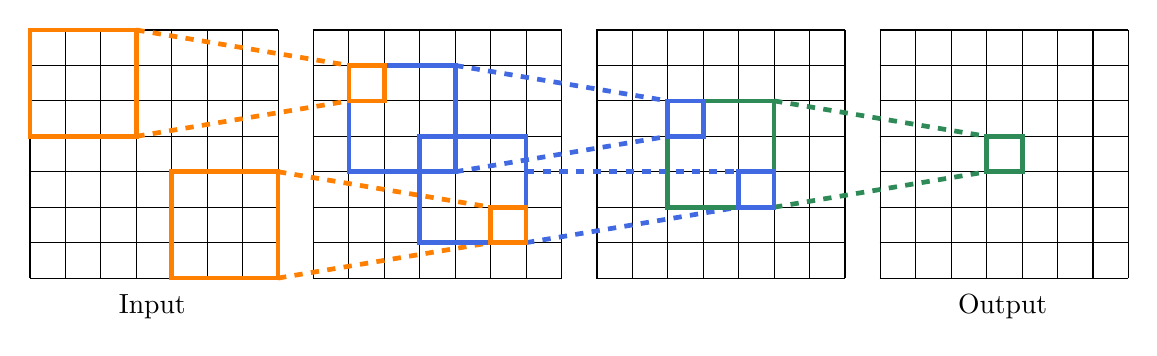
\begin{tikzpicture}[scale=.9]
        \tikzstyle{custom width}=[line width=0.6mm]
        \tikzstyle{orange}=[color=orange]
        \tikzstyle{blue}=[color=RoyalBlue]
        \tikzstyle{green}=[color=SeaGreen]

        \draw[step=0.5] (0,0) grid (3.5,3.5);
        \node at (1.725, -.4) {Input};
        \draw[step=0.5] (3.99,0) grid (7.5,3.5);
        \draw[step=0.5] (7.99,0) grid (11.5,3.5);
        \draw[step=0.5] (11.99,0) grid (15.5,3.5);
        \node at (13.725, -.4) {Output};

        \draw[orange, custom width] (0,2) rectangle ++(1.5,1.5);
        \draw[orange, dashed, custom width] (1.5, 3.5) -- (4.5,3);
        \draw[orange, dashed, custom width] (1.5, 2) -- (4.5,2.5);

        \draw[orange, custom width] (2,0) rectangle ++(1.5,1.5);
        \draw[orange, dashed, custom width] (3.5, 1.5) -- (6.5,1);
        \draw[orange, dashed, custom width] (3.5, 0) -- (6.5,.5);

        \draw[blue, custom width] (4.5,1.5) rectangle ++(1.5,1.5);
        \draw[blue, dashed, custom width] (6,3) -- (9,2.5);
        \draw[blue, dashed, custom width] (6,1.5) -- (9,2);

        \draw[blue, custom width] (5.5,0.5) rectangle ++(1.5,1.5);
        \draw[blue, dashed, custom width] (7,1.5) -- (10,1.5);
        \draw[blue, dashed, custom width] (7,0.5) -- (10,1);

        \draw[orange, custom width] (4.5,2.5) rectangle ++(.5,.5);
        \draw[orange, custom width] (6.5,0.5) rectangle ++(.5,.5);

        \draw[green, custom width] (9,1) rectangle ++(1.5,1.5);
        \draw[green, dashed, custom width] (10.5,2.5) -- (13.5,2);
        \draw[green, dashed, custom width] (10.5,1) -- (13.5,1.5);

        \draw[blue, custom width] (9,2) rectangle ++(.5,.5);
        \draw[blue, custom width] (10,1) rectangle ++(.5,.5);

        \draw[green, custom width] (13.5,1.5) rectangle ++(.5,.5);
    \end{tikzpicture}
    \caption{Receptive field of an output neuron}
\end{figure}

This linear growth shows that by stacking enough layers, each output neuron will eventually have the entire input image in its receptive field. Nevertheless, this can be a problem in practice as we might need many layers for each output to depend on the whole image.

A solution to this problem is to downsample the image size inside the network. This can be done by adding another hyperparameter, \emph{stride}.

\subsubsection{Strided Convolution}
\begin{definition}[Stride]
    The hyperparameter \emph{stride} defines the number of pixels between two applications of the kernel.
\end{definition}
\begin{wrapfigure}{r}{0.4\textwidth}
    \centering
    \begin{tikzpicture}
        \newcommand{\randint}{
            \pgfmathsetmacro{\temp}{random(0, 1)}
            \temp
        }
        \fill[orange!60] (-2, -2) rectangle (2, 2);
        \matrix [
            matrix of math nodes,
            nodes={
                minimum size=1em, 
                outer sep=0pt,
                inner sep=0,line
                width=0.5pt,
                append after command={
                    \pgfextra{\draw[thick] 
                    ($(\tikzlastnode.north west)+(-0.3em,+0.3em)$)
                    rectangle ($(\tikzlastnode.south east)+(0.3em,-0.3em)$);}
                }
            },
            nodes in empty cells,
            column sep=-0.5pt,
            row sep=-0.5pt
        ]
        {
            \randint & \randint & \randint & \randint & \randint & \randint \\
            \randint & \randint & \randint & \randint & \randint & \randint \\
            \randint & \randint & \randint & \randint & \randint & \randint \\
            \randint & \randint & \randint & \randint & \randint & \randint \\
            \randint & \randint & \randint & \randint & \randint & \randint \\
            \randint & \randint & \randint & \randint & \randint & \randint \\
        };

        \draw[densely dashed, color=red, line width=1mm] (-2, 0) rectangle (0, 2);
        \draw[color=red, line width=1mm] (-2/3, 0) rectangle (4/3, 2);

        \draw[<->, color=red, very thick] (-2, 2.2) -- (-2/3, 2.2) node[above, pos=.5] {\bf stride};
    \end{tikzpicture}
    \caption{Effect of stride}
\end{wrapfigure}

Stride effectively downsamples the size of the image. Applying a convolution between an image of width $W$ and padding $P$ with a kernel of size $K$ and stride $S$ produces the following output dimension:
\begin{equation}
    \label{eq:output-stride}
    W'=\frac{W-K+2P}{S}+1
\end{equation}
Note that choosing $S=1$ in \eqref{eq:output-stride} gives the same result as \eqref{eq:output-padding}. Depending on the implementation, the result can be rounded up or down in the case where it is not an integer. Usually, all the parameters are chosen such that $S$ divides $W-K+2P$.

\subsection{Pooling Layers}
\subsubsection{Introduction}
Computer Vision, one of the most frequent use for CNNs, often deals with images of high quality, making downsampling an important task to drastically reduce the number of layers and the quantity of VRAM used by the model. We saw a first approach to downsampling embedded in Convolutional Layers, that is strided convolution. Pooling Layers are layers dedicated to downsampling, without learnable parameters.

Pooling layers work similarly to convolutional layers, using a mechanism of kernels. Nevertheless, instead of applying a convolution between some kernel and the image, the layer will apply a pooling function to the area of the input. This will produce an activation map with dimensions depending on the hyperparameters of the layer -- kernel size, padding and stride, the same as the parameters of a convolutional layer.

\begin{figure}[H]
    \centering
    \begin{tikzpicture}
        % Left block
        \parallelepiped{(0, 0, 0)}{2}{3}{2.5}{$64$}{$224$}{$224$}{orange!70};
        \parallelepiped{(-1.5, 0, 0)}{.15}{3}{2.5}{1}{}{}{blue!50};
        \draw[thick] (-2,0) -- ++(2, 0);

        % Right block
        \parallelepiped{(7, -.5, 0)}{2}{1.5}{1.5}{$64$}{$112$}{$112$}{orange!70};
        \parallelepiped{(5.5, -.5, 0)}{.15}{1.5}{1.5}{1}{}{}{blue!50};
        \draw[thick] (5,-.5) -- ++(2, 0);

        % Pooling arrow
        \draw[thick, ->] (1.5, -1.2) -- ++(2.2, 0) node[pos=.5, above] {Pooling};
        % Downsampling arrow
        \draw[thick, ->] (0.2, -6.5) -- ++(4.3, 0) node[pos=.5, above] {Downsampling};
        
        % Left image
        \draw[thick, ->] (-1.5, -3.8) -- ++(0,-1);
        \node at (-1.5, -6.5) {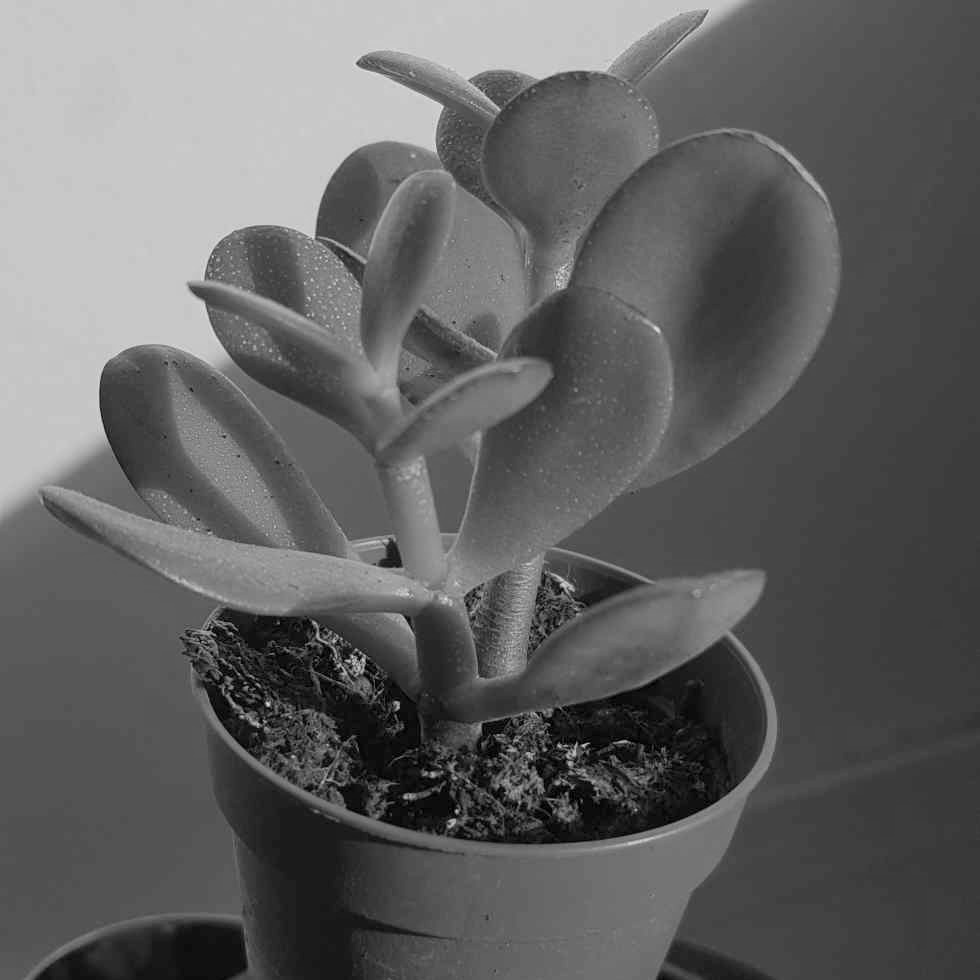
\includegraphics[width=80pt]{cnn/plante.jpg}};
        \node at (-3.3, -6.5) {$224$};
        \node at (-1.5, -8.2) {$224$};
        
        % Right image
        \draw[thick, <-] (5.5, -2.8) -- ++(0,-2.8);
        \node at (5.5, -6.5) {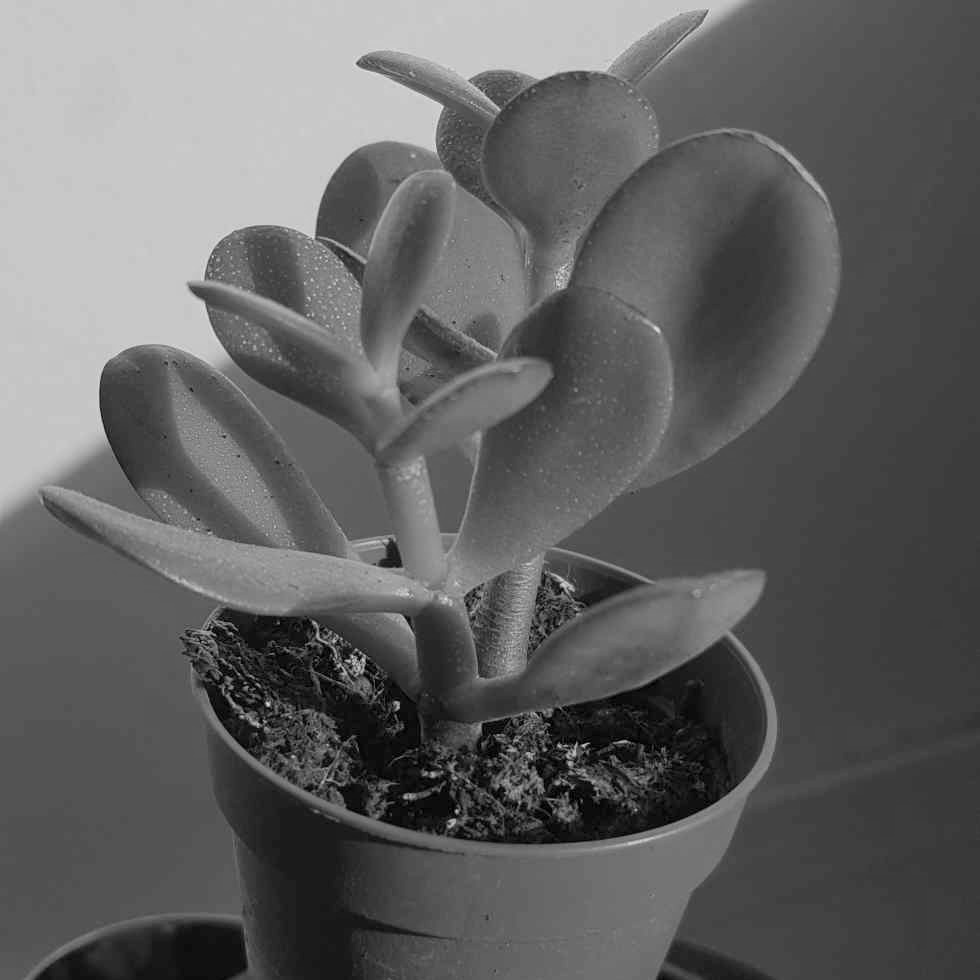
\includegraphics[width=40pt]{cnn/plante.jpg}};
        \node at (6.6, -6.5) {$112$};
        \node at (5.5, -7.5) {$112$};
    \end{tikzpicture}
    \caption{Behavior of a pooling layer}
\end{figure}
Another difference is that the operation is applied for each slice of the input volume. Choosing appropriate values for the hyperparameters (for instance $S\geq2$, \dots) allow to downsample the input without the need for learnable parameters.

\subsubsection{Max Pooling}
\begin{definition}[Max Pooling function]
    For $K\geq 1$, the \emph{Max Pooling function} of kernel size $K$ is:
    \begin{equation*}
        \begin{aligned}
            \textnormal{max}_P: \mathscr{M}_{K}(\R) &\longrightarrow \R\\
            (m_{i, j}) &\longmapsto \max_{i, j} m_{i, j}
        \end{aligned}
    \end{equation*}
\end{definition}

A \emph{Max Pooling} layer applies the Max Pooling function to each location of size $K\times K$ in each slice of the input volume. We often choose the same kernel size as the slide (that is $K=S$) to avoid recovering twice the same pixel value. In this setting, it is equivalent to spliting each input channel into non-overlapping regions of size $K\times K$, from which are extracted the maximum value of the section and stored in the output channel.

Max Pooling has some advantages over convolutional layers with stride: it does not involve learnable parameters, reducing the computational cost, but also introduces translational invariance to small spatial shifts. Indeed, if the position of a specific maximum pixel is moved slightly, we might intuitively think that it will stay the maximum of its region, making the model robust to small translations.

\subsubsection{Average Pooling}
\begin{definition}[Average Pooling function]
    For $K\geq 1$, the \emph{Average Pooling function} of kernel size $K$ is:
    \begin{equation*}
        \begin{aligned}
            \textnormal{avg}_P: \mathscr{M}_{K}(\R) &\longrightarrow \R\\
            (m_{i, j}) &\longmapsto \frac{1}{K^2}\sum_{i=1}^K \sum_{j=1}^K m_{i, j}
        \end{aligned}
    \end{equation*}
    It simply returns the average of the matrix coefficients.
\end{definition}

Average Pooling works exactly the same as Max Pooling, but applying $\textnormal{avg}_P$ as a pooling function instead of $\textnormal{max}_P$.

\subsection{A full CNN example: LeNet-5}
Now that we have these different types of layers, we can stack them together to create a full CNN architecture. A classic model often fits the following architecture:
\begin{equation*}
    (\texttt{Conv, ReLU, Pooling})^{N_1} \rightarrow \texttt{Flatten} \rightarrow (\texttt{Linear, ReLU})^{N_2} \rightarrow \texttt{Linear}
\end{equation*}

As an example, we will take the 1998 model \emph{LeNet-5}:
\begin{figure}[H]
    \centering
    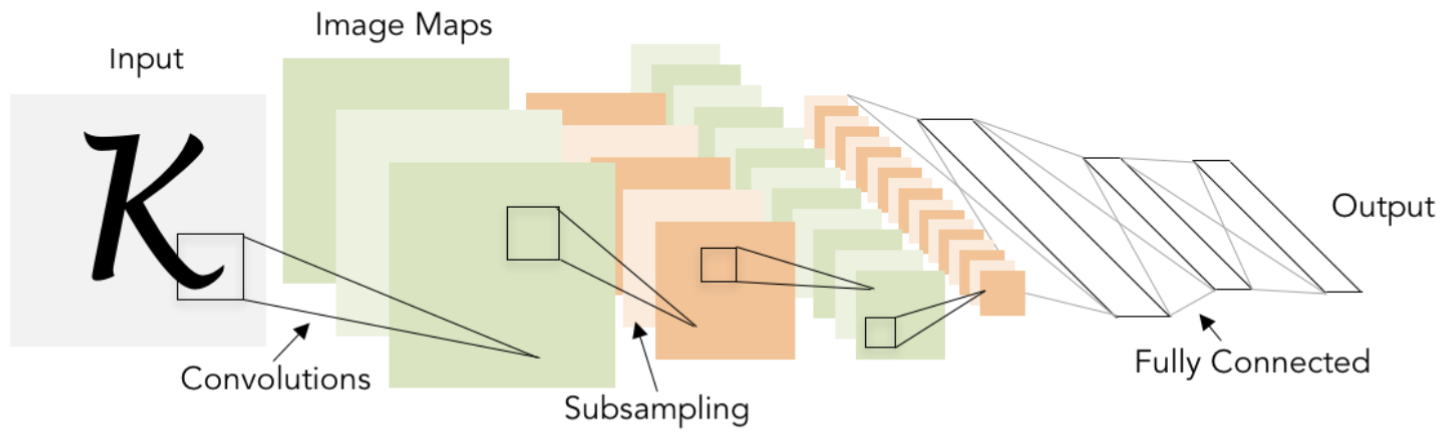
\includegraphics[width=0.8\textwidth]{cnn/lenet-5.png}
    \caption{LeNet-5 architecture}
\end{figure}
The first blocks of Convolutional and Pooling layers progressively decrease the spatial size of the input, while increasing the number of channels: the total volume of the input is preserved.

\subsection{Normalization}
Deep convolutional neural networks are described previously can be extremly effective when trained; nevertheless, they are also very difficult to train, and we need to properly prepare data for the descent to converge.

A recent solution to ease the training is to add \emph{normalization layers} in the network.

\subsubsection{Batch Normalization}
The idea of Batch Normalization is to normalize the outputs of a layer, often by giving the output a zero mean and unit variance. This improves optimization by guaranteeing that a layer always receive similar data from the previous layer's output. Indeed, while training, the distribution of the output of a layer might change, which tends to increase the complexity of the learning process. In contrast, the output of a batch normalization layers always has the same mean and variance; therefore, the next layer can always \say{see} the same input data distribution, improving convergence.

Normalizing batches of activations can simply be implemented using the following formula:
\begin{equation*}
    \hat{x}^{(k)} := \frac{x^{(k)} - \E[x^{(k)}]}{\sqrt{\V[x^{(k)}]}}
\end{equation*}
Hopefully, this is a differentiable function, and can therefore be seen as any other layer in the network, and implement its backward gradient.

\subsubsection{Batch Normalization in practice}
Consider a fully-connected setup, in which we have a batch $x$ consisting of $N$ inputs, each of size $D$. We will use the $N$ batch samples to compute the empirical mean for each of the element of the $D$-shaped vector:
\begin{equation*}
    \mu_j := \frac{1}{N}\sum_{i=1}^N x_{i, j}
\end{equation*}
which gives us a vector $\mu$ of size $D$. Similarly, the standard deviation of the batch can be computed element-wise:
\begin{equation*}
    \sigma_j^2 := \frac{1}{N}\sum_{i=1}^N (x_{i,j}-\mu_j)^2
\end{equation*}
giving us a vector $\sigma$ of size $D$ as well. Finally, each element of the batch $x$ is normalized, giving us $\hat{x}$:
\begin{equation*}
    \hat{x}_{i,j} := \frac{x_{i,j}-\mu_j}{\sqrt{\sigma^2_j+\epsilon}}
\end{equation*}
The small constant $\epsilon$ is added at the denominator to avoid diving by zero when the standard deviation is null.

In practice, zero mean and unit variance can be too hard of a constraint on the network. We prefer to add learnable scale and shift parameters $\gamma$ and $\beta$ of size $D$, allowing the network to choose what mean and variance it wants for the next layer. The acutal output is therefore $y$, defined by:
\begin{equation*}
    y_{i,j} := \gamma_j\hat{x}_{i,j}+\beta_j
\end{equation*}
Note that learning $\gamma=\sigma$ and $\beta=\mu$ recovers the identity function, making the network able to bypass the normalization layer if it is not needed.

An important note is that batch normalization introduces dependence on the minibatches: previously, each image in the input batch was handled independently of the others, which is not the case anymore with batch normalization. We cannot do this at test time, since it would not guarantee the reproducibility of classification, and more importantly, it would be a security breach to make each classification depend on the other inputs. To avoid this, batch normalization layers behave differently during training and testing. During training, the layer normalizes the batches as described before, while maintaining the empirical mean and variance of the inputs, $\mu$ and $\sigma$. These empirical vectors learned during training are then treated as constants and used during testing to normalize the test inputs.

Hence, at test time, the normalization layer performs the following operation:
\begin{equation*}
    y = \gamma\cdot\frac{x-\mu}{\sigma}+\beta
\end{equation*}
Another interesting property of this method is that during testing, the batch normalization layer becomes a linear operator. Therefore, it can be fused with the previous fully-connected or convolutional layer. For instance, if the previous layer is a fully-connected, its weight matrix and bias vector can be modified using the four parameters of the normalization layer (learned mean and variance, and empirical mean and variance). Performing this operation guarantees that the batch normalization layer does not add any inference time. 

\subsubsection{Batch Normalization for Convolutional Networks}
For fully-connected layers, the batch dimension is:
\begin{equation*}
    x: N\times D
\end{equation*}
Therefore, the batch normalization parameters are the following:
\begin{equation*}
    \begin{cases*}
        \mu, \sigma: 1\times D & (empirical mean and standard deviation)\\
        \gamma, \beta: 1\times D & (learned mean and standard deviation)
    \end{cases*}
\end{equation*}

This needs to be adapted for convolutional layers, but remains very similar. The batch dimension is:
\begin{equation*}
    x: N\times C\times H\times W
\end{equation*}
Instead of averaging only over the batch elements, we will also average over both spacial dimensions. This means that we will take for each channel the average and standard deviation taking into account all the pixels of all the images in the batch. Therefore, the batch normalization parameters are the following:
\begin{equation*}
    \begin{cases*}
        \mu, \sigma: 1\times C\times 1\times 1 & (empirical mean and standard deviation)\\
        \gamma, \beta: 1\times C\times 1\times 1 & (learned mean and standard deviation)
    \end{cases*}
\end{equation*}
which can also be seen as vectors of size $C$; it is nevertheless more convenient to see them in tensor form, $1\times C\times 1\times 1$.

\subsubsection{Advantages and downsides of batch normalization}
As stated previously, adding batch normalization in neural networks allows for models to train much faster, while adding no overhead at testing time when placed after fully-connected or convolutional layers.

Not only the models converge quicker at fixed learning rate, but it also stabilizes the model even with higher learning rates, allowing shorter training times without the risk of divergence.

While they are widely used in practice, normalization layers also come with downsides: the reason of the effectiveness of batch normalization is not well-understood theoretically, and it introduces complex code because of the distinction between training and testing. This is actually a very common source of bugs in projects: one have to remember to change the mode from training to testing. 

Finally, batch normalization is not always appropriate: some very unbalanced data sets might not fit appropriately with batch normalization, and this can reduce the performance of the model. This depends highly on the application: for computer vision, batch normalization is most of the time suitable.

\subsubsection{Layer and Instance normalizations}
A variant to batch normalization, called \emph{layer normalization}, has be proposed. It aims at unifying the behavior of the normalization layer at training and testing time. This guarantees, even at training time, the independence between elements of one batch. The idea is to normalize the input in the layer direction instead of the batch direction. For a fully-connected layer with batch dimension:
\begin{equation*}
    x:N\times D
\end{equation*}
the layer normalization parameters become:
\begin{equation*}
    \begin{cases*}
        \mu, \sigma: N\times 1 & (empirical mean and standard deviation)\\
        \gamma, \beta: \;\,1\times D & (learned mean and standard deviation)
    \end{cases*}
\end{equation*}
This kind of normalization is currently used in recurrent neural networks (RNNs) and transformers.

The equivalent of layer normalization for convolutional layers is called \emph{instance normalization}: similarly, instead of averaging over both the batch and spatial dimensions, we will only normalize over the spatial dimensions. For a convolution layer with batch dimension:
\begin{equation*}
    x: N\times C\times H\times W
\end{equation*}
the layer normalization parameters become:
\begin{equation*}
    \begin{cases*}
        \mu, \sigma: N\times C\times 1\times 1 & (empirical mean and standard deviation)\\
        \gamma, \beta: \;\,1\times C\times 1\times 1 & (learned mean and standard deviation)
    \end{cases*}
\end{equation*}

\begin{figure}[H]
    \centering
    \begin{tikzpicture}[scale=1.3]
        \node at (.6, 2.4) {\bf Batch Norm};
        \node[rotate=90] at (-1.2,0.1) {H, W};
        \node at (0,-1.2) {C};
        \node at (1.7,-0.7) {N};

        \node at (4.6, 2.4) {\bf Layer Norm};
        \node[rotate=90] at (4-1.2,0.1) {H, W};
        \node at (4+0,-1.2) {C};
        \node at (4+1.7,-0.7) {N};

        \node at (8.6, 2.4) {\bf Instance Norm};
        \node[rotate=90] at (8-1.2,0.1) {H, W};
        \node at (8+0,-1.2) {C};
        \node at (8+1.7,-0.7) {N};
        

        \foreach\x in {0, 0.35, ..., 2.1} {
        \foreach\y in {0, 0.35, ..., 2.1} {
        \foreach\z in {0, 0.35, ..., 2.1} {
            % Batch Norm
            \pgfmathparse{\x>=1.75}
            \ifnum\pgfmathresult=1
                \parallelepiped{(\x, \y, \z)}{.3}{.3}{.3}{}{}{}{NavyBlue!100}
            \else
                \parallelepiped{(\x, \y, \z)}{.3}{.3}{.3}{}{}{}{gray!30}
            \fi


            % Layer Norm
            \pgfmathparse{\z>=1.75}
            \ifnum\pgfmathresult=1
                \parallelepiped{(4+\x, \y, \z)}{.3}{.3}{.3}{}{}{}{NavyBlue!100}
            \else
                \parallelepiped{(4+\x, \y, \z)}{.3}{.3}{.3}{}{}{}{gray!30}
            \fi


            % Instance Norm
            \pgfmathparse{\x>=1.75 && \z>=1.75}
            \ifnum\pgfmathresult=1
                \parallelepiped{(8+\x, \y, \z)}{.3}{.3}{.3}{}{}{}{NavyBlue!100}
            \else
                \parallelepiped{(8+\x, \y, \z)}{.3}{.3}{.3}{}{}{}{gray!30}
            \fi
        }}}
    \end{tikzpicture}
    \caption{Visualization of the different types of normalization. The blue squares represent the parts normalized together.}
\end{figure}
\section{Recurrent Neural Networks}
\subsection{Processing Sequences}
So far, all the deep neural networks that we studied (MLPs, CNNs) had the same \emph{feed-forward} global structure: the network receives an input of fixed size, which is fed into the successive layers of the network, which produces a fixed-size output. This is known as a \emph{one-to-one} model, and is mostly used for image classification.

When considering other applications, we would like more flexibility on the input and output sizes. For image captioning, we would like a \emph{one-to-many} model, where the input is a fixed size image, and the output a sentence of variable length. For text classification, such as sentiment analysis, we would like a \emph{many-to-one} model, where the input is a sentence of variable length and the output a fixed-size vector of class probabilities. Finally, we might want both the input and output to be variable in length, for instance in the case of machine translation: this requires a \emph{many-to-many} model.

\begin{figure}[H]
    \centering
    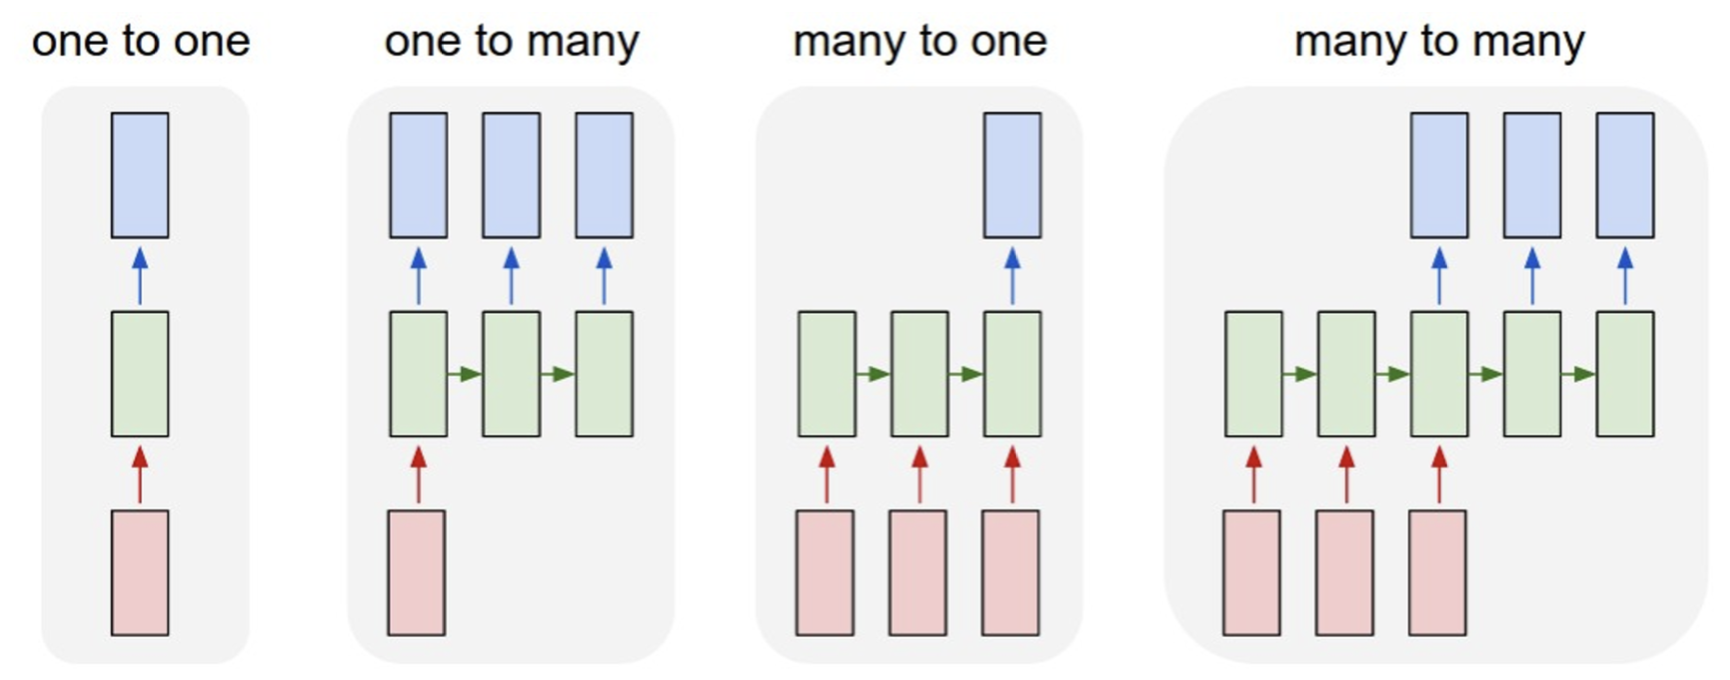
\includegraphics[width=.8\textwidth]{rnn/sequences.png}
\end{figure}

\emph{Recurrent Neural Networks} (RNNs) is a general paradigm which allows to handle all these different setups.

\subsection{Simple Recurrent Neural Network}
\subsubsection{General form}
\begin{wrapfigure}{r}{0.2\textwidth}
    \centering
    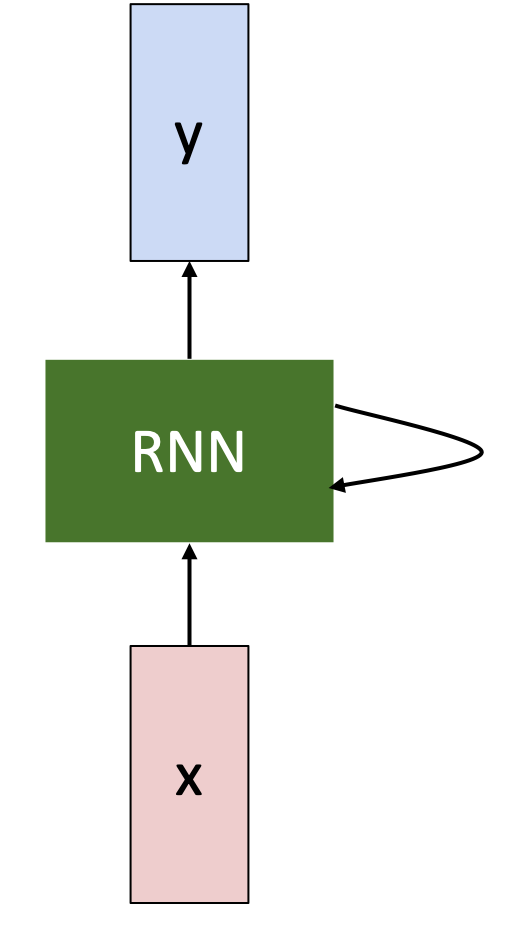
\includegraphics[width=.2\textwidth]{rnn/vanilla-rnn.png}
    \caption{A simple RNN.}
\end{wrapfigure}
In its simplest form, a Recurrent Neural Network posesses an internal hidden state which is updated each time that it reads an input. The handling of a sequential input (for instance, a sentence) follows this update loop: a fixed-size bit of the input is fed into the network, and is combined with the internal hidden state to produce an output and update the state. The next bit of the input is then fed to the network, and so on.

Formally, this can be written as a recurrence relationship:
\begin{equation*}
    h_t = f_W(h_{t-1}, x_t)
\end{equation*}
where $x$ is a sequence of vectors, $(h_t)_t$ is the sequence of hidden states, and $f_W$ is our network depending on some parameter $W$. To produce an output at each time step, we can simply transform the hidden state into an ouput using a feed-forward neural network:
\begin{equation*}
    y_t = g_{W'}(h_t)
\end{equation*}
Note that the same functions $f, g$ and the same parameters $W, W'$ are used at each step, only the internal state changes.

\subsubsection{A vanilla RNN}
We can create a simple RNN built around a single hidden vector $h_t$:
\begin{equation*}
    \begin{aligned}
        h_t &= \tanh\left(W_h h_{t-1} + W_x x_t\right)\\
        y_t &= W_y h_t
    \end{aligned}
\end{equation*}

\subsubsection{Computational graphs of RNNs}
Alongside with this intuition of RNNs as networks with hidden cells, it is also useful to think of RNNs as computational graphs. The graph of an RNN can be unfolded over multiple time steps, expliciting the inputs and gradient flow.
\begin{figure}[H]
    \centering
    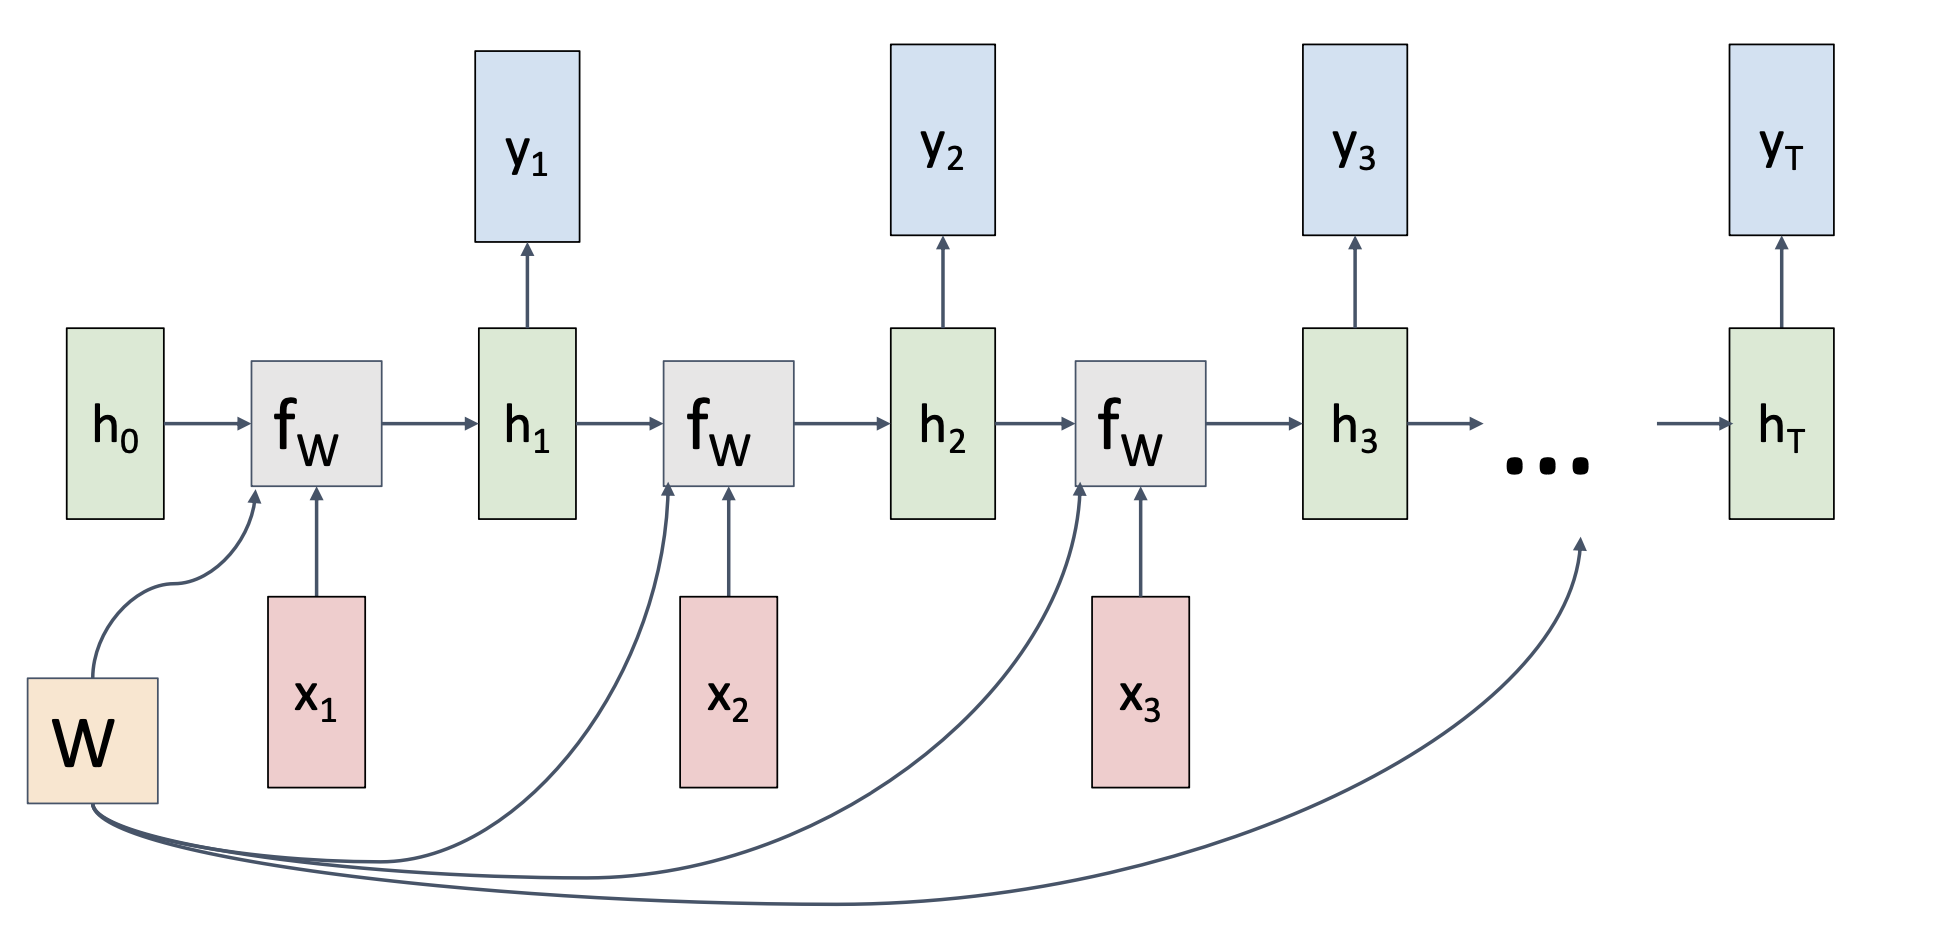
\includegraphics[width=.7\textwidth]{rnn/rnn-graph.png}
    \caption{Unfolded computational graph of an RNN.}
\end{figure}
The initial hidden state $h_0$ is often initialized to 0 in most contexts. It is then fed to the $f_W$ function with the first input $x_1$, which produces the new hidden state $h_1$. This hidden state can be used to compute the output $y_1$.

Note that the parameter $W$ remains the same for all; when computing the gradient $\frac{\partial\L}{\partial W}$, we will sum all the graidents coming from each time step to compute the total gradient.

This unfolded view also allows to understand the relationship with the loss more explicitely.
\begin{figure}[H]
    \centering
    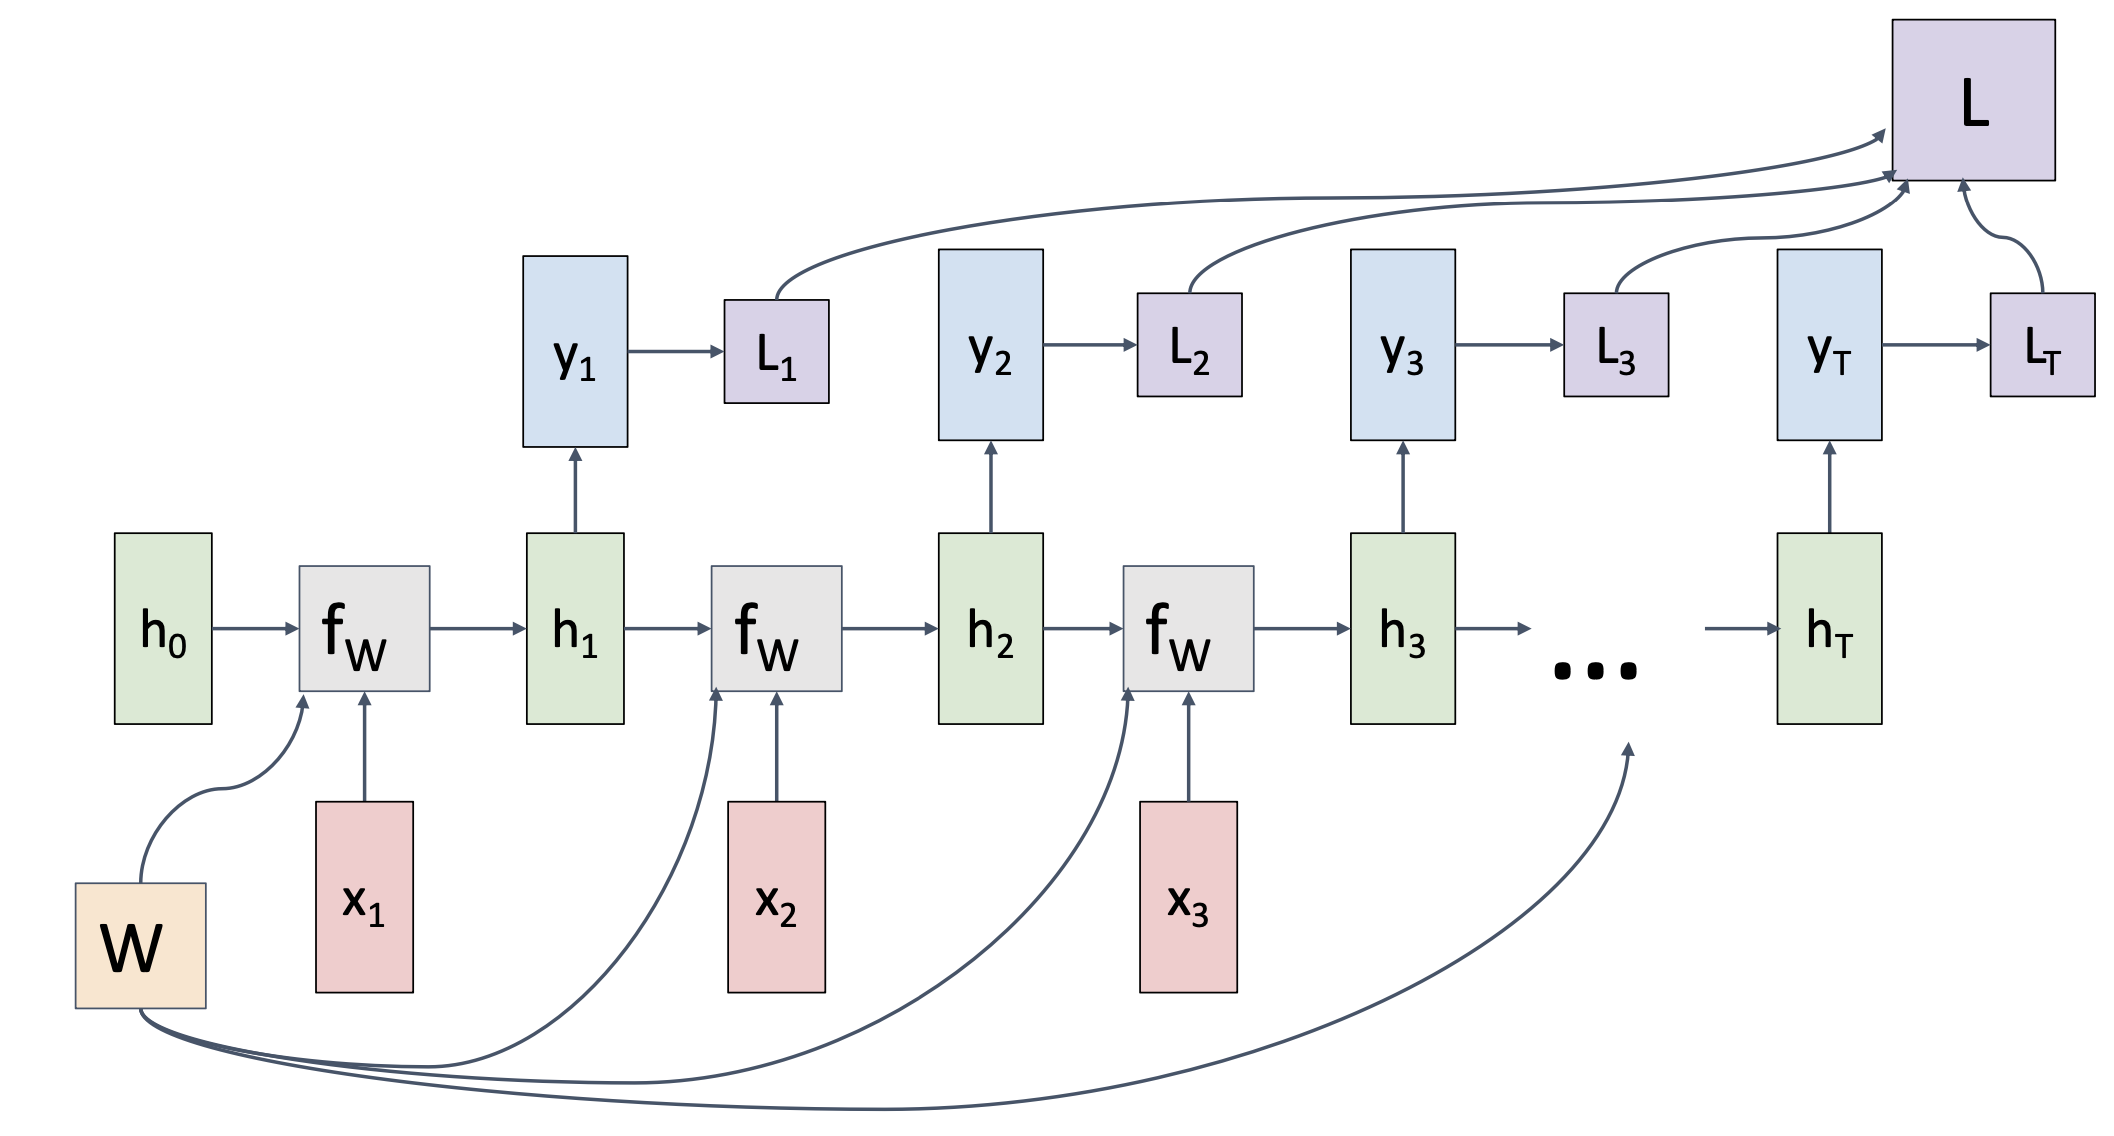
\includegraphics[width=.7\textwidth]{rnn/graph-loss.png}
    \caption{Loss of the unfolded graph.}
\end{figure}
Each output $y_t$ produced can be fed into some loss, for instance by comparing it to some gound truth label. The individual losses $\L_t$ can then be summed into a total loss $\L$, from which the backpropagation will start. Therefore, if we want to compute the gradient $\frac{\partial\L}{\partial W}$, the gradient flow will start in $\L$, separate itself into the different temporal steps $\L_t$, and then combine itself back to $W$ since the parameter is the same at each time step. This is called \emph{backpropagation through time}, as the forward pass is done by generating outputs at increasing time steps, while the backward pass is done starting from the most recently generated outputs.

\subsubsection{Many-to-one, one-to-many, many-to-many}
The previous examples involve a mechanism in which an output $y_t$ is produced for each input $x_t$. In the case of other types of models (many-to-one, one-to-many, mnay-to-many), we might produce no output for certain inputs, or outputs without inputs.

\paragraph*{Many-to-one}
In the many-to-one situation, we usually decide to produce an output only for the final input. The decision is therefore made based only on the final hidden state of the layer, $h_T$; the intuition behind this is that $h_T$ depends on all the previous hidden states $h_t$, and is therefore able to store the information used for the final decision.
\begin{figure}[H]
    \centering
    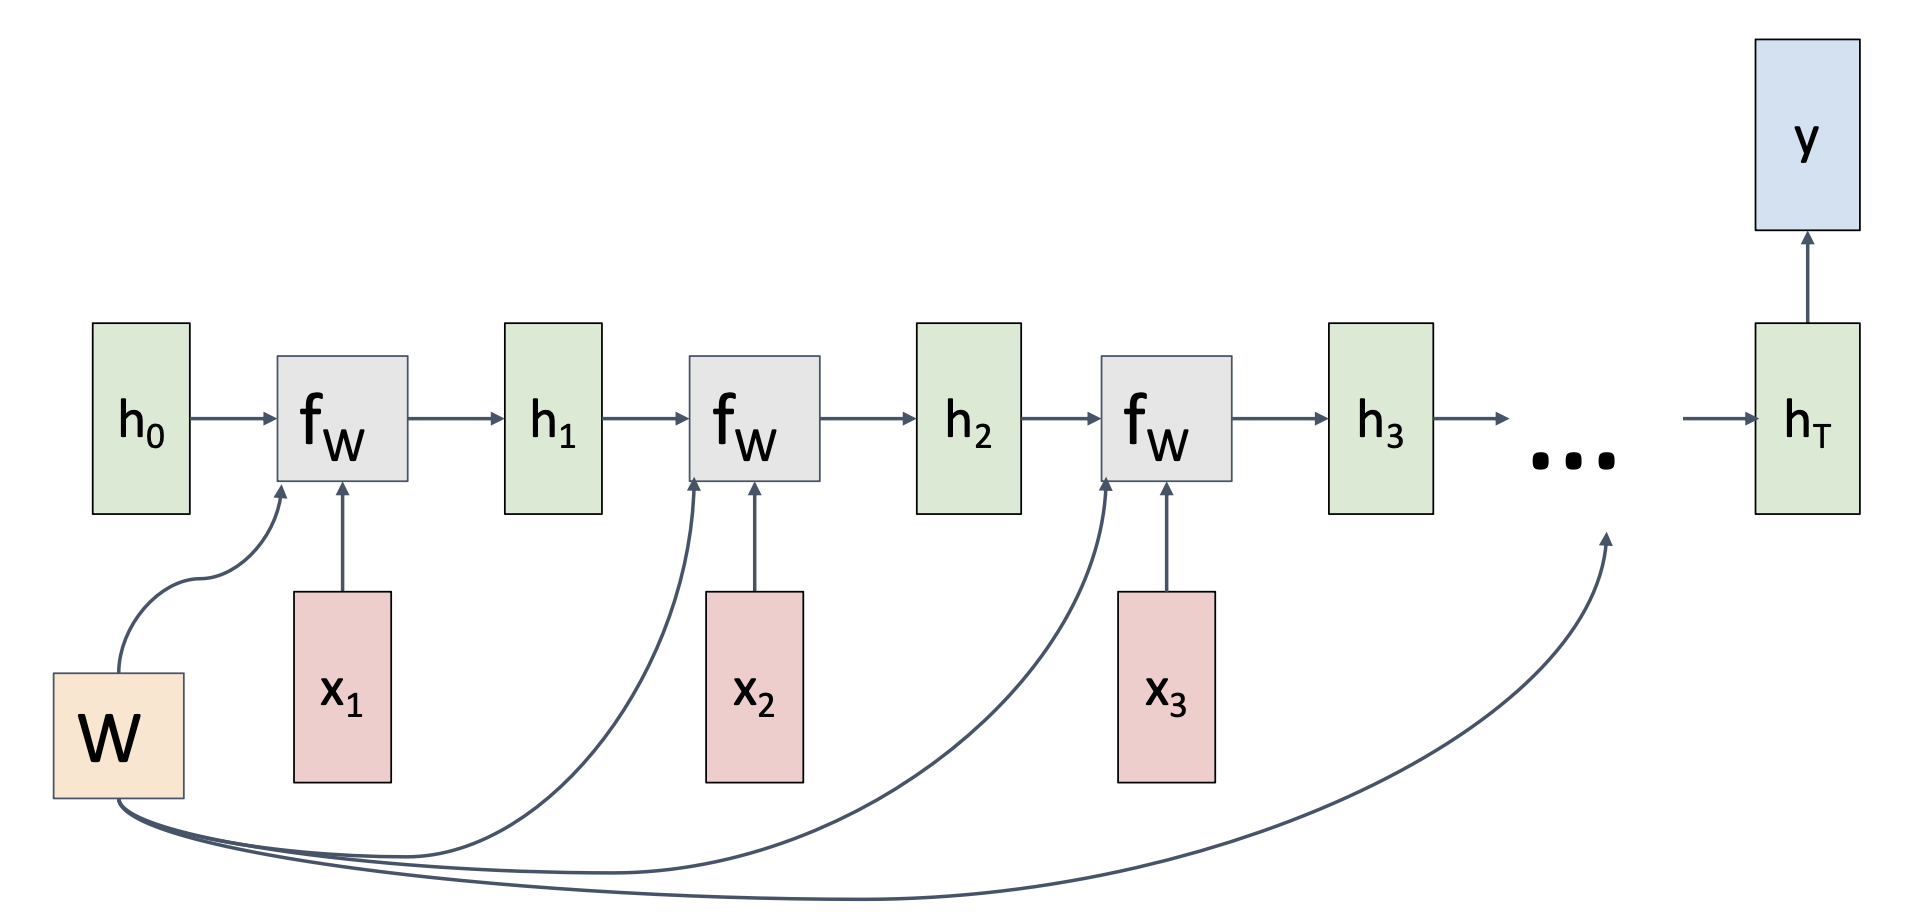
\includegraphics[width=.7\textwidth]{rnn/rnn-many-to-one.png}
    \caption{Many-to-one situation.}
\end{figure}

\paragraph*{One-to-many}
In the one-to-many situation, we typically feed the function with the input only once. After that, the model will keep producing outputs depending solely on the previous hiddens state. This generation process usually stops when a certain output is produced, corresponding to some end-of-file token.
\begin{figure}[H]
    \centering
    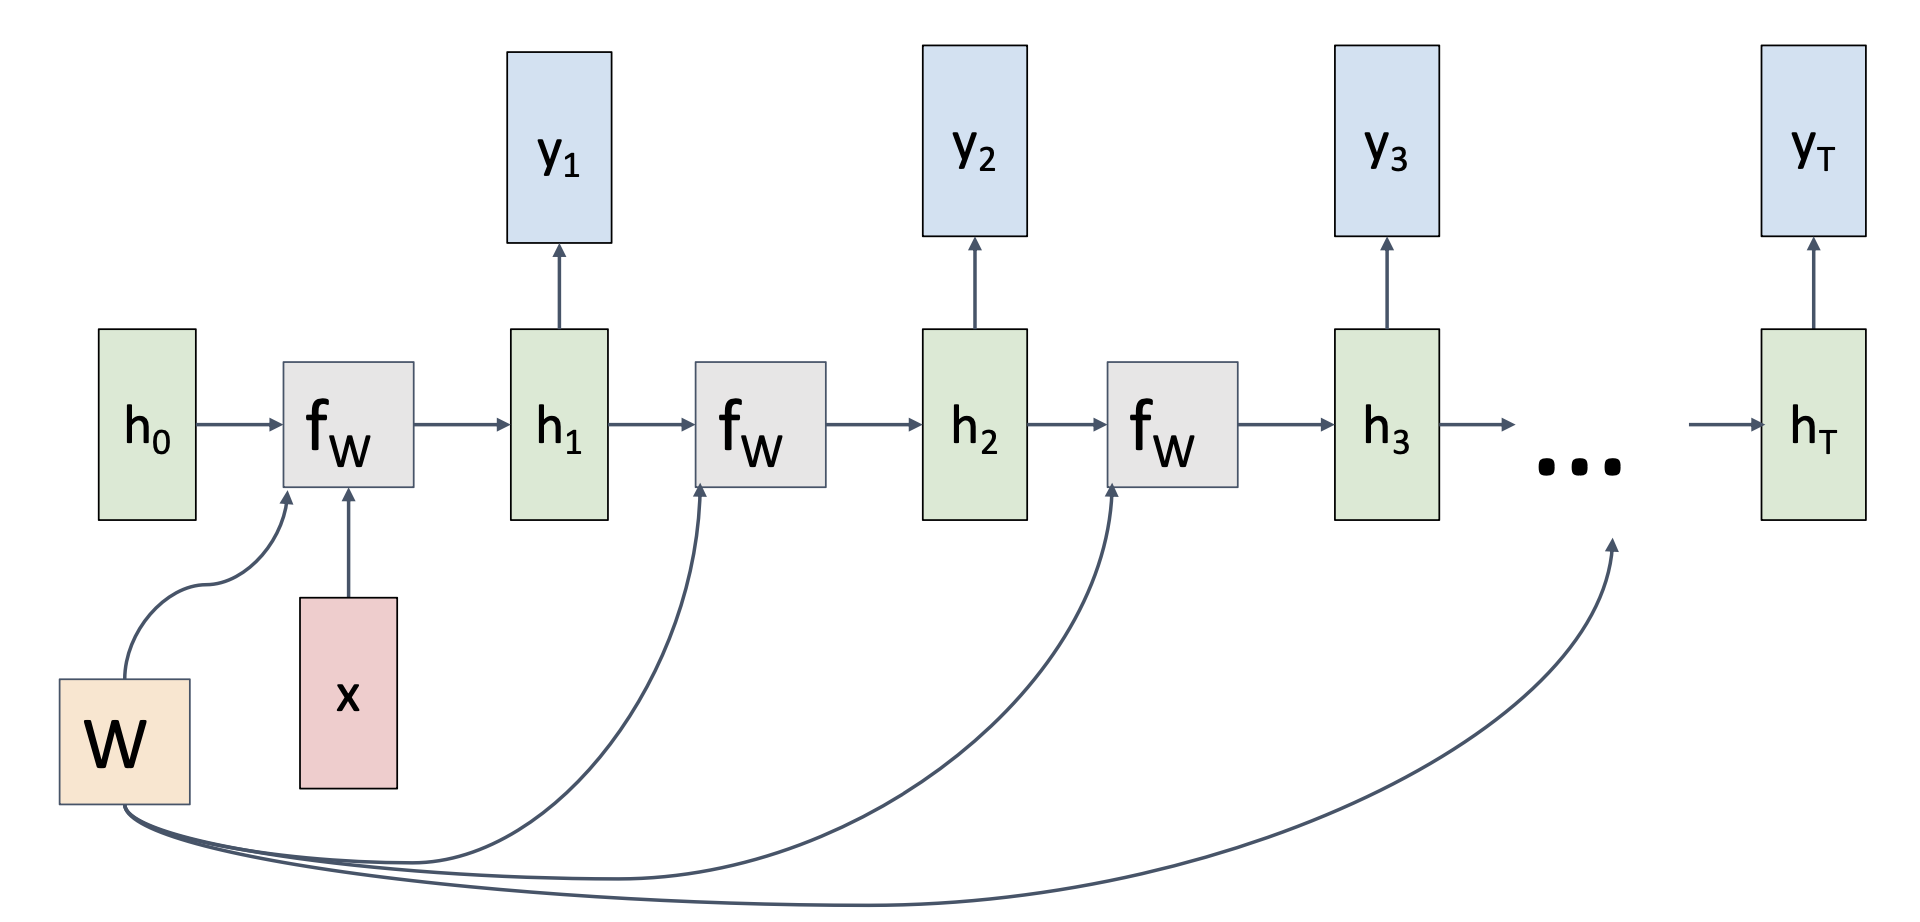
\includegraphics[width=.7\textwidth]{rnn/rnn-one-to-many.png}
    \caption{One-to-many situation.}
\end{figure}

\paragraph*{Many-to-many}
While many-to-one and one-to-many situations are pretty straighforward, many-to-many requires more work, as it would be tricky to manage to make it work with only one recurrent neural network. For instance, in the case of machine translation, it is difficult to produce a translation before the whole input sentence is finished. It seems to be simpler to first read the original sentence, then generate a translated sentence. Furthermore, there is no guarantee that the best hidden states for input understanding are the same as the best hidden states for output generation. Therefore, the sequence to sequence situation is usually handled with two RNNs: an encoder and a decoder.
\begin{figure}[H]
    \centering
    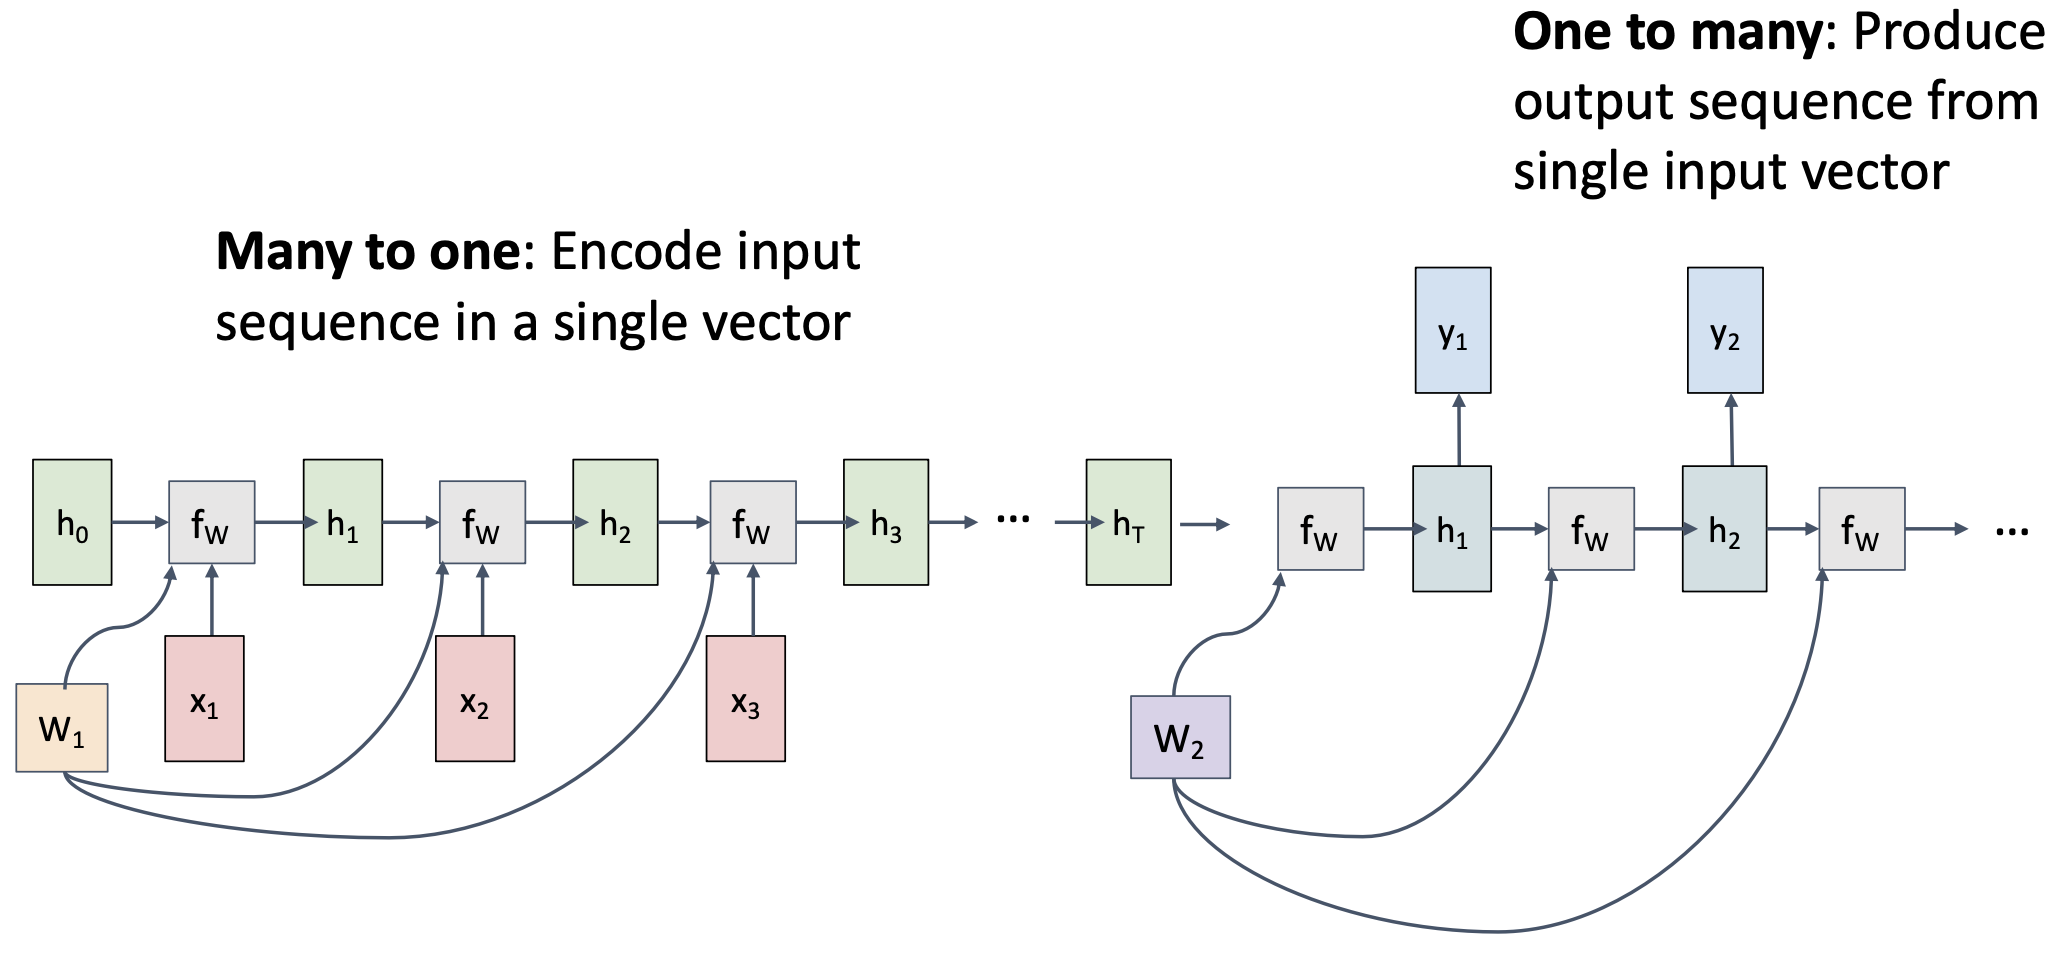
\includegraphics[width=.8\textwidth]{rnn/rnn-many-to-many.png}
    \caption{Encoder and decoder for the many-to-many situation.}
\end{figure}
The encoder will receive the input and summarize it all into the final hidden state of this first many-to-one RNN. This final vector is used by the decoder, a one-to-many RNN, which will use the accumulated context to generate outputs.

\subsubsection{Applications}
Recurrent Neural Networks open the door to many useful and fun applications.

For instance, RNNs can be trained on corpuses of text to generate new sentences following the same style. A nice \texttt{NumPy} implementation of such a vanilla RNN by Andrej Karpathy is available \href{https://gist.github.com/karpathy/d4dee566867f8291f086}{here}\footnote{\href{https://gist.github.com/karpathy/d4dee566867f8291f086}{\nolinkurl{https://gist.github.com/karpathy/d4dee566867f8291f086}}}. When trained on large quantity of text such as Wikipedia, Shakespeare's work or the Linux kernel source code, it can produce new sentences following the style of the text corpus.

\subsection{Gradient Flow in RNNs}
Let's consider the previously introduced vanilla RNN. Its recurrence equation is of the form:
\begin{equation*}
    \begin{aligned}
        h_t &= \tanh\left(W_hh_{t-1}+W_xx_t\right)\\
        &= \tanh\left(W\begin{bmatrix}
            h_{t-1}\\
            x_t
        \end{bmatrix}\right)
    \end{aligned}
\end{equation*}
which corresponds to the following diagram:
\begin{figure}[H]
    \centering
    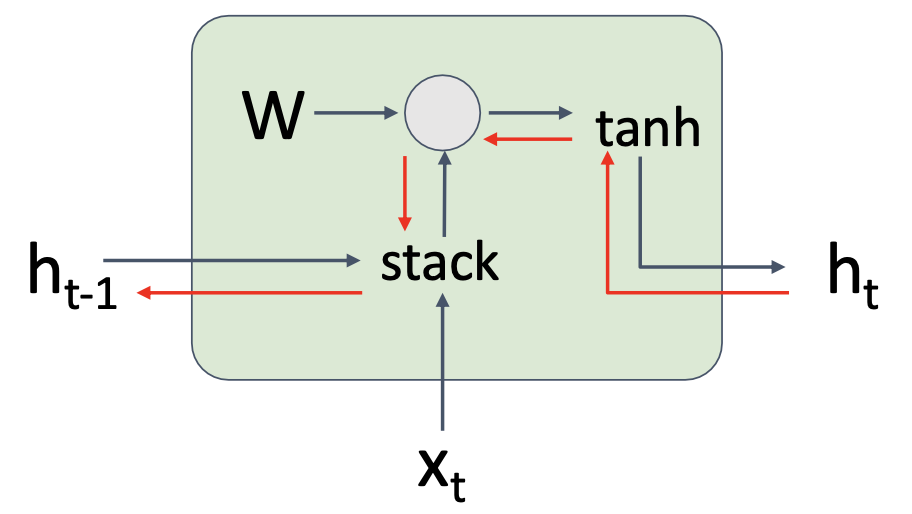
\includegraphics[width=.5\textwidth]{rnn/rnn-backprop.png}
    \caption{Simple computational graph of an RNN cell. Gradient flow is represented in red.}
\end{figure}
This architecture actually causes an issue in the way that the gradient flows throughout the graph. When unrolling the computational graph, we can see that in order to arrive up to $h_0$, the gradient must flow through every previous cell, and will therefore contain as many $W^\tp$ factors as they are time steps.
\begin{figure}[H]
    \centering
    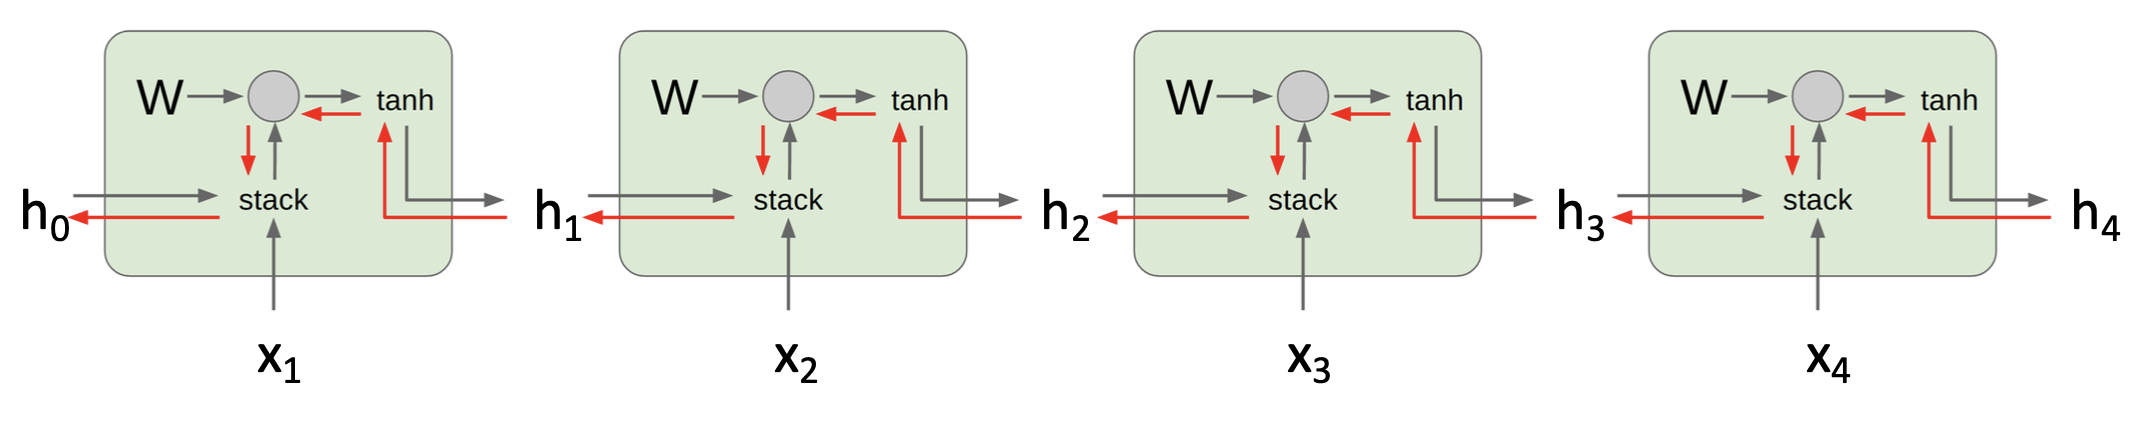
\includegraphics[width=\textwidth]{rnn/rnn-flow-unroll.png}
    \caption{Unrolled computational graph of an RNN. Gradient flow is represented in red.}
\end{figure}
This can cause an issue in one of two possible ways. If the largest eigenvalue of the $W$ matrix is greater than 1, the gradient will explode. If the largest eigenvalue if smaller than 1, the gradient will vanish.

A first solution to avoid the exploding gradient problem is \emph{gradient clipping}. The idea is to scale the gradient if its norm is too big. Formally, we apply the transformation:
\begin{equation*}
    \nabla\L \longleftarrow \begin{cases*}
        \nabla\L \cdot \frac{\theta}{\norm{\nabla\L}} & if $\norm{\nabla\L} > \theta$\\
        \nabla\L & otherwise
    \end{cases*}
\end{equation*}
where $\theta$ is some threshold.

To avoid vanishing gradient, the most widely used solution is to change the recurrent neural network architecture.

\subsection{Long Short-Term Memory (LSTM)}
\subsubsection{Recurrent equation}
The equation defining vanilla recurrent neural network is the following:
\begin{equation}
    h_t = \tanh\left(W\begin{bmatrix}
            h_{t-1}\\
            x_t
        \end{bmatrix}\right)
\end{equation}
The \emph{Long Short-Term Memory} (LSTM) architecture was introduced to solve the vanishing gradient problem. Its recurring equation goes as follows:
\begin{equation*}
    \tag{LSTM}
    \begin{aligned}
        \begin{bmatrix}
            i\\
            f\\
            o\\
            g
        \end{bmatrix}
        &= \begin{bmatrix}
            \sigma\\
            \sigma\\
            \sigma\\
            \tanh
        \end{bmatrix} W \begin{bmatrix}
            h_{t-1}\\
            x_t
        \end{bmatrix} \\
        c_t &= f \odot c_{t-1} + i\odot g\\
        h_t &= o \odot \tanh(c_t)
    \end{aligned}
\end{equation*}
where $\odot$ denotes the Hadamard (component-wise) product.

Instead of keeping only one vector at each time step, two are used: the cell state $c_t$ and the hidden state $h_t$. On top of this, four gates values, $i,f,o$ and $g$ are computed at each time step, which will be used to compute $c_t$ and $h_t$. Each gate can somehow be intuitively interpreted:
\begin{itemize}
    \item \textbf{Input gate} $i$ specifies whether to write in the cell
    \item \textbf{Forget gate} $f$ specifies whether to erase the cell from its previous content
    \item \textbf{Output gate} $o$ specifies how much should the cell be revealed to the hidden state
    \item \textbf{Cell input gate} $g$ specifies what to write in the cell
\end{itemize}
Note that the $g$ gate is the only one to go through a $\tanh$ linearity. The $i,f$ and $o$ gates have coefficients in $[0,1]$, which fits the opened/closed gate interpretation, while $g$ has coefficients in $[-1,1]$, which is the range of values of $c_t$.

The new cell value is a combinaison of its previous value $c_{t-1}$ and the cell input gate $g$: the proportion of both values are controlled by the forget gate $f$ and the input gate $i$. The new $c_t$ value being computed, it is sent to the classical hidden state $h_t$; the output gate $o$ controls what coefficients are being sent.

\subsubsection{Gradient flow}
While it might seem very complex, LSTM improves the gradient flow throughout the cell. An important behavior is that the gradient propagation from $c_t$ to $c_{t-1}$ only passes through an element-wise multiplication by $f$, and no matrix multiplication by $W^\tp$.
\begin{figure}[H]
    \centering
    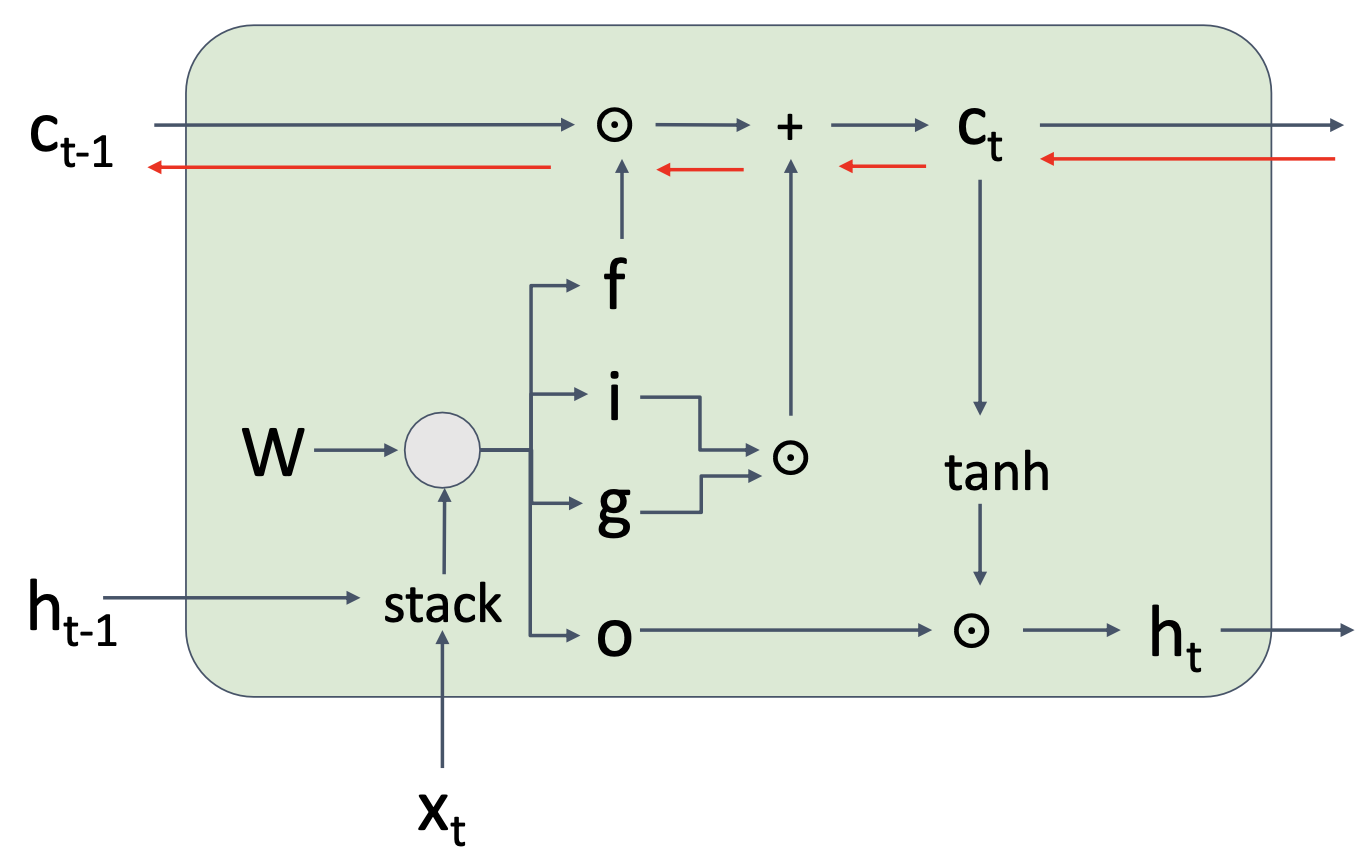
\includegraphics[width=.5\textwidth]{rnn/lstm-flow.png}
    \caption{Gradient flow through an LSTM cell.}
\end{figure}

Therefore, chaining together multiple LSTM cells by unrolling the computational graph does not make the gradient vanish if $f$ is working correctly: it creates an uninterrupted gradient flow from late cell states to early state cells.
\begin{figure}[H]
    \centering
    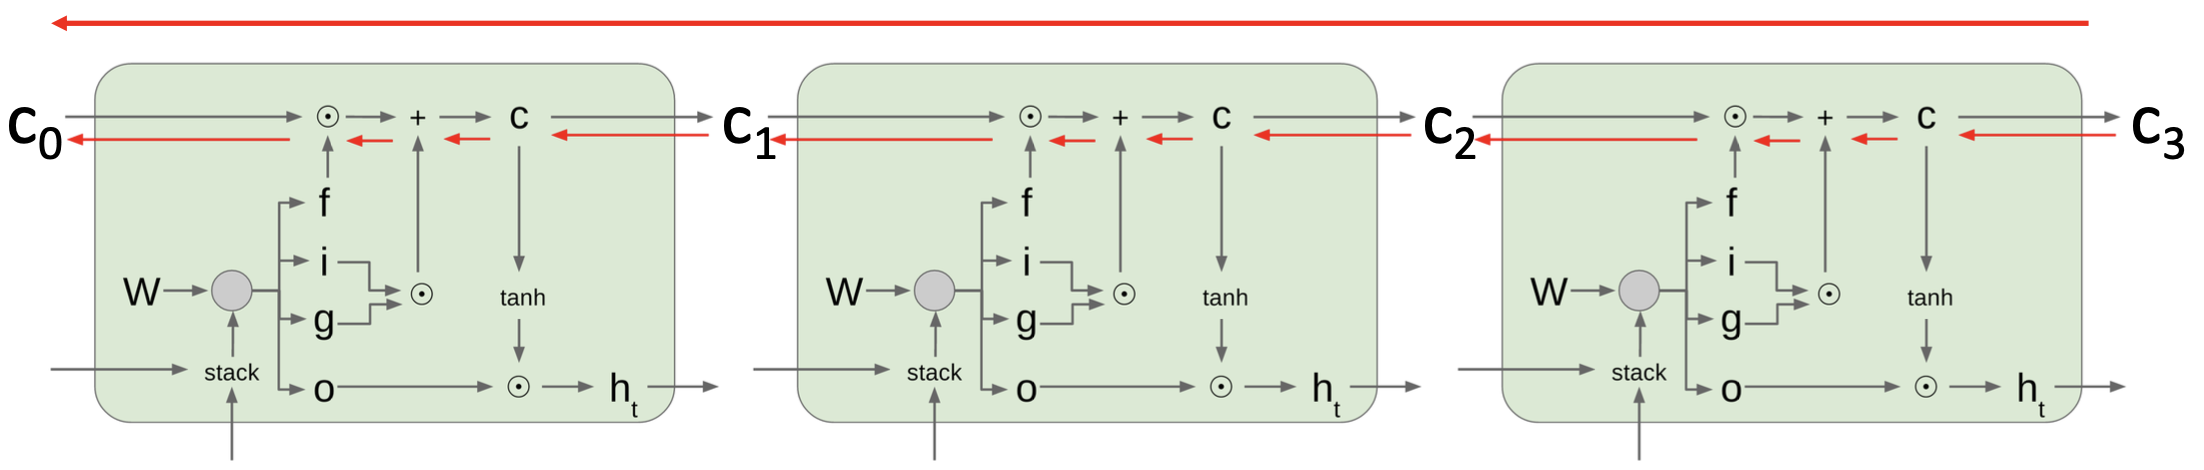
\includegraphics[width=\textwidth]{rnn/lstm-uninterrupted-grad.png}
    \caption{Uninterrupted gradient flow.}
\end{figure}

\subsection{Multilayer Recurrent Neural Networks}
So far, we only considered the use of a recurrent neural network with only one hidden cell. Empirically, neural networks with more layers often perform better, as we saw for MLPs and CNNs. We would like to apply this layering idea to RNNs.

The idea of multilayer RNNs is to feed then hidden states produced at each time steps into a second RNN, with different weight matrices.
\begin{figure}[H]
    \centering
    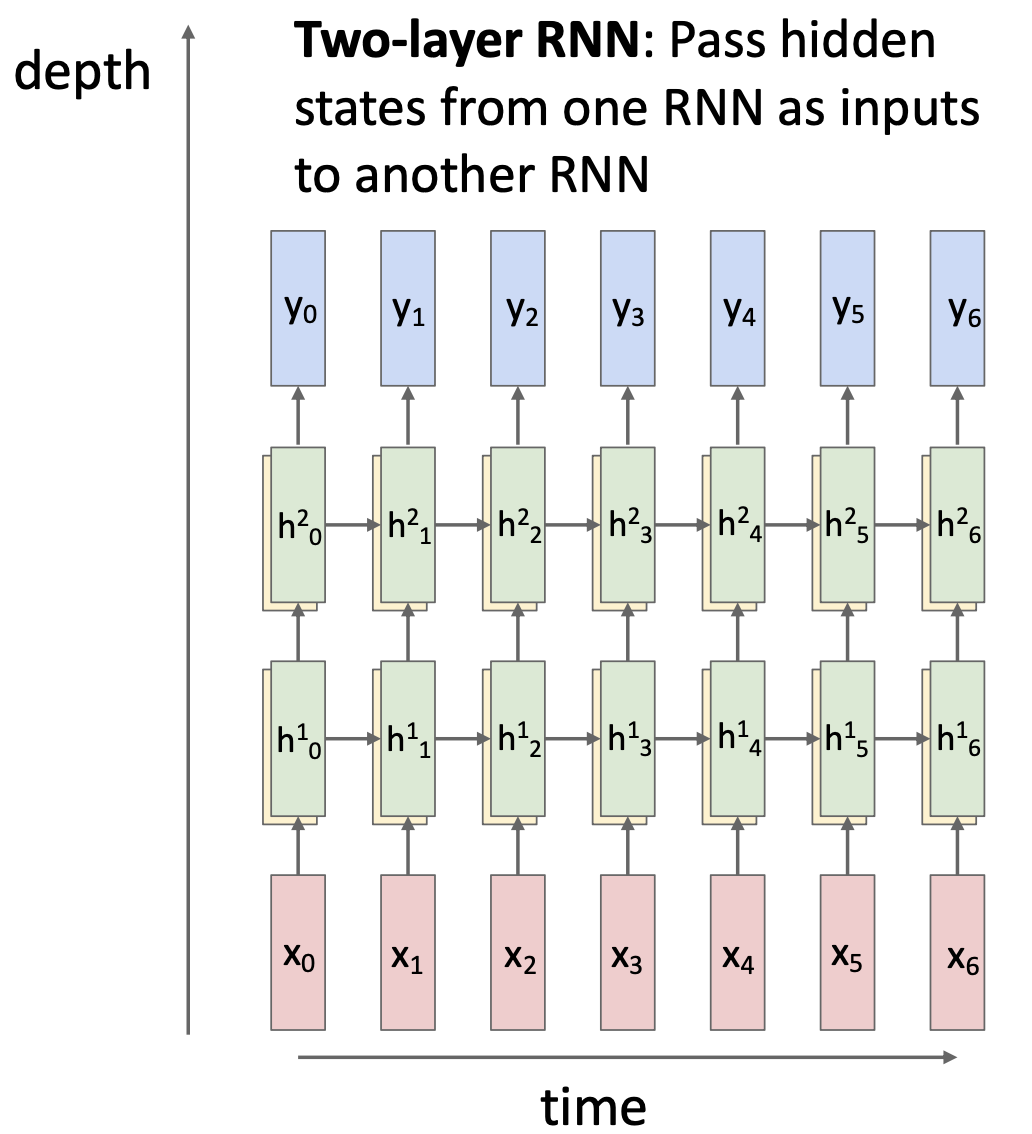
\includegraphics[width=.5\textwidth]{rnn/two-layer-rnn.png}
    \caption{A two-layer RNN.}
\end{figure}
This process can be iterated to create deep recurrent neural networks, by adding two, three, ore more RNNs on top of each other. Note that while it is very common for CNNs to have very deep networks, RNNs are often used in practice with no more than three or four layers.

\subsection*{RNN: Summary}
RNNs give us a lot of flexibility in architecture design by allowing one/many to one/many models. Vanilla RNNs are simple but don't work so well, because of exploding and vanishing gradients. LSTM is the most commonly used alternative to vanilla RNNs, used to solve the vanishing gradient problem.

%But RNNs cells can also be combined to form multi-layer architectures. In a multi-layer RNN, the input is fed into a first hidden state, which is then used as the input for a second hidden state (another layer), which is eventually passed into a feed-forward layer to produce an output.
\section{Attention and Transformers}
\subsection{Sequence-to-sequence with RNNs and attention}
\subsubsection{Encoder-decoder RNNs and limitations}
Originally, the transformer architecture was proposed for machine translation, and was later extended to other deep learning domains. To introduce the attention mechanism, let's consider a machine translation setup; we will start by building up on top of the RNN architecture introduced in the previous chapter.

We are given a sentence in English and want to translate it in French. To do so, we use two RNNs, an encoder which will handling the input tokens, and a decoder which will generate the output sentence.
\begin{figure}[H]
    \centering
    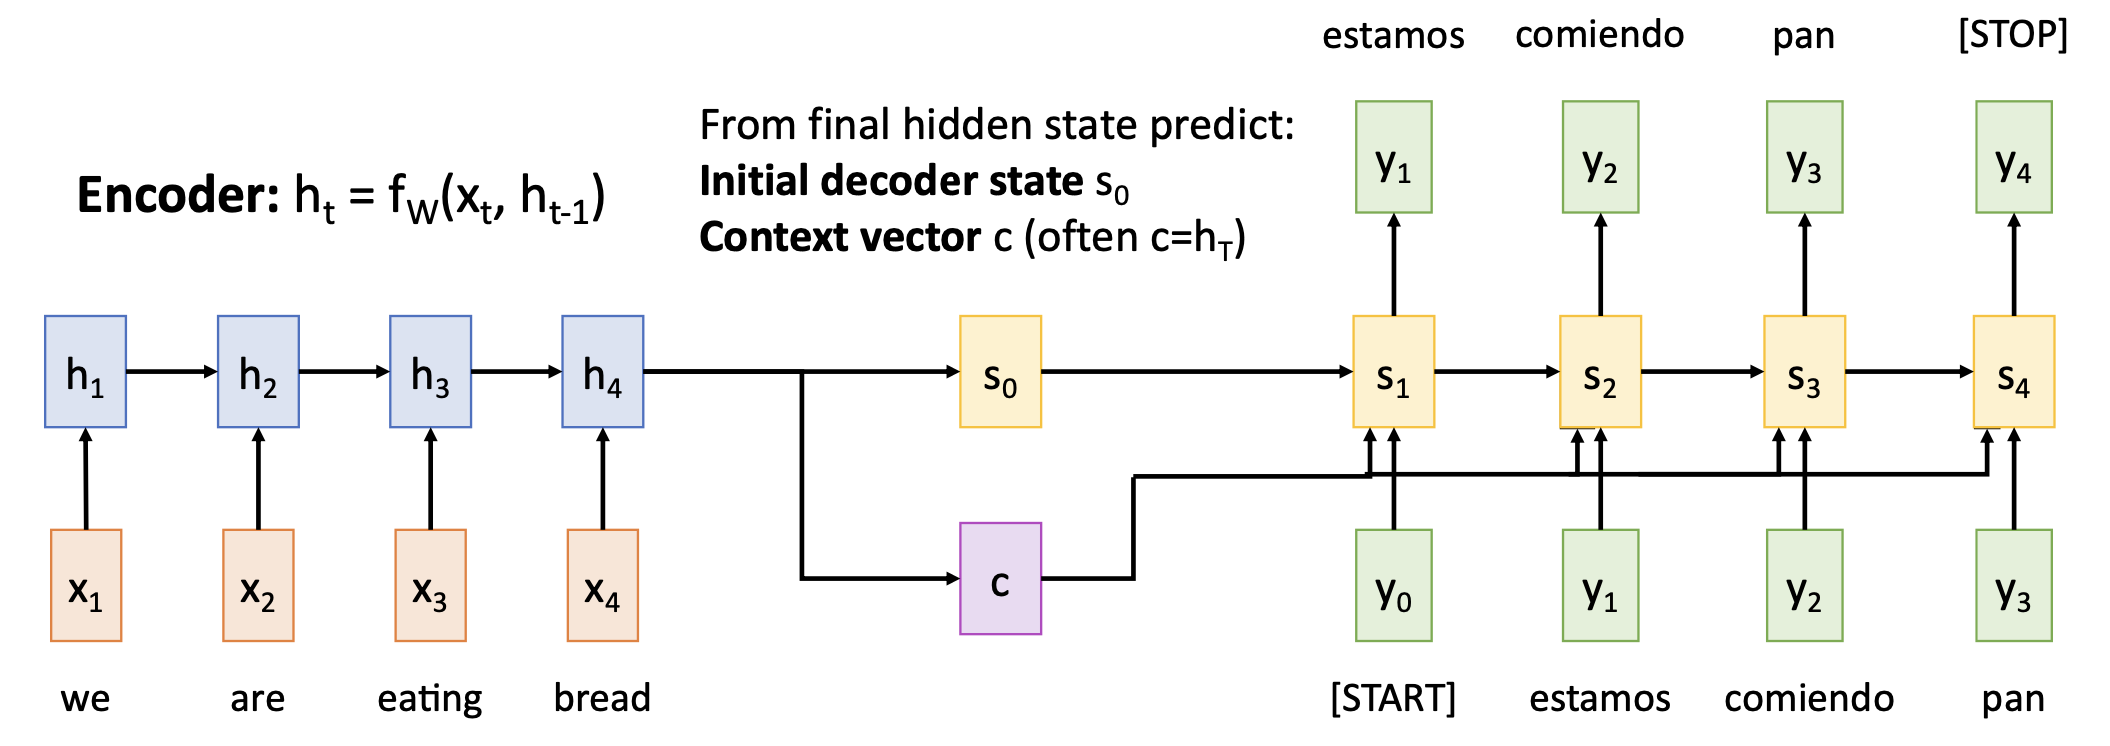
\includegraphics[width=\textwidth]{images/seq-to-seq.png}
    \caption{Sequence-to-sequence using an RNN.}
\end{figure}
After the processing of the original sentence, the encoder will summarize the entire context of that input sentence using two vectors: the initial decoder state $s_0$, and the context vector $c$. In practice, $s_0$ is often obtained by feeding $h_T$ through a feed-forward neural network, and $c$ is often set to $h_T$ directly.

The decoder will receive a start token $y_0$ as its first input, as well as the context vector $c$; it will then generate the first output token $y_1$, which will be used as the second input. Note that the context $c$ is fed to the decoder at each step of the generation, on top of the last generated token $y_t$. Formally, its recurring equation is of the form:
\begin{equation*}
    s_t = g_{W'}(y_{t-1}, s_{t-1}, c)
\end{equation*}

While this architecture is fairly reasonable, its bottleneck is that the entire context of the sentence must be summarized in the fixed-size context vector $c$. If the text to translate is too long (think of an entire book for instance), the model will not be able to fit all the context details in $c$. The idea to solve this issue is to compute a new context vector at each step of the decoder, and to allow the decoder to reconstruct the context vector by using different vectors focusing on different parts of the original sentence. This mechanism is called \emph{attention}.

\subsubsection{The attention mechanism}
We will keep the general encoder-decoder structure, but instead change the way that the context is passed from the encoder to the decoder. We will use an MLP called $f_{\textnormal{att}}$, which will compute scalar alignment scores:
\begin{equation*}
    e_{t,i} = f_{\textnormal{att}}(s_{t-1}, h_i)
\end{equation*}
Intuitively, the alignment score $e_{t,i}\in\R$ quantifies how much \emph{attention} should be put in the hidden state of the encoder $h_i$, given the hidden state of the decoder $s_{t-1}$. These scalars will be used to construct a new context vector at each step of the decoder.

\begin{figure}[H]
    \centering
    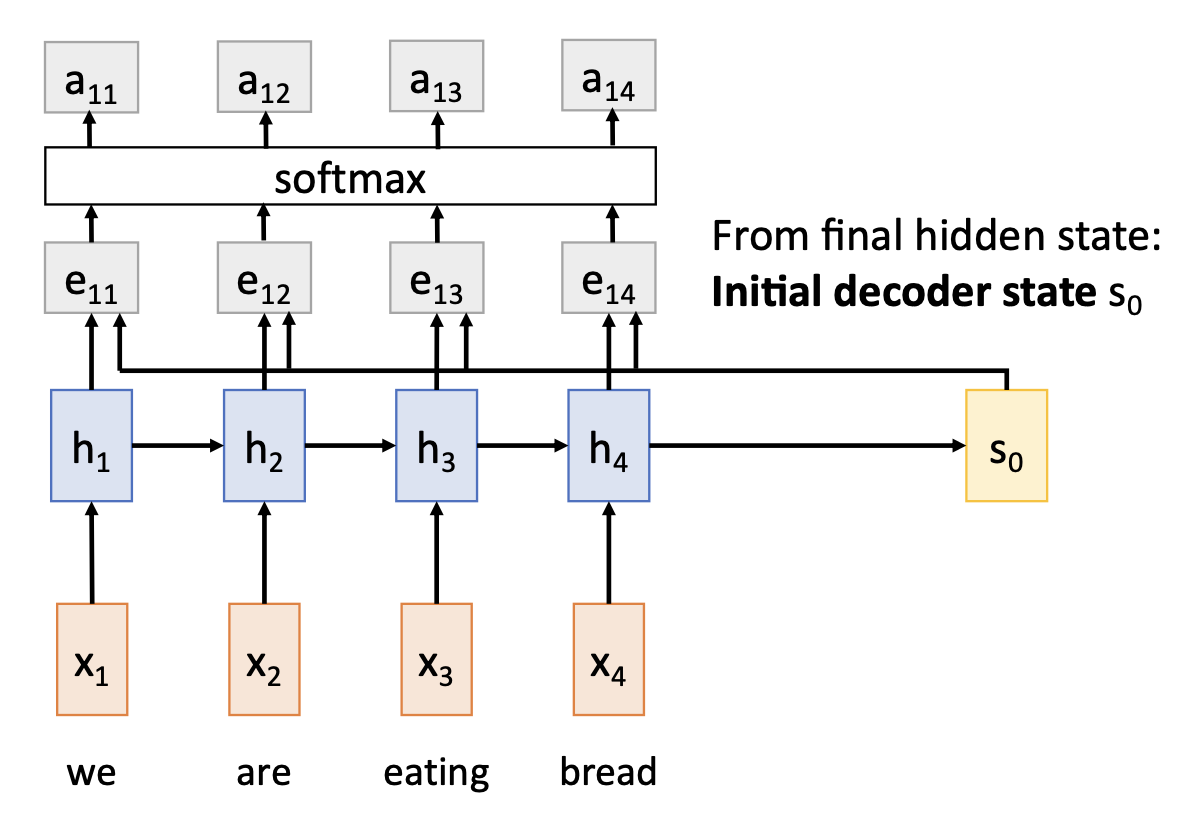
\includegraphics[width=.5\textwidth]{images/attention-scores.png}
    \caption{Applying softmax to alignment scores gives us attention scores.}
\end{figure}

The alignment scores are arbitrary real numbers. Therefore, we apply to them the softmax operations for each decoder state $s_{t-1}$, giving us \emph{attention weights} $(a_{t,i})$ satisfying:
\begin{equation*}
    \sum_i a_{t,i} = 1 
\end{equation*}
That being done, we can finally compute the context vector for each time step $t$ of the decoder, using a sum of the hidden states $(h_i)$ weighted by the attention scores $(a_{t,i})$:
\begin{equation*}
    c_t = \sum_i a_{t,i}\cdot h_i
\end{equation*}
This gives us the context vector $c_t$ which will be used for the generation of $y_t$ by the decoder. Note that this is all differentiable and allows us to backpropagate through the parameters of $f_{\textnormal{att}}$; in particular, we do not need to supervise the attention weights.
\begin{figure}[H]
    \centering
    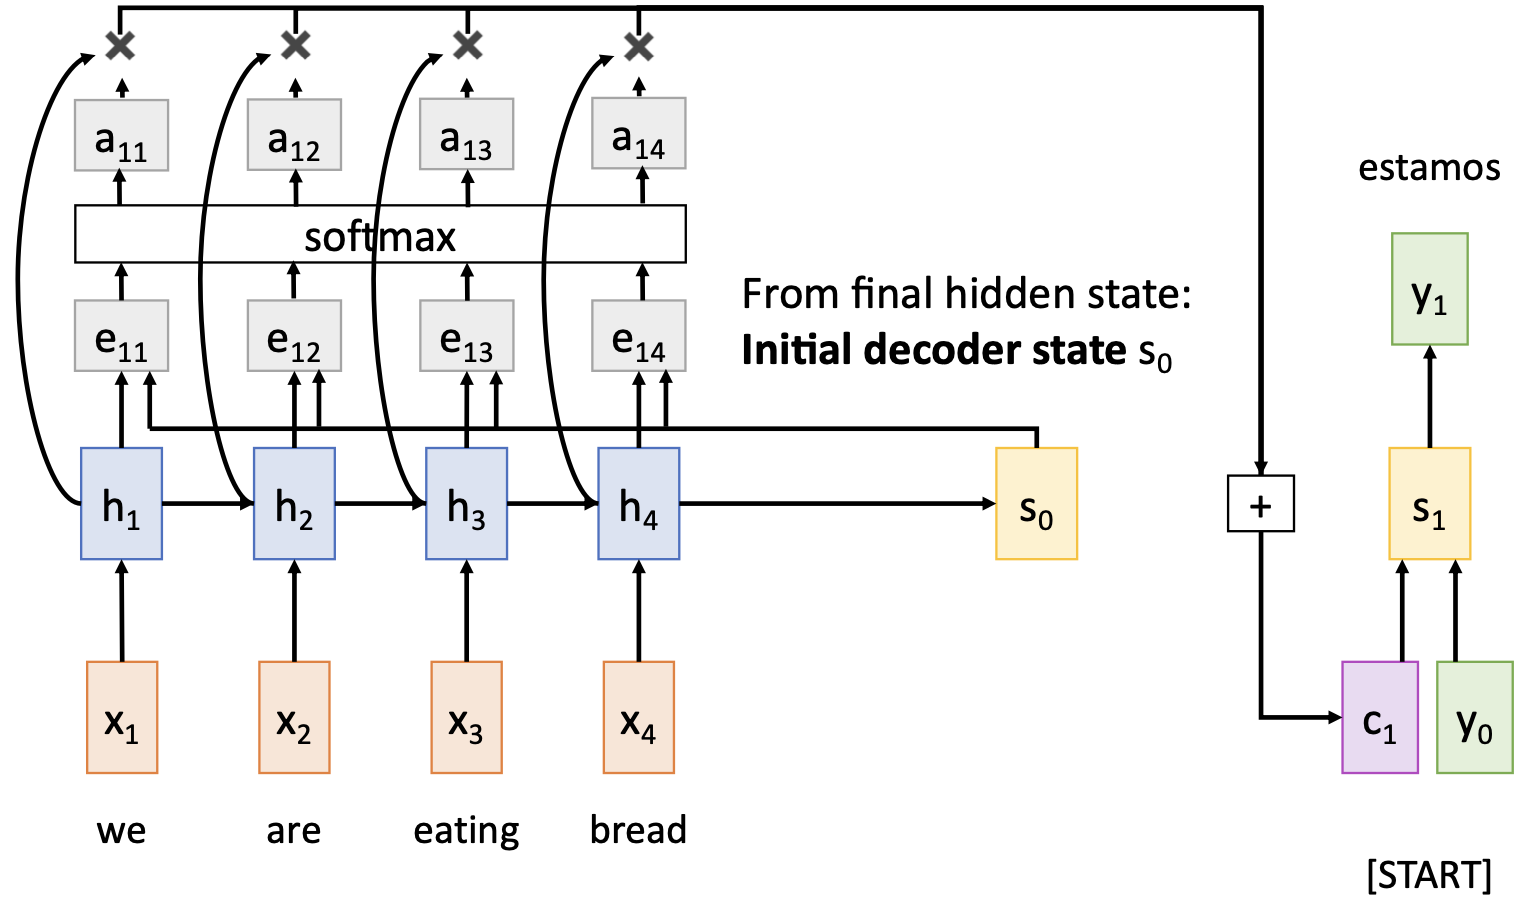
\includegraphics[width=.65\textwidth]{images/attention-context.png}
    \caption{Computation of the context vector using attention scores.}
\end{figure}
This process that was applied for the first decoder step $t=1$ can be iterated for every following step: we compute the alignment scores using the new hidden state $s_1$, then the attention scores, giving us the context vector $c_t$, which is fed into the decoder alongside $y_{t-1}$.
\begin{figure}[H]
    \centering
    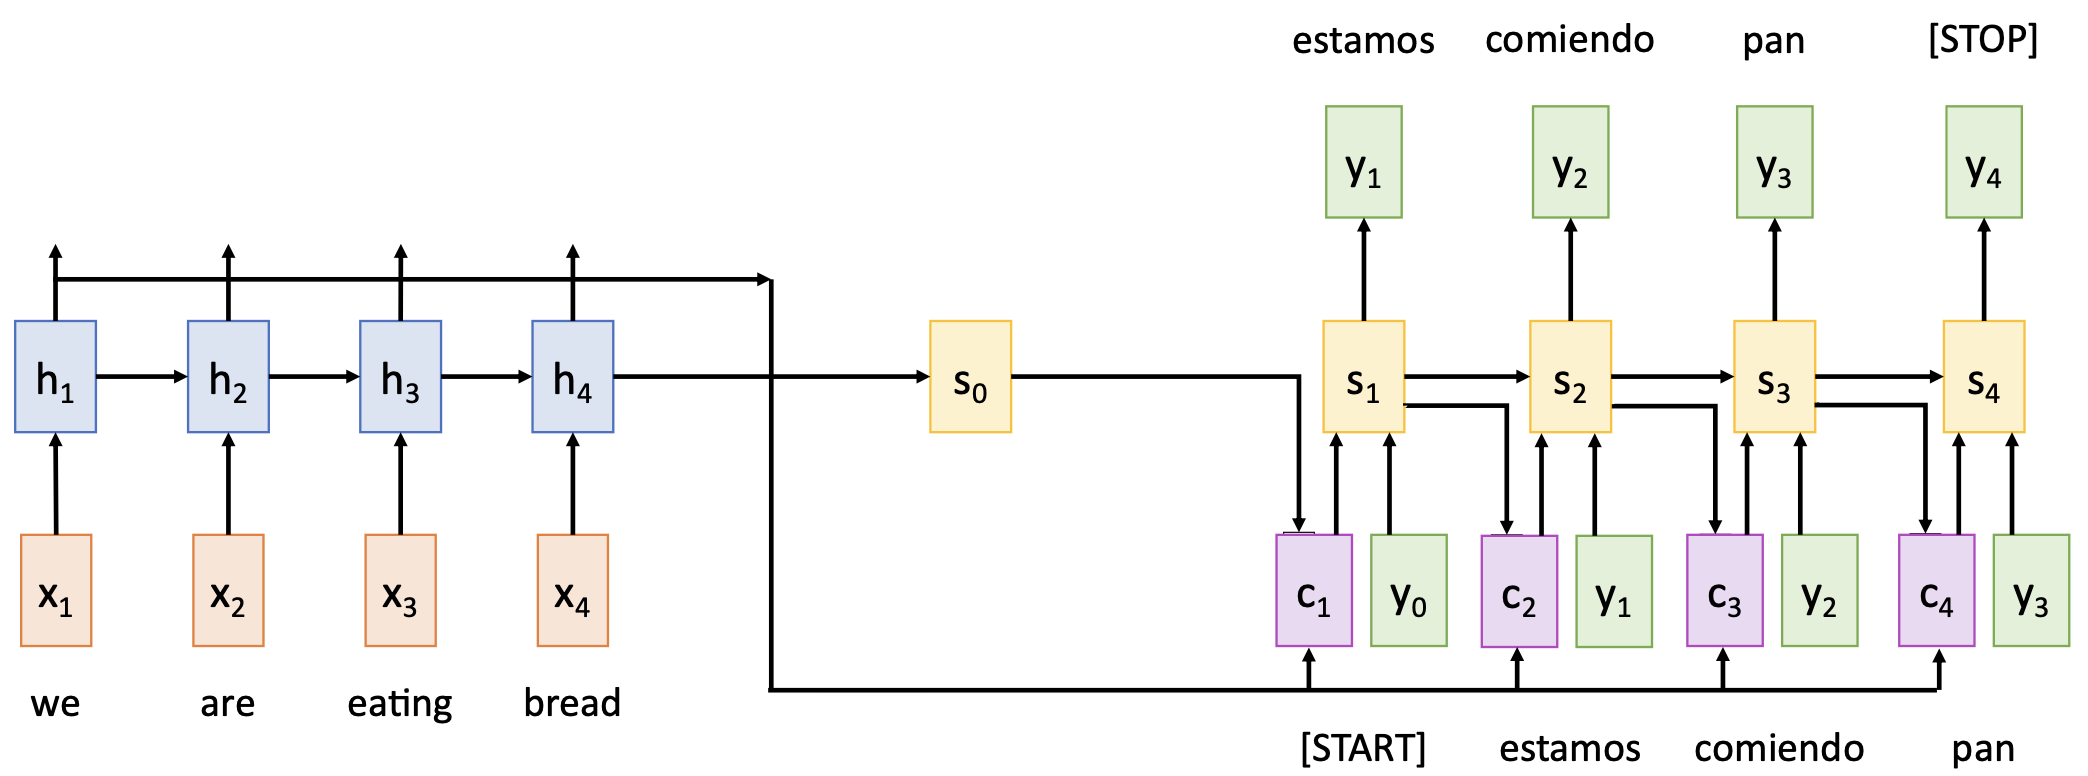
\includegraphics[width=.9\textwidth]{images/attention-unrolled.png}
    \caption{Unrolling the computational graph with attention.}
\end{figure}
This overcomes the bottleneck problem encountered for unique context vectors: at each step, the decoder is able to choose the relevant hidden states of the encoder, which selects only relevant information. When working with very long sequences, the model will be able to shift its attention around and focus on important parts of the inputs.

\subsection{Visualizing and interpreting attention weights}
\begin{wrapfigure}[14]{r}{.45\textwidth}
    \captionsetup{justification=raggedleft}
    \centering
    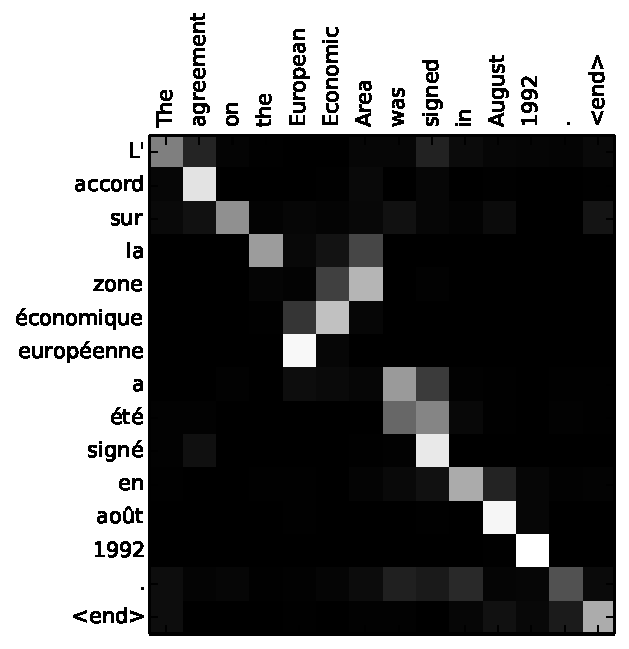
\includegraphics[width=.45\textwidth]{images/attention-visualization.pdf}
    \caption{Visualization of attention weights for English-to-French translation.\protect\footnotemark}
\end{wrapfigure}
\footnotetext{Image taken from Bahdanau et al, \say{Neural machine translation by jointly learning to align and translate}, ICLR 2015}
The attention weights can be used to gain interpretability of the model: we can see for each output word which original words it was the most focused on.  

Diagonal attention (the first four words and the last 5 words) means that words correspond in order between French and English. High coefficients outside the diagonal (for instance, \say{European}/\say{européenne}) show words out of order between the two sentences. Finally, some lines and columns have more than one non-zero coefficient, such as the \say{was} or \say{say} columns: these show that the verb conjugation requires more than one word of context to be translated.

\newpage
\subsection{Image captioning with RNNs and Attention}
It is important to notice that the decoder does not use the fact that the hidden states $(h_i)_i$ form an ordered sequence, but only considers them as an unordered set $\set{h_i}{i\in I}$. This means that we can use the same architecture given any set of input hidden vectors $\set{h_i}{i\in I}$, especially for other types of data that do not form sequences.

Consider a deep convolutional neural network, without fully-connected layers at the end. The ouput of this CNN can be interpreted as a grid of feature vectors of the image. We see these feature vectors just like a sequence of hidden states of an encoder RNN: we can therefore apply the attention mechanism to them. We consider a simple model $f_{\textnormal{acc}}$ that we use to compute the alignment scores of each feature in the grid:
\begin{equation*}
    e_{t,i,j} = f_{\textnormal{att}}(s_{t-1}, h_{i,j})
\end{equation*}
We then pass each grid of alignment scores into the softmax operator, giving us a normalized probability distribution, the grid of attention weights $(a_{t,i,j})$. Once again, the context of the image can be summarized with respect to the attention weights by computing a context vector $c_t$:
\begin{equation*}
    c_t = \sum_{i,j} a_{t,i,j} \cdot h_{i,j}
\end{equation*} 
Feeding the context vector $c_1$ alongside the start token $y_0$ into the decoder RNN starting with hidden state $s_0$ can be used to generate a caption corresponding to the image.
\begin{figure}[H]
    \centering
    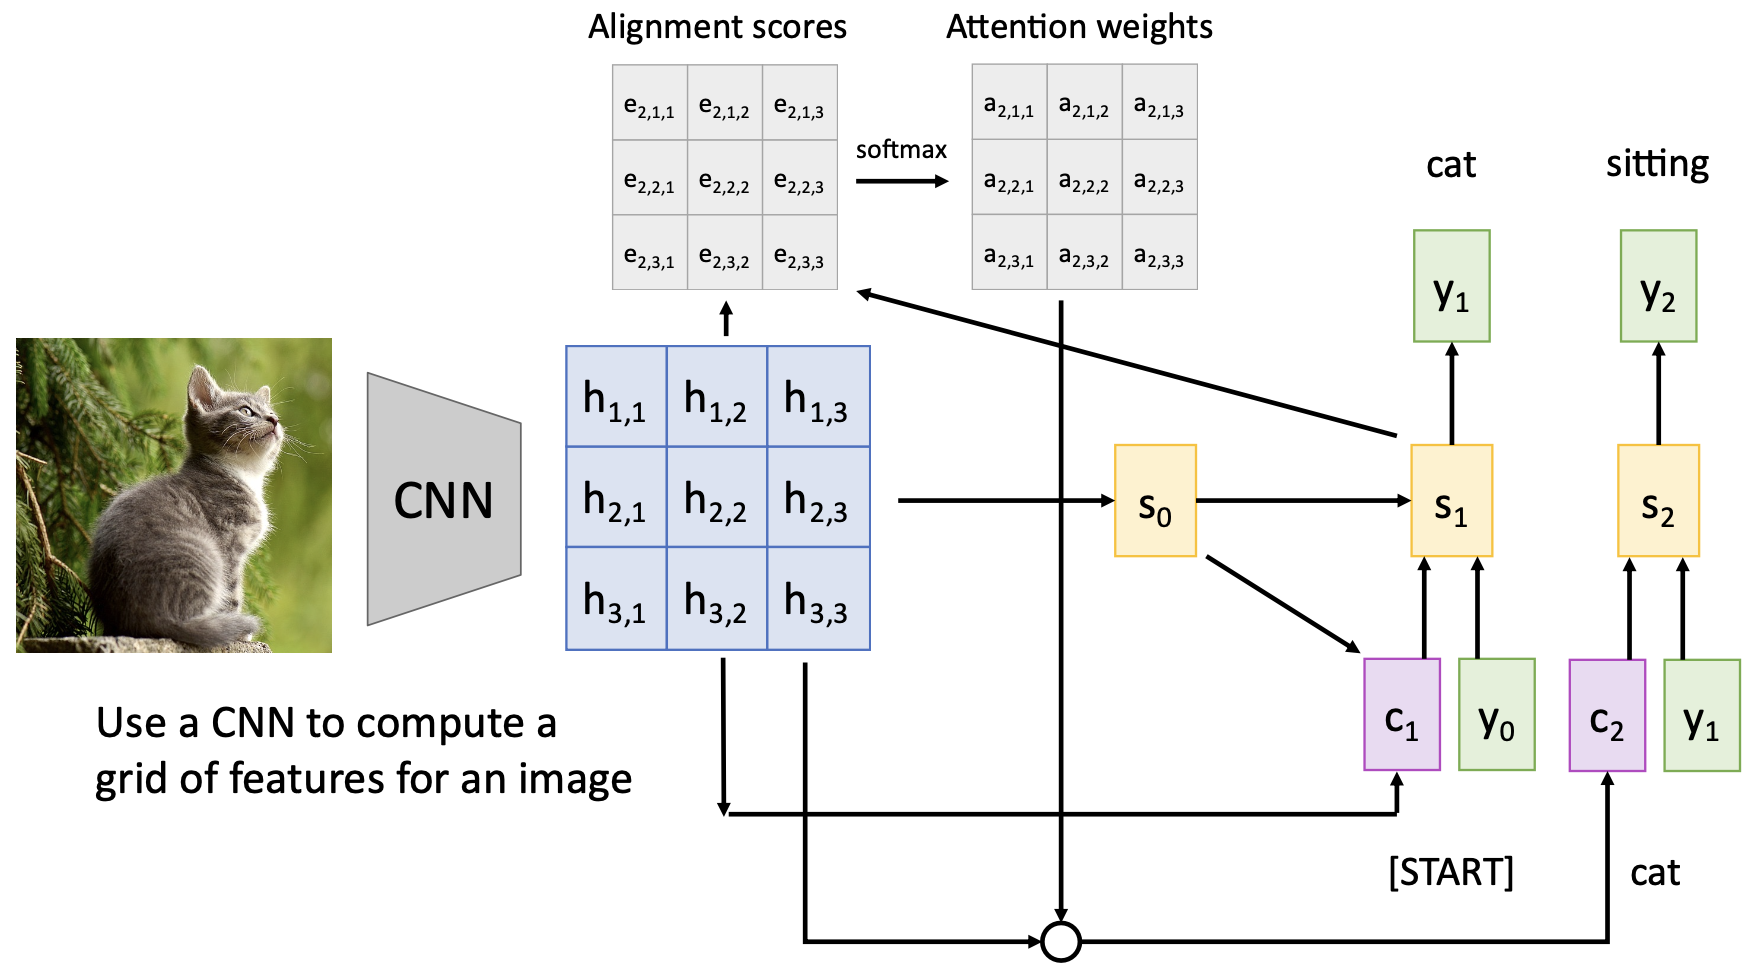
\includegraphics[width=.9\textwidth]{images/attention-cnn.png}
    \caption{Applying attention to a grid of features for image captioning.}
\end{figure}

\begin{figure}[H]
    \centering
    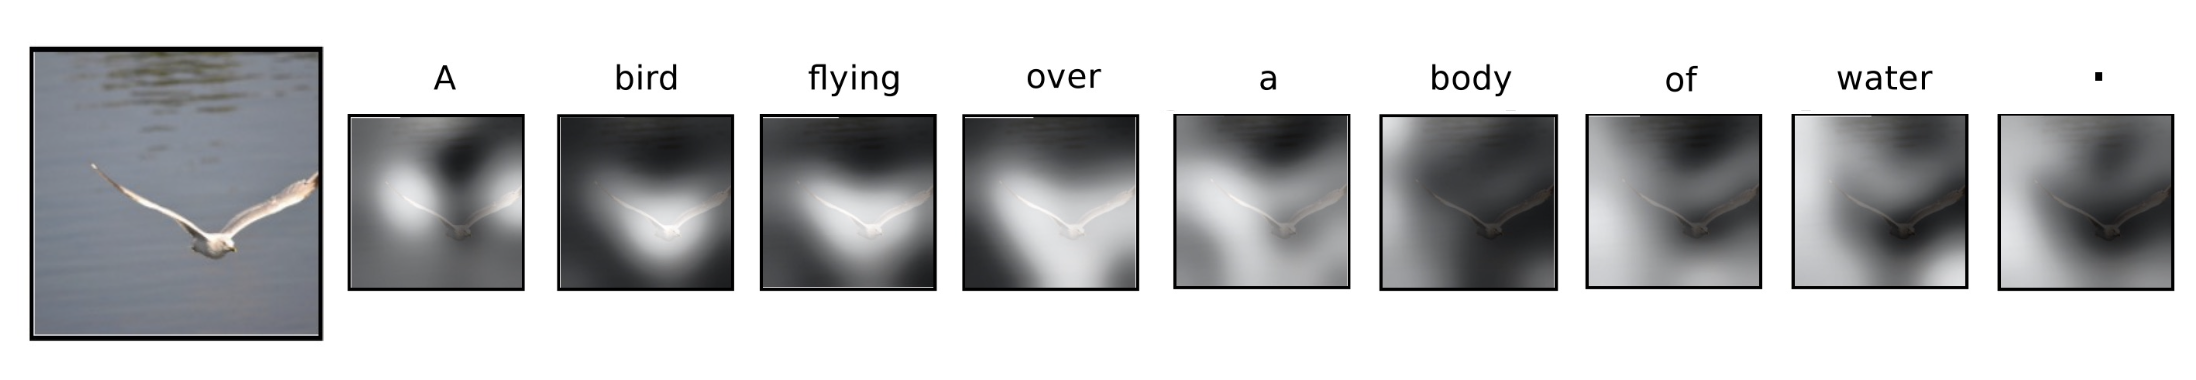
\includegraphics[width=\textwidth]{images/attention-bird.png}
    \caption{Visualizing attention over time during captioning.\protect\footnotemark}
\end{figure}
\footnotetext{Image taken from Xu et al, \say{Show, Attend, and Tell: Neural Image Caption Generation with Visual Attention}, ICML 2015}

\newpage
\section{Regularity and Robustness}
\subsection{Stability during training}

\subsection{Generalization beyond the training samples}

\subsection{Robustness and adversarial attacks}
\section{Deep Reinforcement Learning}
\subsection{What is Reinforcement Learning?}
Machine learning problems can be distinguished in three major paradigms. Given a set of inputs and corresponding outputs, \emph{supervised learning} tries to learn the function mapping inputs to outputs. \emph{Unsupervised learning} studies the structure of data, without being given labels. The third paradigm is called \emph{reinforcement learning}: such problems aim at optimizing the actions of an agent in an environment to maximize its reward.

Formally, we control an agent that can observe at each time step $t$ the \emph{state} of the environment, $S_t$. It can use this state to choose an action $A_t$, to which the environment will reply with a reward $R_t$, and a new state $S_{t+1}$.
\begin{equation*}
    S_t\longrightarrow A_t\longrightarrow R_t \Longrightarrow S_{t+1}\longrightarrow A_{t+1} \longrightarrow \dots
\end{equation*}
This is called one \emph{episode} of learning.

\subsection{Markov Decision Process}
\subsubsection{Formalisation}
The \emph{Markov Decision Process} (MDP) is a mathematical formulation of the Reinforcement Learning process. It makes the assumption of the \emph{Markov property}: the current state completely caracterizes the state of the world.

\begin{definition}[Markov Decision Process]
    A Markov Decision Process is a 5-tuple $(\S, \A, \Rc, \P, \gamma)$ where:
    \begin{itemize}
        \item $\S$ is the set of all states
        \item $\A$ is the set of possible actions
        \item $\Rc:\S\times\A\to\R$ is a function mapping a (state, action) pair to an immediate reward
        \item $\P$ is a probability distribution; for $s,s'\in\S$, $a\in\A$, $\P(S_{t+1}=s'|S_t=s,A_t=a)$ is the probability to transition from state $s$ to state $s'$ after choosing the action $a$.
        \item $\gamma\in[0,1]$ is a \emph{discount factor}, quantifying how much we value rewards coming soon conversely to rewards coming later. $\gamma=1$ values equally all future rewards, while $\gamma=0$ means that we only care about the next reward.
    \end{itemize}

    Initially (at time step $t=0$), an initial state $S_0$ is sampled. Then for any $t\in\iset{0}{T}$\footnote{We might have $T=+\infty$} the following process is iterated:
    \begin{itemize}
        \item The agent chooses an action $A_t$
        \item The environment computes the associated reward $R_t=\Rc(S_t,A_t)$
        \item The environment samples the next step $S_{t+1}\sim\P(\cdot|S_t,A_t)$
        \item The agent receives the reward $R_t$ and the next step $S_{t+1}$
        \item \dots
    \end{itemize}
\end{definition}

\begin{definition}[Policy]
    A \emph{policy} $\pi:\S\to\A$ is a function that specifies which action to take in each state.
\end{definition}

We want to optimize the \emph{discounted return} (also known as \emph{cumulative discounted reward}), that is:
\begin{equation*}
    G_t=R_{t+1}+\gamma R_{t+2}+\dots+\gamma^{T-t-1}R_T = \sum_{k=t+1}^T\gamma^{k-t-a}R_k
\end{equation*}
Note that the discounted return $G_t$ is a random variable, since the rewards $(R_k)_k$ depend on the sampled states $(S_k)_k$. 
Therefore, we introduce the following two deterministic functions.
% Therefore, we introduce the following deterministic function.

\begin{definition}[Value function]
    Given a policy $\pi$, the \emph{value function} $v_\pi$ is defined by:
    \begin{equation*}
        v_\pi(s) = \E\left[G_t|S_t=s\right]
    \end{equation*}
    where the expectation is taken over the sampled states $(s_k)_{k>t}$ and in which the successive actions $A_k$ are picked using the policy: $A_k=\pi(S_k)$.
\end{definition}

\begin{definition}[Action-value function]
    Given a policy $\pi$, the \emph{action-value function} $q_\pi$ is defined by:
    \begin{equation*}
        q_\pi(s, a) = \E\left[G_t|S_t=s, A_t=a\right]
    \end{equation*}
    where the expectation is taken over the sampled states $(s_k)_{k>t}$. The difference with the value function is that we assume that the action $a$ is taken, making it in a sense \say{one episode after}.
\end{definition}
Note that:
\begin{equation*}
    v_\pi(s)=q_\pi(s,\pi(s))
\end{equation*}

These functions can be used in two ways. The first is policy evaluation: given a policy $\pi$, compute its value function, acting as a metric to measure how good a policy is. 
% Note that:
% \begin{equation*}
%     v_\pi(s)=\E_a[q_\pi(s,a)] = \sum_{a\in\A}\pi(a|s)\cdot q_\pi(s,a)
% \end{equation*}
Another goal can be \emph{policy improvement}: given $v_\pi$, improve $\pi$ by picking the best possible action $a^*$:
\begin{equation*}
    a^* = \argmax_a q_\pi(s,a)
\end{equation*}
Note that we therefore have:
\begin{equation*}
    q_\pi(s,a^*) = \E_{s'}\left[r+\gamma v_\pi(s')\right] = \sum_{s'}\P(s'|s,a)\cdot[r+\gamma\cdot v_\pi(s')]
\end{equation*}

\subsubsection{Example: Gridworld}
Let's analyze a simple example of Reinforcement Learning problem. Gridworld is a task in which the states are the positions in the grid, and the actions are the movements in all 4 directions. The goal is two reach one of the terminal states, in the least number of actions.

Formally, we can define a Markov decision process by setting:
\begin{equation*}
    \S=\set{(i,j)}{1\leq i,j\leq5} \qquad \A=\{\leftarrow,\rightarrow,\uparrow,\downarrow\} \qquad \Rc=s\longmapsto-1
\end{equation*}

% TODO: TikZ figure for the grid and optimal policy

\subsubsection{Optimal policy}
The optimization problem associated with the Markov Decision Process is to select the best policy, that is the policy which maximizes the expected discounted return:
\begin{equation}
    \pi^*=\argmax_\pi \E[G_t]
\end{equation}
where the expectation is taken over the sampled states $(S_k)_{k>t}$ and in which the successive actions $A_k$ are picked using the policy: $A_k=\pi(S_k)$.

\begin{definition}[Optimal action-value function]
    The optimal action-value function $q^*$ is the maximum expected cumulative reward achievable from a given (state, action) pair:
    \begin{equation*}
        q^*(s,a) = \max_\pi\E\left[G_t|S_t=s,A_t=a\right]
    \end{equation*}
\end{definition}

\begin{theorem}[Bellman's principle of optimality -- 1952]
    An optimal policy has the property that whatever the initial state and initial decision are, the remaining decisions must constitute an optimal policy with regard to the state resulting from the first decision.
\end{theorem}

\begin{property}[Bellman's equation]
    Intuitively, if the optimal state-action values for the next time-step $q^*(s',a)$ are known, then the optimal strategy is to take the action that maximizes the expected value of $r+ \gamma\cdot q^*(s, a)$. Formally, this gives us:
    \begin{equation}
        q^*(s,a) = \E_{s'}\left[r+\gamma\cdot\max_{a'}q^*(s',a')|s,a\right]
    \end{equation}
    Therefore, the optimal policy takes in each state the action maximizing $q^*(s,a)$.
\end{property}

\subsubsection{Value iteration algorithm}
We can derive an iterative update from Bellman's equation:
\begin{equation*}
    q_{i+1}(s,a) = \E\left[r+\gamma\cdot\max_{a'}q_i(s',a')|s,a\right]
\end{equation*}
At each step, we refine our approximation of $q^*$ by following Bellman's equation. Under mathematical conditions, we will then have:
\begin{equation*}
    \lim_{i\to+\infty}q_i = q^*
\end{equation*}

Unfortunately, this idea is not scalable: it requires the computation of $q(s,a)$ for every (state, action) pair, even though the state space can be huge. For instance, if we try to apply this reinforcement learning approach to a video game, we need to compute the result for any combination of pixels on the screen.

Therefore, we use in practice an approximator of $q$ instead of computing the exact value of $q$: this is called Q-learning. 
\newpage
\newpage

\section{Generative and Autoregressive Models}
\subsection{Generative Models}
\subsubsection{Discriminative vs Generative models}
A \emph{discriminative model} is the most common type of supervised learning model: for any input $x$, it predicts its label $y$. Probabilistically speaking, a dscriminative model learns the conditional probability distribution $\P(y|x)$, that is the probability for each label to correspond to the input.

A \emph{generative model} learns the probability distribution $\P(x)$, or in the case of a \emph{conditional generative model}, the conditional distribution $\P(x|y)$, which present a huge mathematical and practical distinction with discriminative models.

Note that a discriminative model has no way to handle \say{unreasonable inputs}: if an input does not fit the training distribution, the model still needs to output a probability distribution over the outputs set. Nevertheless, generative models can predict the likeliness of an input to belong to the input distribution: it can \say{reject} unreasonable inputs by assigning small probabilities to them.

According to Bayes' rule, it is possible to build a conditional generative model from other components:
\begin{equation*}
    \underbrace{\P(x|y)}_{\substack{\text{Conditional}\\ \text{Generative Model}}} = \frac{\overbrace{\P(y|x)}^{\text{Discriminative Model}}}{\underbrace{\P(y)}_{\text{Prior over labels}}}\cdot\underbrace{\P(x)}_{\substack{\text{Unconditional}\\ \text{Generative Model}}}
\end{equation*}
This shows that building an unconditional generative model provides a conditional one without additional complexity.

Generative models can be used for a variety of tasks, including the detection of unlikely inputs, features learning and the generation of new input data by sampling from the learned distribution.

\subsubsection{Taxonomy of generative models}
Various types of generative models have emerged. The main distinctions can be made between models that can compute $\P(x)$ (explicit density models) and models that can only sample from it (implicit density models).
\begin{figure}[H]
    \centering
    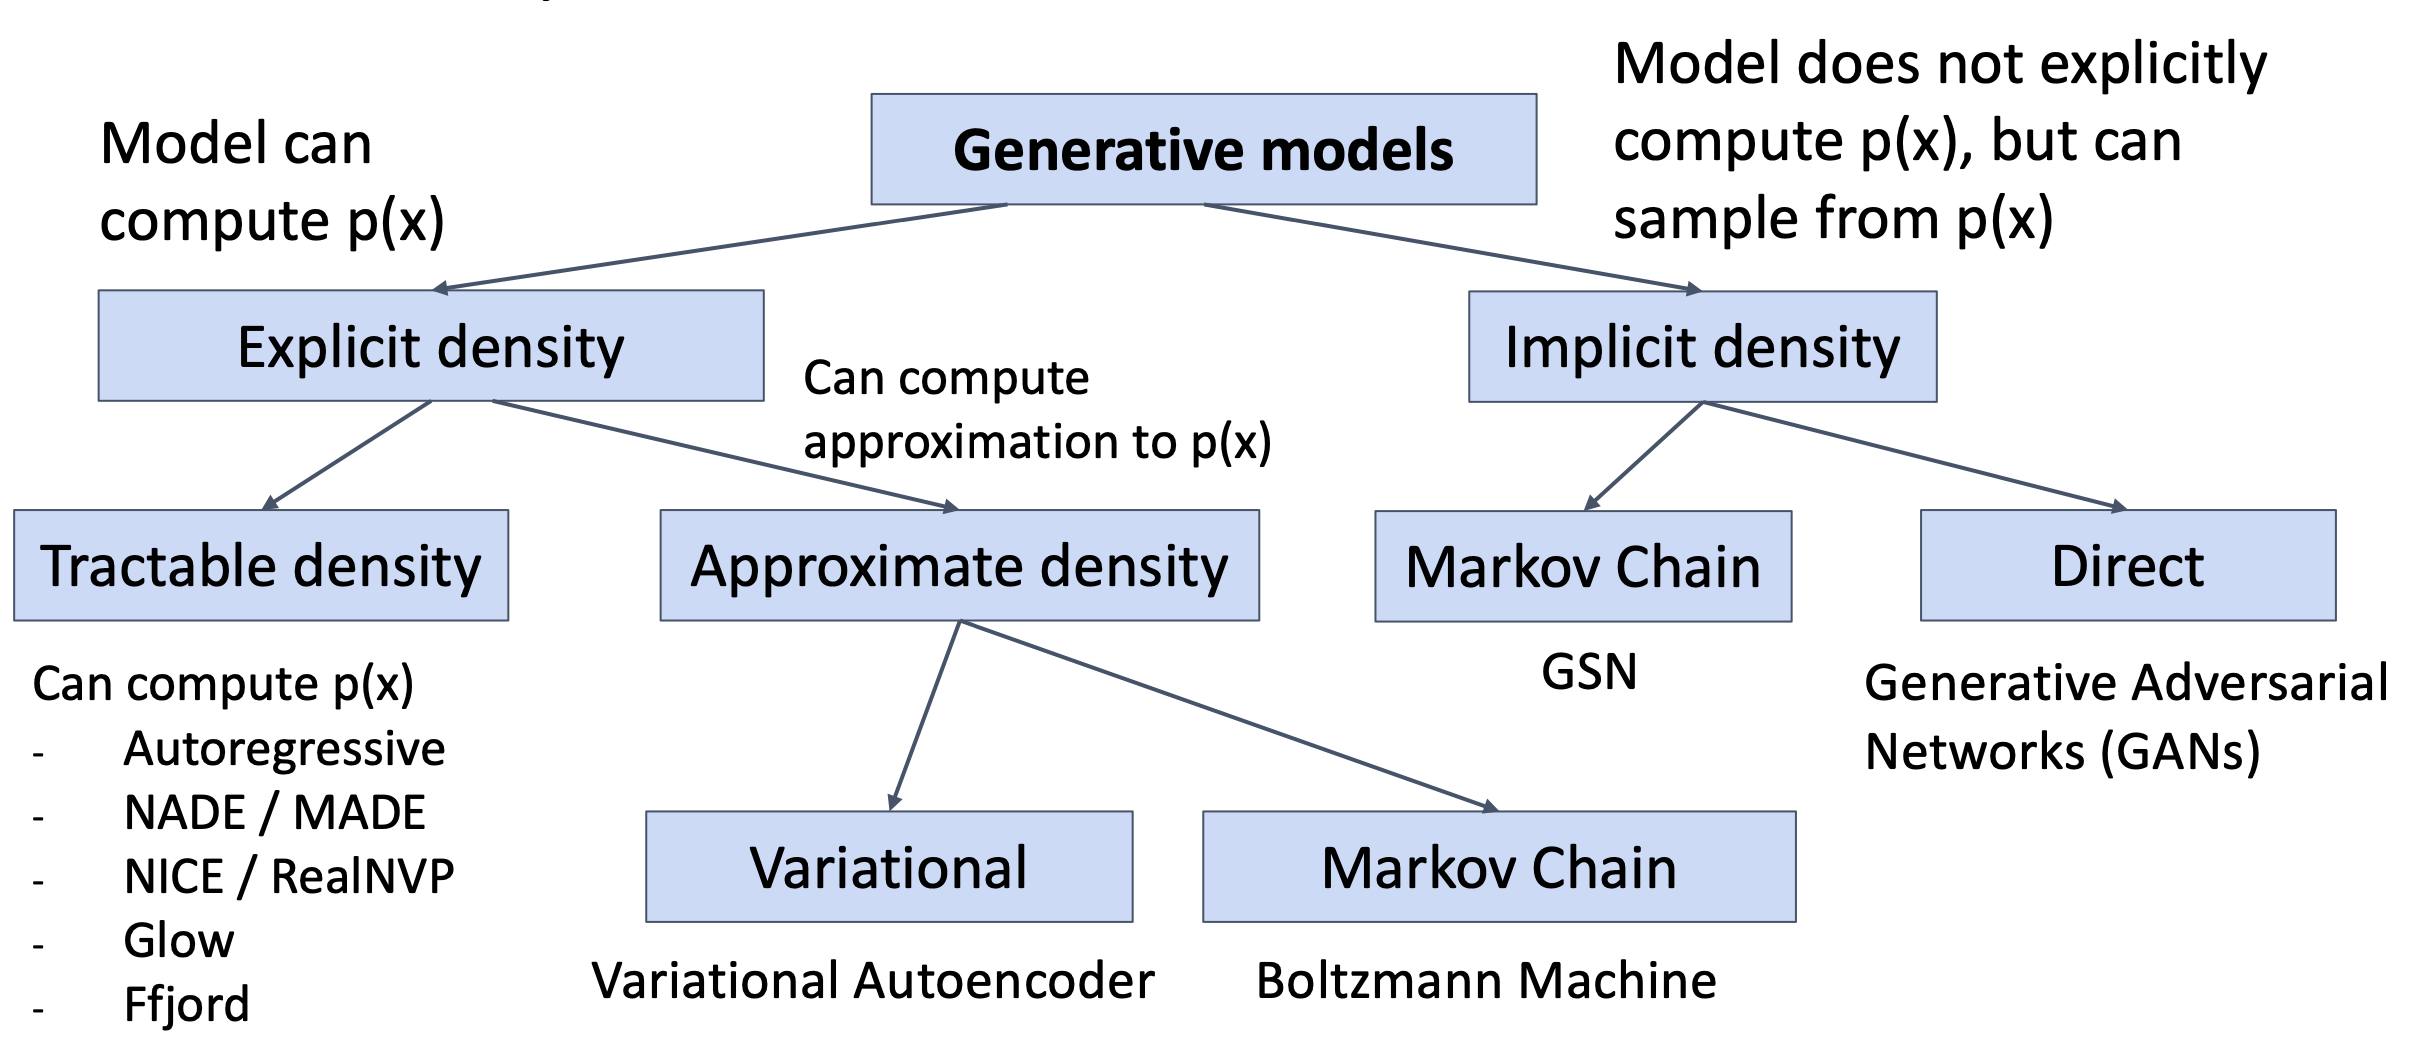
\includegraphics[width=.75\textwidth]{autoencoders/taxonomy-generative.png}
    \caption{Taxonomy of generative models}
\end{figure}
In this chapter, we will study an explicit and tractable density model family, the autoregressive models. In the next chapters, we will introduce Variational Autoencoders and Generative Adversarial Networks.

\subsection{Autoregressive Models}
\subsubsection{Explicit density estimation}
Our goal is to write an explicit function for the likelihood $\P(x)$, that is to find a parametric function $f_\theta$ such that for a certain learned value of $\theta^*$,
\begin{equation*}
    \forall x,\quad \P(x) = f_{\theta^*}(x)
\end{equation*}
Given a label-less dataset $(x^{(1)}, \dots, x^{(N)})$, we can train the model by solving the equation:
\begin{equation*}
    \begin{aligned}
        \theta^* &:= \argmax_\theta \prod_{i=1}^N \P(x^{(i)})\\
        &= \argmax_\theta \sum_{i=1}^N \log\P(x^{(i)})\\
        &= \argmax_\theta \sum_{i=1}^N \log f_\theta(x^{(i)})
    \end{aligned}
\end{equation*}
corresponding to maximum likelihood estimation. Therefore, we can simply take:
\begin{equation*}
    \L : \theta \longmapsto \sum_{i=1}^N \log f_\theta(x^{(i)})
\end{equation*}
as a loss function, and minimize it using gradient descent. In most practical applications, $\left(f_\theta\right)_\theta$ is a family of neural networks.

\subsubsection{Explicit density estimation using a regressive model}
The specificity of autoregressive models is to assume that each training sample $x^{(i)}$ consists of multiple subparts $(x_1^{(i)}, x_2^{(i)}, \dots, x_T^{(i)})$. For instance, in the case of images, each subpart can be a specific pixel.

We can break down the probability of observing a specific input by using the probability chain rule:
\begin{equation*}
    \begin{aligned}
        \P(x) &= \P(x_1, x_2, \dots, x_T)\\
        &= \P(x_1) \cdot \P(x_2|x_1) \cdot \P(x_3|x_1, x_2)\cdot \dots\\
        &= \prod_{t=1}^T \P(x_t|x_1, \dots, x_{t-1})
    \end{aligned}
\end{equation*}
This type of dependency is extremely similar to the problem solved by recurrent neural network: we want each prediction $\P(x_t|x_1, \dots, x_{t-1})$ to be conditioned on the previous time steps $x_1, \dots, x_{t-1}$. Therefore, we can train a recurrent neural network to output the successive probabilities $\P(x_t|x_1, \dots, x_{t-1})$ in a meaningful order, which can then be multiplied to obtain $\P(x)$.

\subsubsection{PixelRNN}
This is the idea of a PixelRNN: a generative model with an explicit and tractable density function, that predicts pixel values one at a time.

For each pixel, we compute a hidden state of the RNN, that depends on the hidden states and RGB values of pixels left and above:
\begin{equation*}
    h_{x,y} = f_\theta(h_{x-1,y}, h_{x, y-1})
\end{equation*}
That way, each pixel depends implicitly on all pixels left and above.
At each pixel, we can then predict the red, green, and blue values, by computing a probability distribution over $\iset{0}{255}$.
\begin{figure}[H]
    \centering
    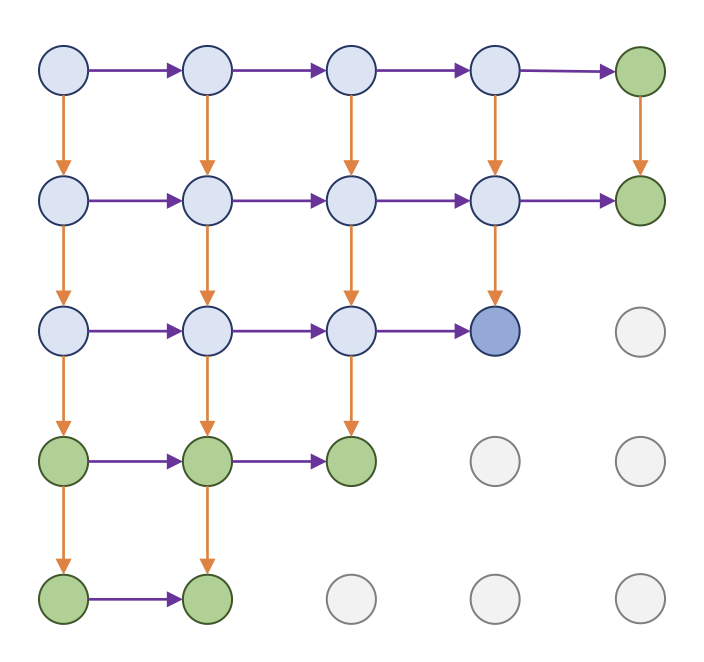
\includegraphics[width=.4\textwidth]{autoencoders/pixelrnn.png}
    \caption{Dependency of pixels in PixelRNN.}
\end{figure}

The major issue of this generative approach is that is it very slow both during training and testing.

\subsubsection{PixelCNN}
To overcome the performance issues of PixelRNN, another architecture called PixelCNN has been introduced: it still generates pixels from the top-left corner, but the dependency on each pixel is now modeled using a masked convolution over previously computed regions.
\begin{figure}[H]
    \centering
    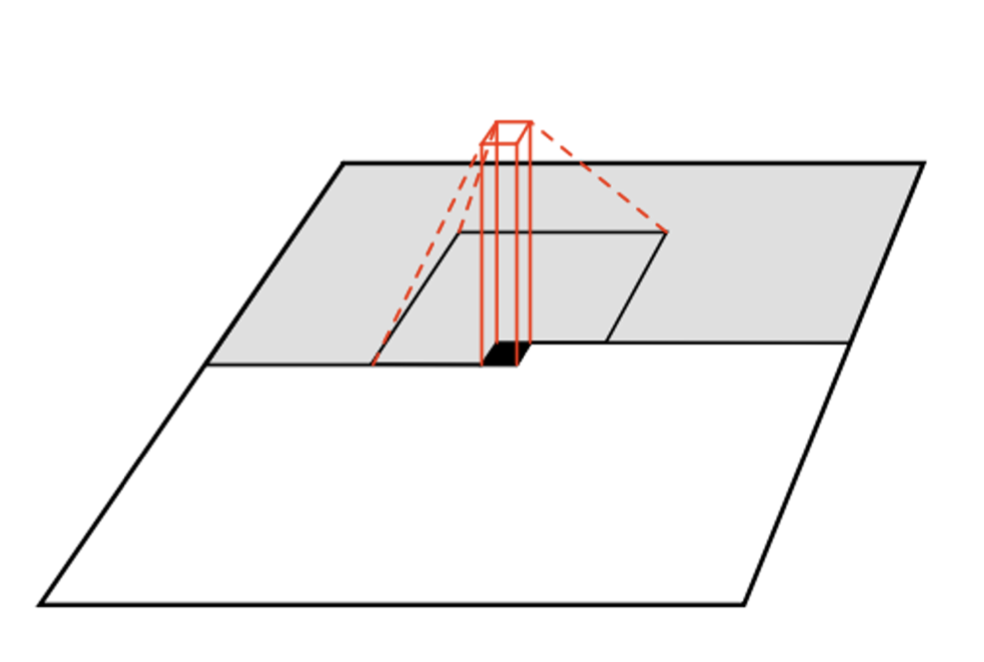
\includegraphics[width=.5\textwidth]{autoencoders/pixelcnn.png}
    \caption{Dependency of pixels in PixelCNN.}
\end{figure}
This approach allows for parallel computations of dependencies over previous pixels, making it much faster to train. It remains quite slow, because the generation must still proceed sequentially.

Generated result show that the model learned the high-level structure of the input images, by providing features such as edges and flat color shapes, but the images do not represent anything real when looked closely.\begin{figure}[H]
    \centering
    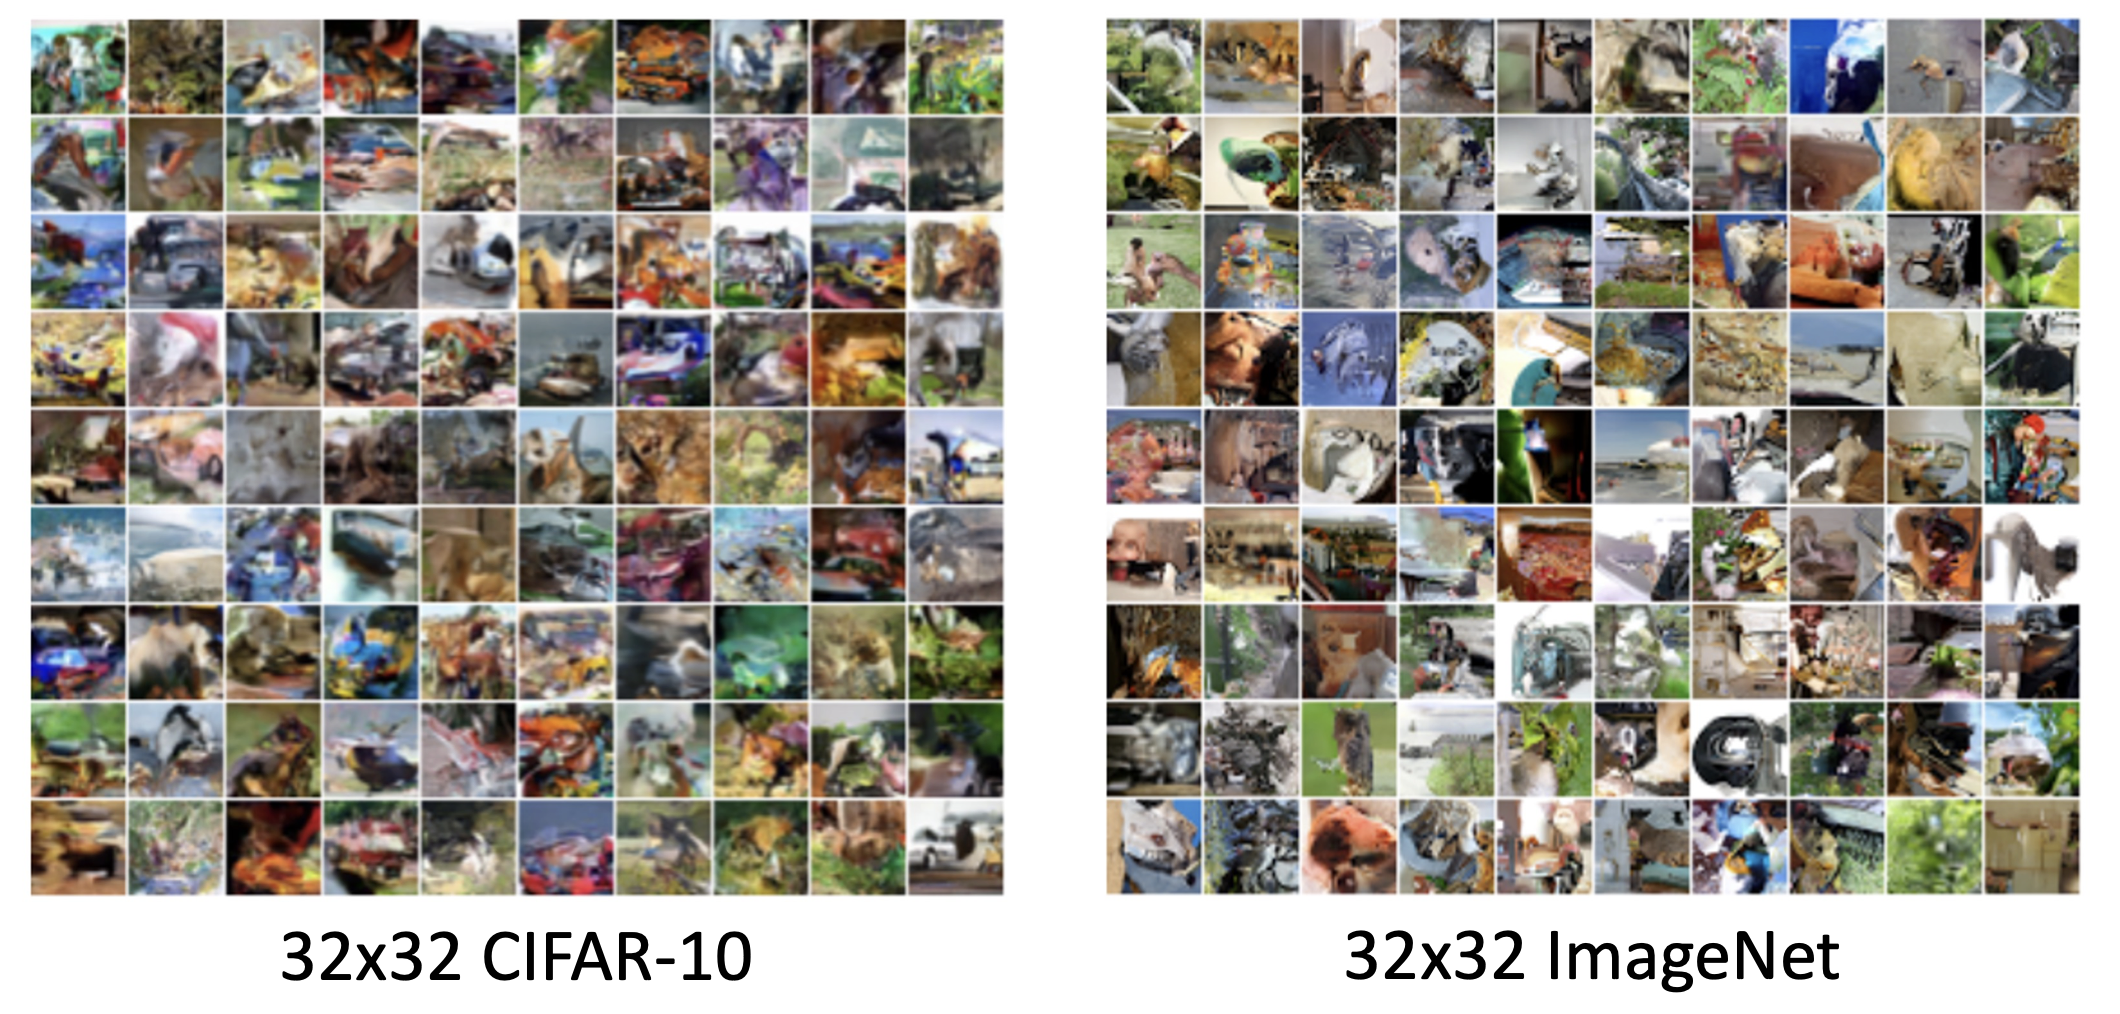
\includegraphics[width=.8\textwidth]{autoencoders/pixelcnn-results.png} 
    \caption{Results of PixelCNN.}
\end{figure}

\subsubsection{Beyond autoregressive models}
Autoregressive models have the benefit of explicitly computing the likelihood $\P(x)$, making them very easy to evaluate. Nevertheless, they require a sequential generation, making the sampling process slow.

The performance of PixelCNN can be improved with tricks in practice, such as the use of multiscale generation, gated convolutional layers or shortcut connections.

\newpage
\section{Autoencoders}
An \emph{autoencoder} is a type of neural network used to solve unsupervised learning problems. The main idea of an autoencoder is to learn an efficient representation of the input data, usually of the form of a hidden layer of size smaller than the input size. It can be useful in dimensionality reduction, but the mostly used variant is the \emph{variational autoencoder}, a certain type of generative model.

\subsection{Regular Autoencoders}
\subsubsection{Principle}
Autoencoders are designed to learn feature vectors from raw data, without any labels. Features should extract useful information, that we can use for other tasks. The main challenge is to learn this feature transform from raw data, without any idea of the form that this feature vector should take. Therefore, the idea of autoencoders is to ask the model to use these features to estimate the raw data; this way, the model will keep the features that will help it reconstruct the data, which can be intuitively considered as the \say{best} features.

An autoencoder consists of two parts: an encoder, taking into input the raw data $x$ and outputing the feature vector $z$; and a decoder, taking the feature vector $z$ as input and outputing the reconstructing input data $\hat{x}$. Both the encoder and the decoder are updated during training; the name \emph{autoencoder} shows that the model chooses its own code.
\begin{figure}[H]
    \centering
    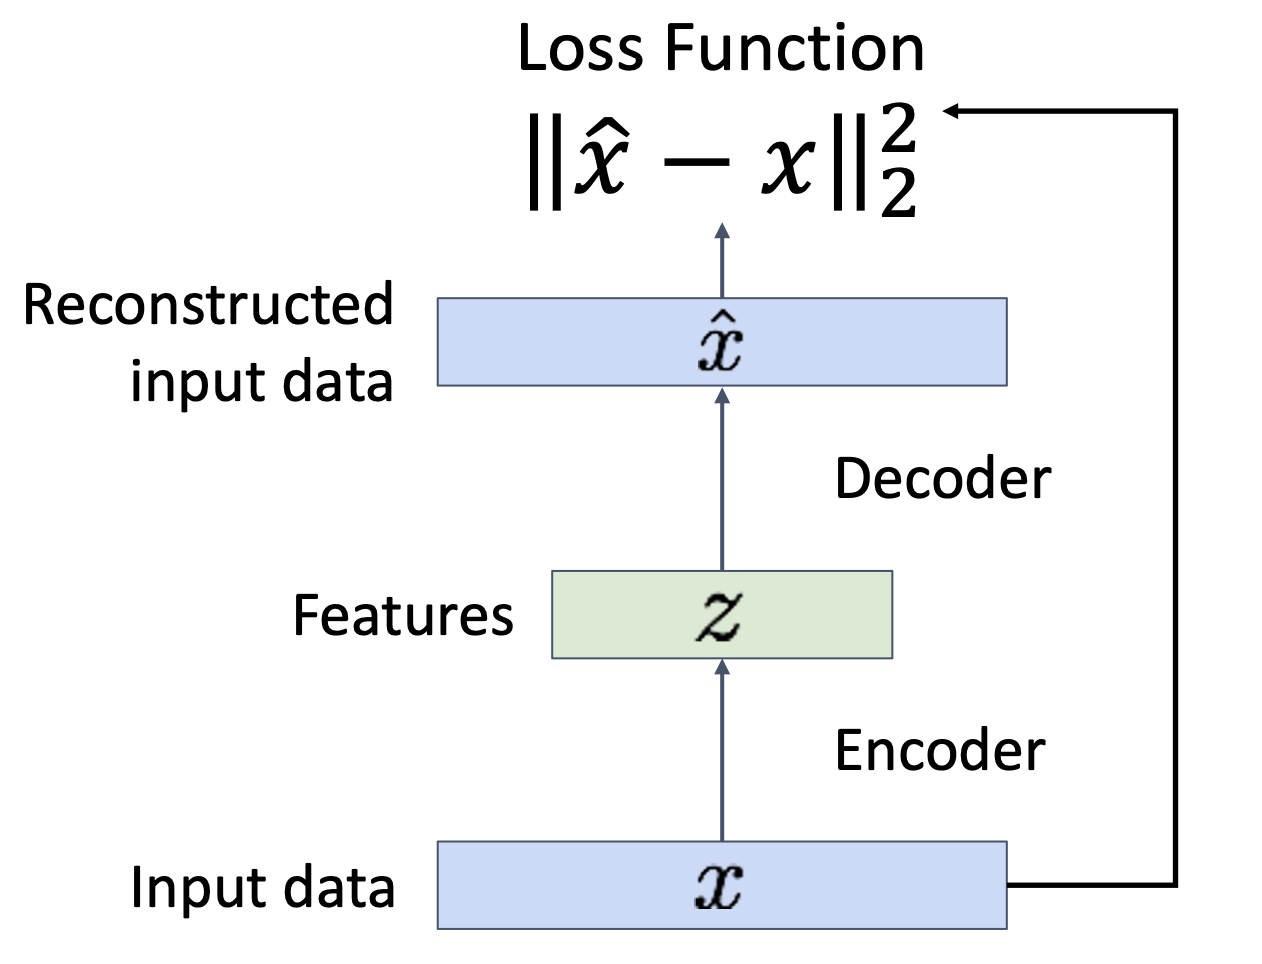
\includegraphics[width=.6\textwidth]{autoencoders/encoder-decoder.png}
    \caption{The encoder-decoder architecture of an autoencoder.}
\end{figure}
Since the goal of the decoder is to reconstruct the input data as well as possible, our loss function will be the difference between the input and the output data:
\begin{equation*}
    \L(x) = \norm{\hat{x}-x}_2^2 = \norm{f_\theta(x)-x}_2^2
\end{equation*}

In general, learning the identity function is not especially usefull and can be easily learned by a simple neural network. Therefore, features need to have a low dimension compared to the data, and act as a bottleneck. If the model approximates the identity function well, it means that the latent code (the feature vector) is an efficient way to represent the input data.

\subsubsection{Applications}
Once trained, the encoder part can be extracted and added upstream of another supervised model to solve other problems: for instance, we might add a classifier downstream and fine-tune the encoder and the classifier together.
\begin{figure}[H]
    \centering
    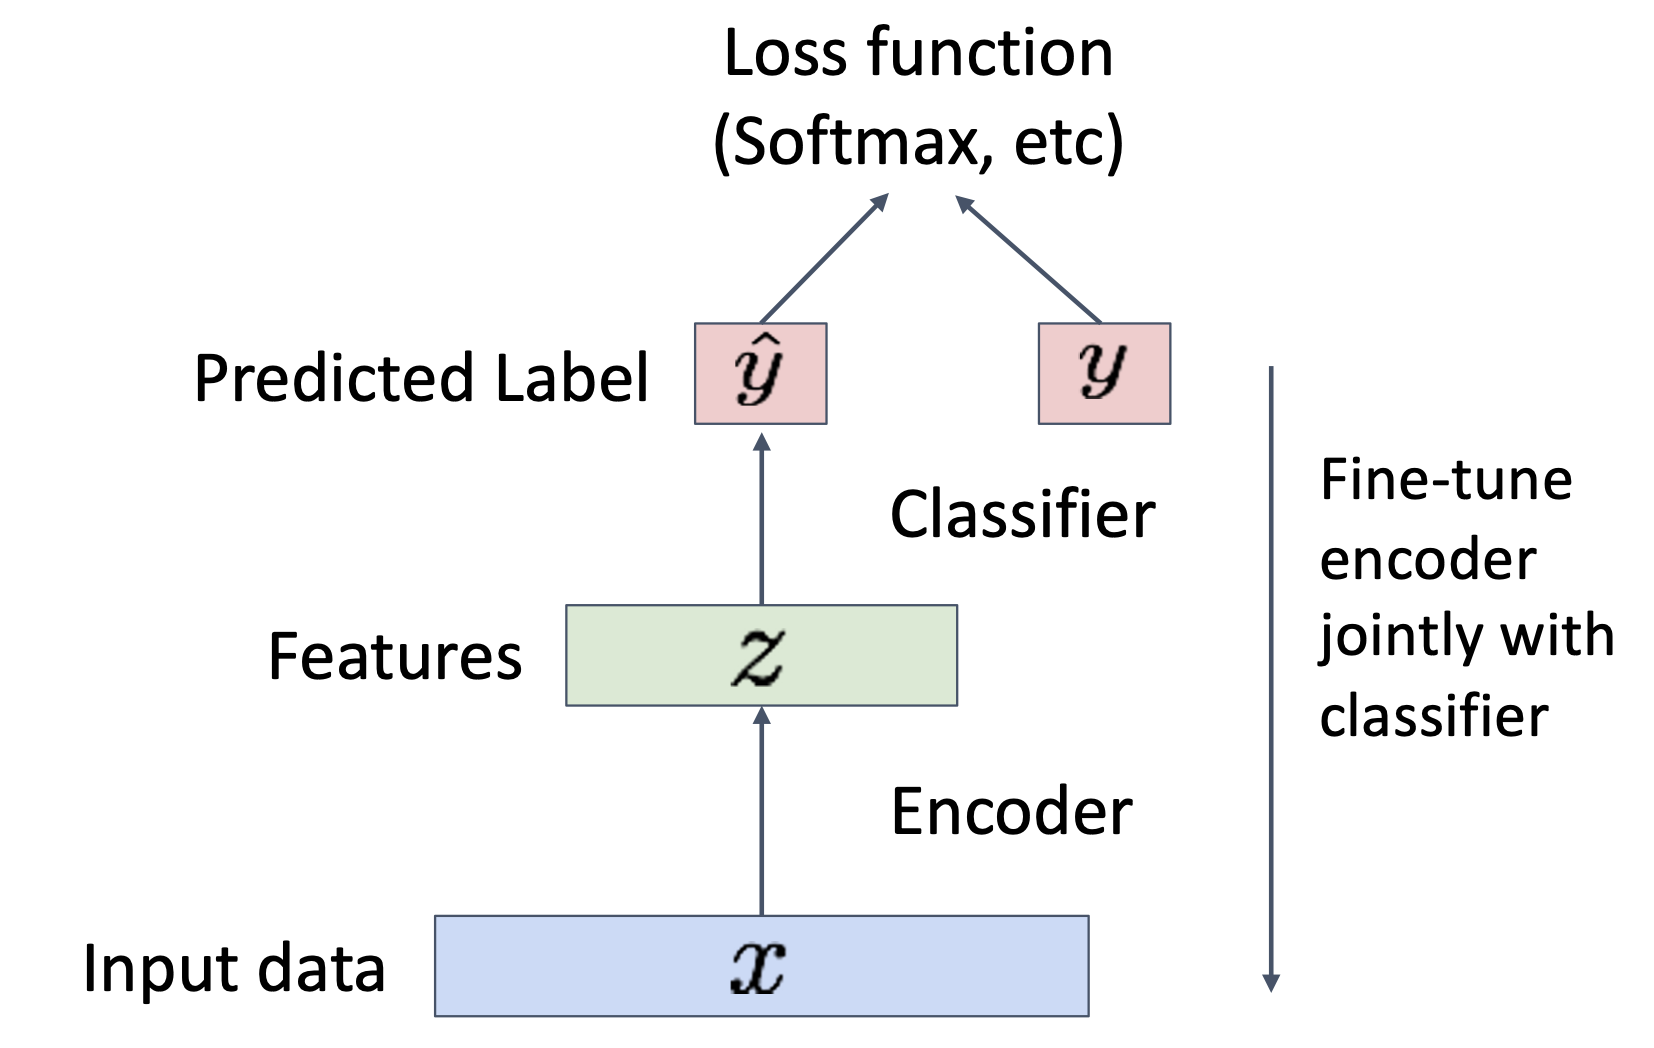
\includegraphics[width=.6\textwidth]{autoencoders/encoder-classifier.png}
    \caption{Use of the trained encoder for a downstream classification task.}
\end{figure}
One could think that we could directly train the encoder from scratch along with the classifier. In practice, training an encoder inside an autoencoder produces better results: since the autoencoder does not need labeled data, it is very simple to train on a huge amount of unlabeled inputs, producing a more robust and performant encoder.

\subsection{Variational Autoencoders}
\subsubsection{Probabilistic modelling}
We would like to adapt the autoencoder formalism to generate new inputs. Regular autoencoders are not probabilistic, and can only be used to generate the latent features $z$ of an input $x$. Instead, \emph{Variational Autoencoders} (VAEs) will be used to learn a probability distribution, from which we can sample new data.

Formally, we assume that our training data $(x^{(i)})_{i\in\iset{1}{N}}$ is generated from a latent representation $z$, to which we do not have access to. After training, the variational autoencoder will proceed in two steps to output a probability distribution over new inputs. First, it will sample a certain feature vector $z$ from some learned prior distribution $\P_{\theta^*}(z)$. Then, it will use this generated latent representation to output the conditional probability distribution $\P_{\theta^*}(x|z)$.
\begin{figure}[H]
    \centering
    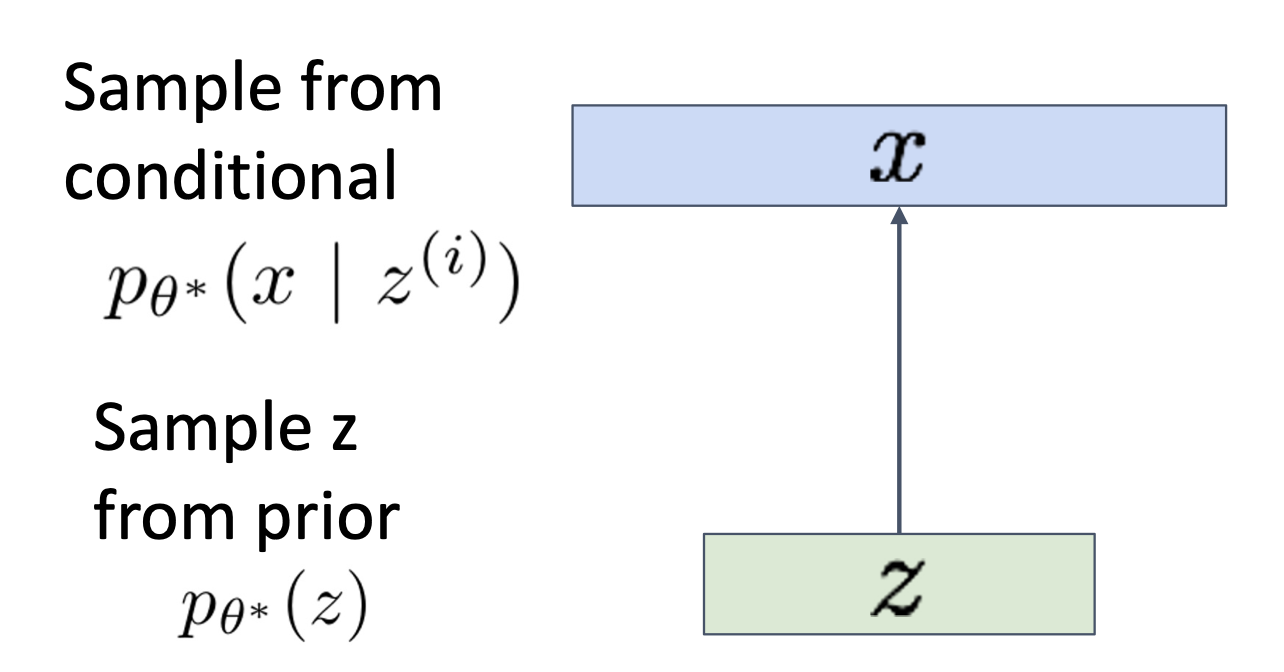
\includegraphics[width=.5\textwidth]{autoencoders/variational-principle.png}
\end{figure}

The prior distribution $\P_{\theta^*}(z)$ can be assumed to be very simple, such as a Gaussian distribution over $\R^d$. The conditional distribution $\P_{\theta^*}(x|z)$ will be represented with a neural network, similar to the decoder of an autoencoder. To do so, we will output the parameters of a parametrized output distribution. For instance, we can output a vector $\mu_{x|z}$ and a diagonal matrix $\Sigma_{x|z}$, and say that the associated distribution is the Gaussian distribution over $\R^d$ of mean $\mu_{x|z}$ and covariance matrix $\Sigma_{x|z}$.
\begin{figure}[H]
    \centering
    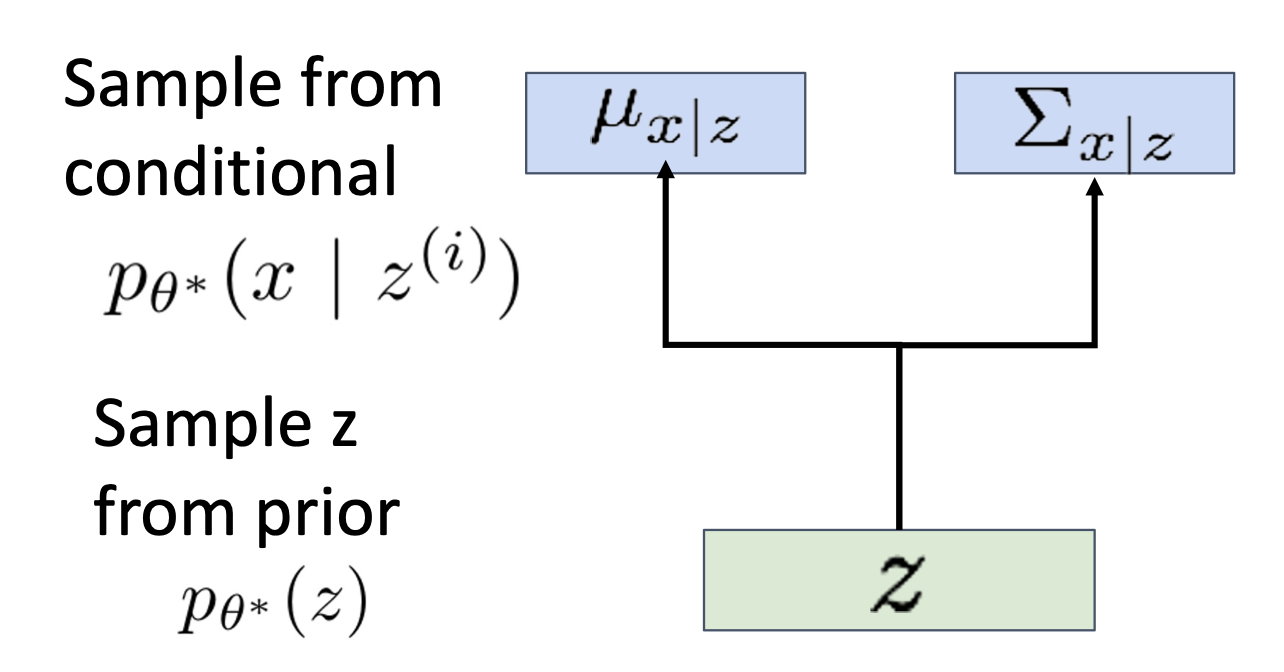
\includegraphics[width=.5\textwidth]{autoencoders/gaussian-parameters.png}
\end{figure}

\subsubsection{Variational lower bound}
To train the variational autoencoder, we maximize the likelihood of the data. Given the latent vectors $(z^{(i)})_{i\in\iset{1}{N}}$, we could train the conditional generative model part directly, but we do not have access to $z$. Therefore, we will jointly train two parts, just like for regular autoencoders: an encoder that inputs data $x$, and outputs a distribution over the latent codes $z$, and a decoder that inputs a latent code $z$ and outputs a distribution over the data $x$.

\begin{figure}[H]
    \centering
    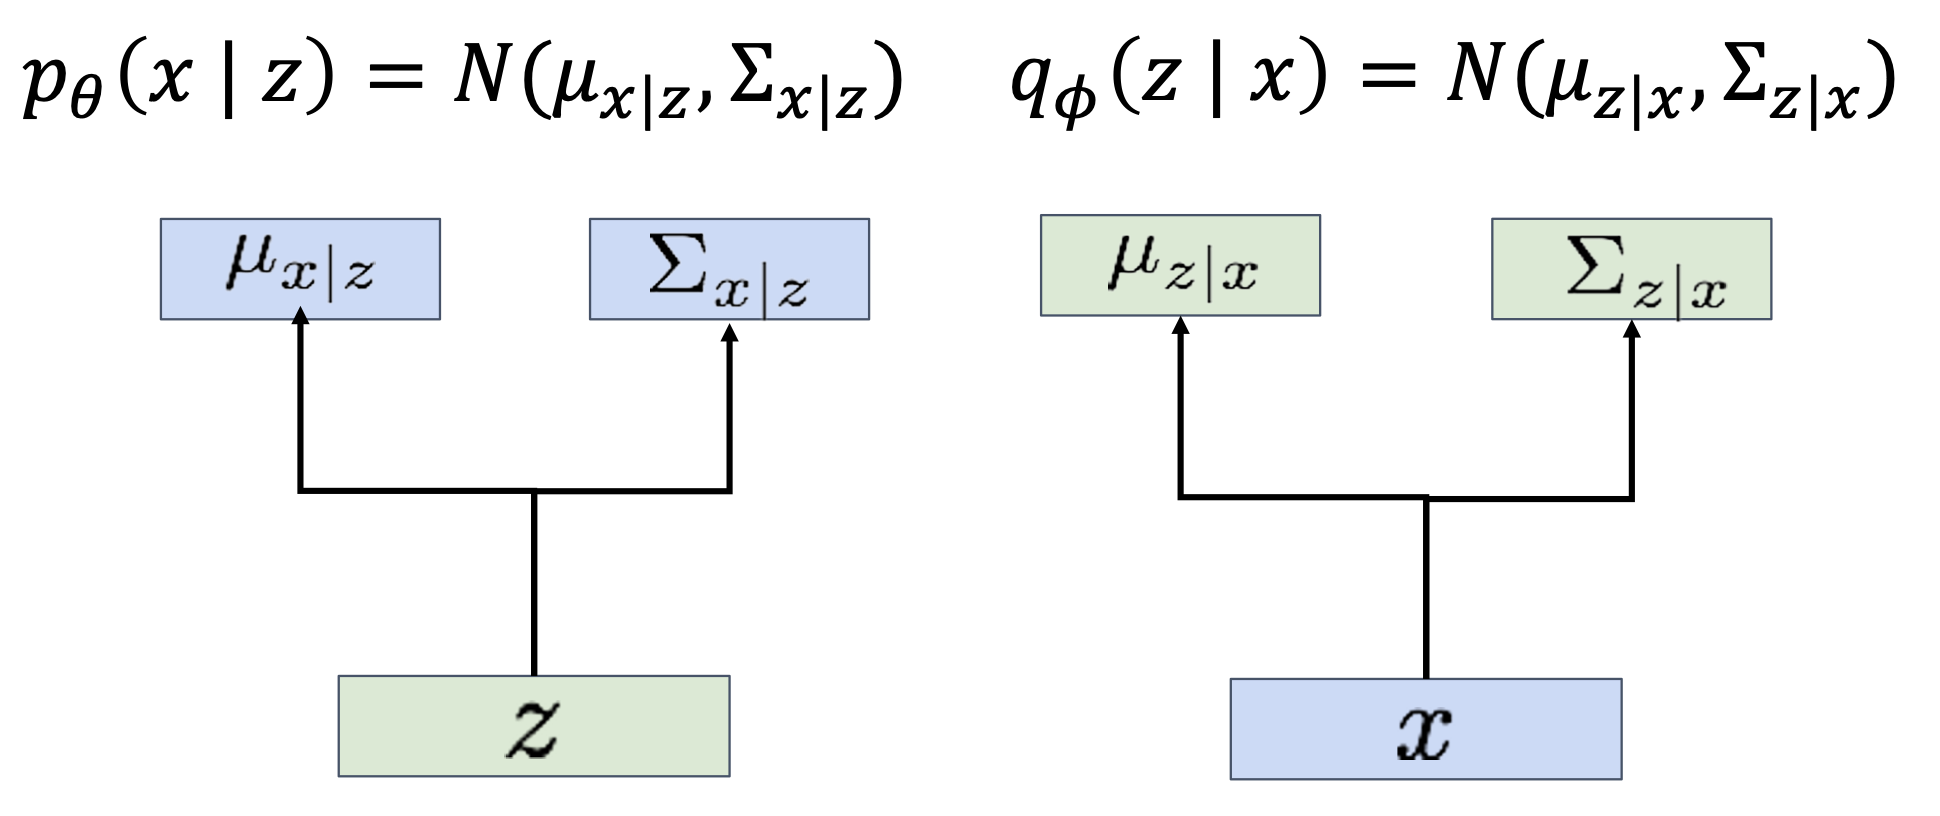
\includegraphics[width=.6\textwidth]{autoencoders/variational-encoder-decoder.png}
\end{figure}

Note that according to Bayes' rule:
\begin{equation*}
    \P_\theta(x) = \frac{\P_\theta(x|z)\cdot \P_\theta(z)}{\P_\theta(z|x)}
\end{equation*}
The probability $p_\theta(x|z)$ is computed by the network taking into input $z$ and outputing the Gaussian parameters. We assumed $z$ to be sampled from a Gaussian distribution, we therefore know $\P_\theta(z)$. Finally, $\P_\theta(z|x)$ is estimated by the encoder.

\begin{property}[Variational lower bound]
    The following inequality holds for any distributions $p_\theta$ and $q_\varphi$:
    \begin{equation}
        \label{eq:variational-lower-bound}
        \log p_\theta(x) \geq \E_{z\sim q_\varphi(z|x)}\left[\log p_\theta(x|z)\right] - \KL\left(q_\varphi(z|x)\parallel p_\theta(x)\right)
    \end{equation}
    where $\KL$ denotes the Kullback-Leibler divergence.
\end{property}
\begin{proof}
    We decompose $p_\theta(x)$:
    \begin{align*}
        \log p_\theta(x) &= \log\frac{p_\theta(x|z)\cdot p(z)}{p_\theta(z|x)} && \text{(Bayes' rule)} \\
        &= \log\frac{p_\theta(x|z)\cdot p(z)\cdot q_\varphi(z|x)}{p_\theta(z|x)\cdot q_\varphi(z|x)} \\
        &= \log p_\theta(x|z) - \log\frac{q_\varphi(z|x)}{p(z)} + \log\frac{q_\varphi(z|x)}{p_\theta(z|x)} \\
        &= \E_{z\sim q_\varphi(z|x)}\left[\log p_\theta(x|z)\right] - \E_{z\sim q_\varphi(z|x)}\left[\log\frac{q_\varphi(z|x)}{p(z)}\right] + \E_{z\sim q_\varphi(z|x)}\left[\log\frac{q_\varphi(z|x)}{p_\theta(z|x)}\right] \\
        &= \E_{z\sim q_\varphi(z|x)}\left[\log p_\theta(x|z)\right] - \KL\left(q_\varphi(z|x)\parallel p(z)\right) + \KL\left(q_\varphi(z|x)\parallel p_\theta(z|x)\right)
    \end{align*}
    Since the Kullback-Leibler divergence is always positive, we can ommit the rightmost term and obtain:
    \begin{equation*}
        \log p_\theta(x) \geq \E_{z\sim q_\varphi(z|x)}\left[\log p_\theta(x|z)\right] - \KL\left(q_\varphi(z|x)\parallel p_\theta(x)\right)
    \end{equation*}
\end{proof}

We will train the encoder and decoder of the variational autoencoder by maximizing the \emph{Evidence Lower Bound} \autoref{eq:variational-lower-bound}.

% TODO: move this subsubsection and the next one before variational lower bound?
\subsubsection{Example: Fully-connected Variational Autoencoder}
To give a concrete example, let's imagine that we want to train a variational autoencoder on the MNIST dataset to generate new images. The input data $x$ is a flatted $28\times28$ image, therefore $x\in\R^{784}$; we choose the latent space to be $z\in\R^{20}$. We choose both the encoder and the decoder network to be fully-connected networks as described in \autoref{fig:fully-connected-vae}.
\begin{figure}[H]
    \centering
    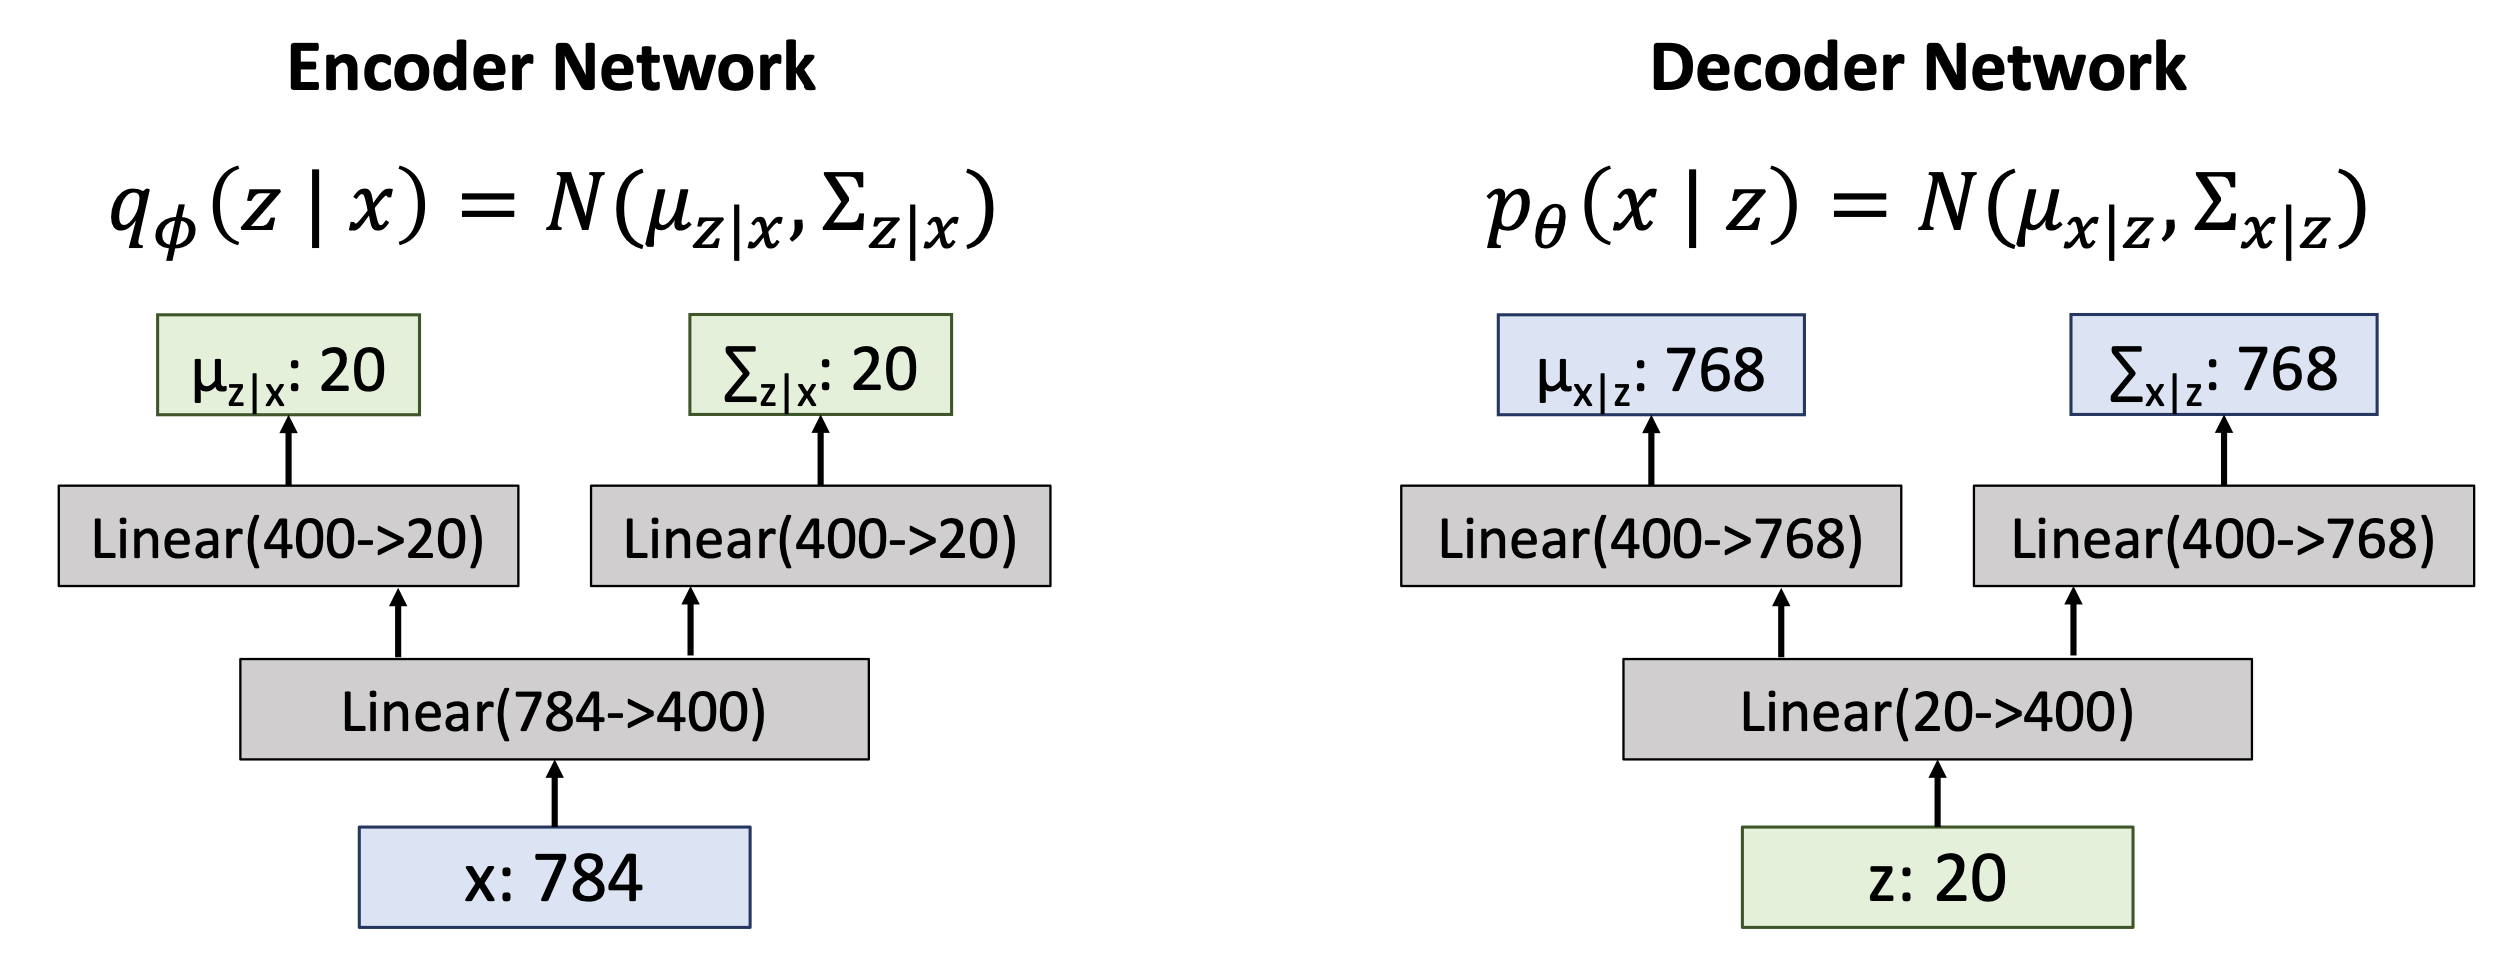
\includegraphics[width=.8\textwidth]{autoencoders/fully-connected-vae.png}
    \caption{A fully-connected variational autoencoder.}
    \label{fig:fully-connected-vae}
\end{figure}

\subsubsection{Forward pass during training}
The forward pass of a variational autoencoder is very similar to the one of a regular autoencoder, except that both the encoder and the decoder output Gaussian parameters. Therefore, we can compute the output data distribution in three simple steps:
\begin{itemize}
    \item First, we feed the input data $x$ to the encoder, which outputs the mean $\mu_{z|x}$ and the diagonal covariance matrix $\Sigma_{z|x}$ of the latent distribution.
    \item Then, we sample a latent vector $z$ from this distribution $\Nc(\mu_{z|x}, \Sigma_{z|x})$.
    \item Finally, we feed this latent vector to the decoder, which outputs the mean $\mu_{x|z}$ and the diagonal covariance matrix $\Sigma_{x|z}$ of the output distribution.
\end{itemize}
We can then sample a new data point $\hat{x}$ from this distribution $\Nc(\mu_{x|z}, \Sigma_{x|z})$.
\begin{figure}[H]
    \centering
    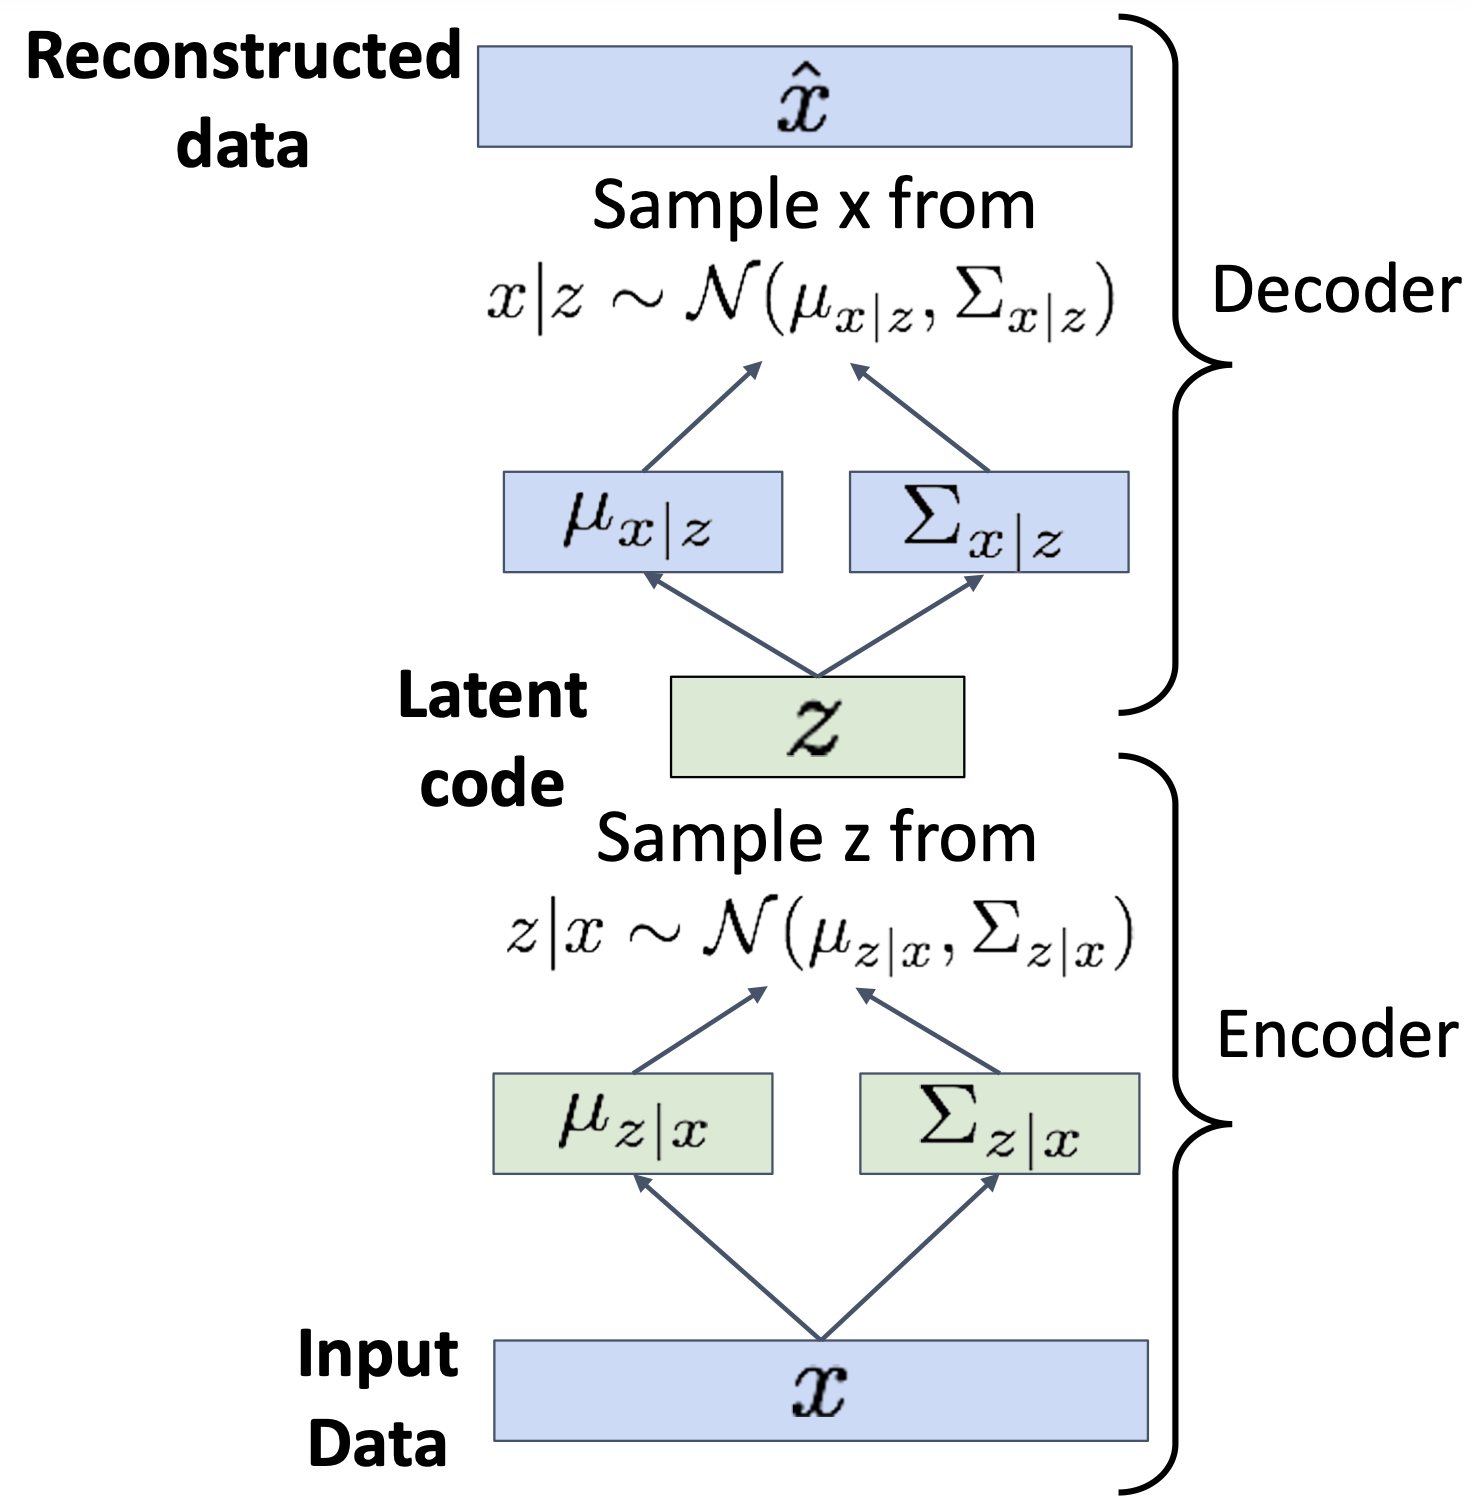
\includegraphics[width=.55\textwidth]{autoencoders/vae-training.png}
    \caption{The successive steps of a forward pass of a VAE during training.}
\end{figure}


\subsubsection{Loss computation during training}
Recall that to train the model, we will maximize the lower bound of the probability:
\begin{equation*}
    \L(x) = \E_{z\sim q_\varphi(z|x)}\left[\log p_\theta(x|z)\right] - \KL\left(q_\varphi(z|x)\parallel p_\theta(x)\right)
\end{equation*}
The two terms of this loss function can be computed during the forward pass of the model. Given the distribution over $z$, the Kullback-Leibler divergence term can be computed analytically, since we assumed a simple form for the prior distribution -- a unit Gaussian. The first term -- the expectation -- can be computed by sampling $z$ and computing the $\log$-likelihood of the output data given this latent vector.

More specifically, the KL term can be computed as:
\begin{equation*}
    \begin{aligned}
        -\KL\left(q_\varphi(z|x)\parallel p(z)\right) &= \int_z q_\varphi(z|x)\cdot\log\frac{p(z)}{q_\varphi(z|x)}\dd z\\
        &= \int_z N(z; \mu_{z|x}, \Sigma_{z|x})\cdot\log\frac{N(z; 0, I_d)}{N(z; \mu_{z|x}, \Sigma_{z|x})}\dd z\\
        &= \frac{1}{2}\sum_{k=1}^d \left(1 + \log\left(\Sigma_{z|x}\right)^2_j - \left(\mu_{z|x}\right)^2_j - \left(\Sigma_{z|x}\right)^2_j\right)
    \end{aligned}
\end{equation*}
where $N$ is the probability density of the Gaussian distribution\footnote{That is $N(z; \mu, \Sigma) = \frac{1}{(2\pi)^{d/2}|\Sigma|^{1/2}}\cdot\exp\left[-\frac{1}{2}(x-\mu)^\tp\Sigma^{-1}(x-\mu)\right]$}.

\newpage
\section{Generative Adversarial Networks}
\subsection{Introduction}
So far, we have seen two generative models, autoregressive models and variational autoencoders. Both of these approaches try to model $\P(x)$; autoregressive models directly maximize the likelihood of the data:
\begin{equation*}
    p_\theta(x) = \prod_{i=1}^N p_\theta(x_i|x_1, \dots, x_{i-1})
\end{equation*}
while variational autoencoders maximize the evidence lower bound:
\begin{equation*}
    \log p_\theta(x) \geq \E_{z\sim q_\varphi(z|x)}\left[\log p_\theta(x|z)\right] - \KL\left(q_\varphi(z|x)\parallel p(z)\right)
\end{equation*}
Both of these models have their limitations; autoregressive models are slow to sample from, and variational autoencoders can have blurry samples. Generative adversarial networks (GANs) are a third approach to generative modeling that can generate high-quality samples quickly, by focusing on the problem of generating samples from a distribution instead of trying to explicitly model the distribution.

\subsection{Generator and Discriminator}
Assume that we have acces to some data samples $x_i$ drawn from a certain distribution $p_{\text{data}}$. Our goal is to draw new samples from $p_{\text{data}}$, without trying to access its values. Similarly to variational autoencoders, we assume that each sample is associated to a latent variable $z$ with a simple prior distribution $p(z)$. The idea is to learn a \emph{Generator Network} $G(z)$ that takes a latent variable $z$ as input and outputs a sample $x = G(z)$. $G$ implicitely defines a probability distribution $p_G$ over the samples $x$; we want to learn $G$ such that $p_G$ is as close as possible to $p_{\text{data}}$.

In parallel, we will train a \emph{Discriminator Network} $D$ to perform a classification task: given a sample $x$, $D(x)$ should output the probability that $x$ is a sample from $p_{\text{data}}$ rather than $p_G$. The training of $D$ is supervised: it is trained on both real samples $x_i$ and fake samples $G(z)$, of which we know the labels $0$ and $1$ respectively.
\begin{figure}[H]
    \centering
    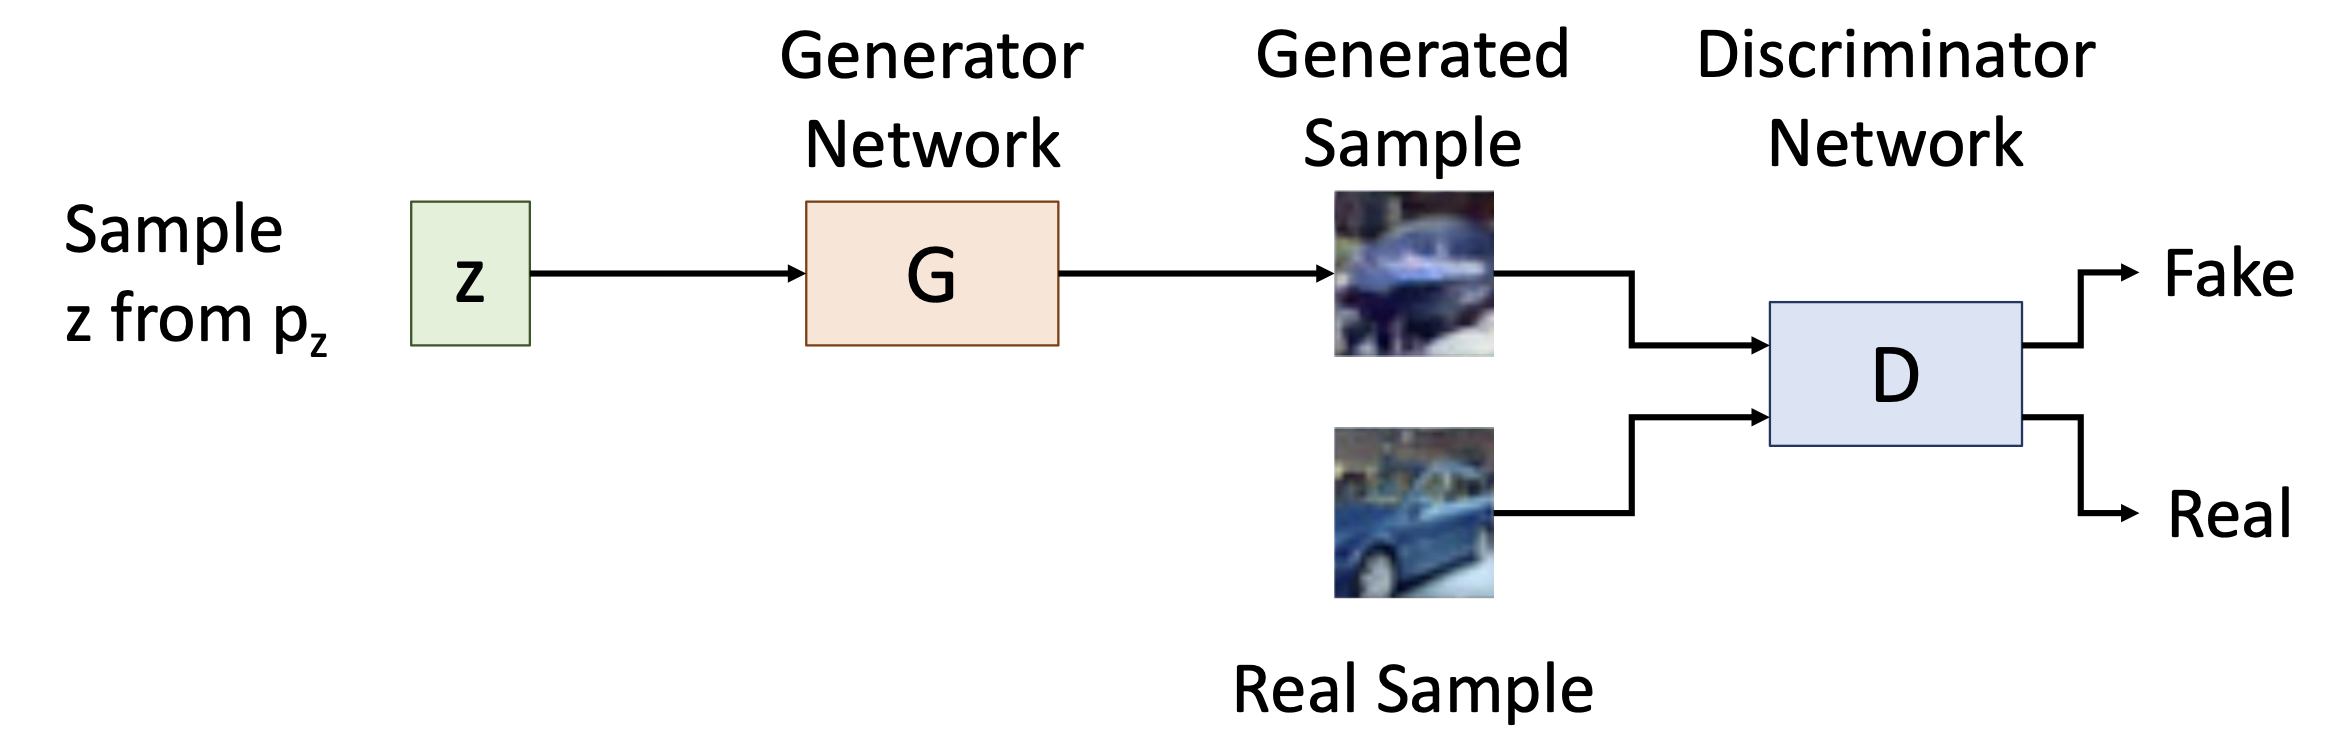
\includegraphics[width=.9\textwidth]{gans/generator-discriminator.png}
\end{figure}
We train the Generator $G$ and the Discriminator $D$ in an \emph{adversarial} manner: $G$ tries to fool $D$ by generating samples that are indistinguishable from real samples, while $D$ tries to distinguish between real and fake samples.

\subsection{Training objective}
We will jointly train the Generator $G$ and the Discriminator $D$ with a \emph{minimax game}. A first objective to optimize for is the following:
\begin{equation}
    \min_G\max_D \left(
        \E_{x\sim p_{\text{data}}}\left[\log D(x)\right] + \E_{z\sim p(z)}\left[\log\left(1-D\left(G(z)\right)\right)\right]
    \right)
\end{equation}
The Discriminator wants $D(x)=1$ for real data and $D(x)=0$ for fake data. Therefore, the first inner quantity $\E_{x\sim p_{\text{data}}}\left[\log D(x)\right]$ is the $\log$-likelihood of a real sample being classified as real, while the second inner quantity $\E_{z\sim p(z)}\left[\log\left(1-D\left(G(z)\right)\right)\right]$ is the $\log$-likelihood of a fake sample being classified as fake. The objective of the Discriminator is to maximize both these quantities, while the Generator tries to minimize them.

Let $V(G, D) = \E_{x\sim p_{\text{data}}}\left[\log D(x)\right] + \E_{z\sim p(z)}\left[\log\left(1-D\left(G(z)\right)\right)\right]$. The training loop will consist in alternating between the optimization of $D$ and $G$; for $t\in\iset{0}{T}$:
\begin{enumerate}
    \item Update $D$: \begin{equation*}D\longleftarrow D+\alpha_D\frac{\partial V}{\partial D}\end{equation*}
    \item Update $G$: \begin{equation*}G\longleftarrow G-\alpha_G\frac{\partial V}{\partial G}\end{equation*}
\end{enumerate}
Note that we are not minimizing any overall loss; the generator and the discriminator have their own loss, which depend on each other and is usually not monotonically decreasing.

In practice, at the start of training, the generator performs quite poorly while the dicriminator can easily tell apart real and fake data, making $D(G(z))$ very close to $0$. This usually leads to a vanishing gradient for $G$. To avoid this, instead of training $G$ to minimize $\log\left(1-D(G(z))\right)$, we train it to minimize $-\log D(G(z))$.

\subsection{Optimality}
We hope that jointly training $G$ and $D$ will make the generator's distribution $p_G$ converge to $p_{\text{data}}$. We will analytically derive the optimal discriminator and generator to show that this is the case.

First, note that:
\begin{align*}
    &\min_G\max_D \left(
        \E_{x\sim p_{\text{data}}}\left[\log D(x)\right] + \E_{z\sim p(z)}\left[\log\left(1-D\left(G(z)\right)\right)\right]
    \right) \\
    = &\min_G\max_D \left(
        \E_{x\sim p_{\text{data}}}\left[\log D(x)\right] + \E_{x\sim p_G}\left[\log\left(1-D(x)\right)\right]
    \right) && \text{(change of variables)} \\
    = &\min_G\max_D
        \int_X \left( p_{\text{data}}(x)\cdot\log D(x) + p_G(x)\cdot\log\left(1-D(x)\right) \right) \dd x
     && \text{(definition of $\E$)} \\
    = &\min_G
        \int_X \max_D \left[ p_{\text{data}}(x)\cdot\log D(x) + p_G(x)\cdot\log\left(1-D(x)\right) \right] \dd x
     && \text{(functions are well-behaved)} \\
\end{align*}

We can now derive the optimal discriminator $D_G^*$. Note that the quantity inside the $\max_D$,
\begin{equation*}
    p_{\text{data}}(x)\cdot\log D(x) + p_G(x)\cdot\log\left(1-D(x)\right)
\end{equation*}
is of the form:
\begin{equation*}
    f(y) = a\cdot\log y + b\cdot\log(1-y)
\end{equation*}
We have that $f'(y) = \frac{a}{y} - \frac{b}{1-y} = 0$ when $y = \frac{a}{a+b}$. Therefore, the optimal discriminator is:
\begin{equation*}
    D_G^*(x) = \frac{p_{\text{data}}(x)}{p_{\text{data}}(x) + p_G(x)}
\end{equation*}

We can continue the computation to find the optimal generator $G^*$. We have:
\begin{align*}
    &\min_G\max_D \left(
        \E_{x\sim p_{\text{data}}}\left[\log D(x)\right] + \E_{z\sim p(z)}\left[\log\left(1-D\left(G(z)\right)\right)\right]
    \right) \\
    = &\min_G
        \int_X \left( p_{\text{data}}(x)\cdot\log D^*_G(x) + p_G(x)\cdot\log\left(1-D^*_G(x)\right) \right) \dd x \\
    = &\min_G
        \int_X \left( p_{\text{data}}(x)\cdot\log\left(\frac{p_{\text{data}}(x)}{p_{\text{data}}(x) + p_G(x)}\right) + p_G(x)\cdot\log\left(1-\frac{p_{\text{data}}(x)}{p_{\text{data}}(x) + p_G(x)}\right) \right) \dd x \\
    = &\min_G
        \left( \E_{x\sim p_{\text{data}}}\left[\log\frac{p_{\text{data}}(x)}{p_{\text{data}}(x) + p_G(x)}\right] + \E_{x\sim p_G}\left[\log \frac{p_{\text{data}}(x)}{p_{\text{data}}(x) + p_G(x)}\right] \right) \\
\end{align*}
To obtain a simpler expression, we multiply by a factor $2$ to make the Kullback-Leibler divergence appear:
\begin{align*}
    &\phantom{=}\min_G\max_D \left(
        \E_{x\sim p_{\text{data}}}\left[\log D(x)\right] + \E_{z\sim p(z)}\left[\log\left(1-D\left(G(z)\right)\right)\right]
    \right) \\
    &=\min_G
        \left( \E_{x\sim p_{\text{data}}}\left[\log\frac{2\cdot p_{\text{data}}(x)}{p_{\text{data}}(x) + p_G(x)}\right] + \E_{x\sim p_G}\left[\log \frac{2\cdot p_{\text{data}}(x)}{p_{\text{data}}(x) + p_G(x)}\right]\right) - \log4 \\
    &= \min_G
        \left(\KL\left(
            p_{\text{data}}\parallel\frac{p_{\text{data}}+p_G}{2}
        \right) + \KL\left(
            p_G\parallel\frac{p_{\text{data}}+p_G}{2}
        \right)\right) - \log4 \\
    &= 2\times\min_G \JSD(p_{\text{data}}\parallel p_G) - \log4 \\
\end{align*}
Hence, since the Jensen-Shannon divergence is always non-negative, and zero if and only if the two distributions are equal, $p_{\text{data}} = p_G$. Therefore, the optimal generator for the optimal $D$ is the data distribution itself.

Even though we have no guarantee that we can actually represent the optimal $D$ and $G$, this shows that the GAN training objective is well-posed and can converge to the optimal solution if the networks are expressive enough.

\subsection{Results}

\subsection*{Generative Adversarial Networks: Summary}

\newpage

\section{Normalizing Flows}

\end{document}